\documentclass[11pt]{article}
\usepackage[dvips]{graphicx}
\oddsidemargin 0in
\textheight 9.in
\textwidth 6.5in
\topmargin -0.50in
\parskip .29cm
\renewcommand{\baselinestretch}{1.2}
\baselineskip 1.2cm
\newenvironment{references}[0]{
\parindent -15pt}{}
%
\newcommand{\dfrac}{\displaystyle \frac}
\newcommand{\vred}{\vspace {-0.1in}}

\begin{document}

\vspace{30pt}

\title{\vspace{20pt}
{\bf \Huge The Mineos Package}\\
{\bf V 1.0}  \\
{\bf \emph{by}} \\
{\bf \emph{Guy Masters}} \\
\vspace{25pt}
{\bf User's manual} \\
\vspace{42pt}
\vspace{100pt}
\vspace{100pt}
}
\author{
Software Package and Documentation Prepared by:\\
Misha Barmine\\
University of Colorado at Boulder\\
Send comments, questions, suggestions to:
\textbf{\emph{barmin@ciei.colorado.edu}}  \\ \\
\large Funding and Support Provided By: \\
\large Computational Infrastructure for Geodynamics (CIG)\\ \normalsize}

\date {{November 26, 2006}}

\maketitle


\newpage

\renewcommand{\baselinestretch}{1.0}
\tableofcontents
\renewcommand{\baselinestretch}{1.2}

\newpage

\section{Mineos Package Overview}

The {\bf Mineos Package}, by Guy Masters, consists of four programs:
{\bf minos\_bran, eigcon, green,} and {\bf syndat}. Functionally,
the programs break into two sub-groups. The first sub-group contains
the programs that produce the normal mode eigenfunctions and eigenfrequencies,
{\bf minos\_bran} and {\bf eigcon}. Information flow into and out of these
two programs, which we call the {\it eigenfunction system},
is summarized in Figure 1. The second sub-group, referred to as the
{\it synthetic seismogram system}, comprises
the programs that read the output from {\bf eigcon} and compute Green
functions and synthetic seismograms. These programs are {\bf green}
and {\bf syndat} and information flow through these programs is
summarized in Figure 2.

The four programs are executed in sequence.
Some of the the most important files that are produced along the way 
and at the end are formatted into an extension of the CSS-3.0 relational
data base schema. Each file is an ascii flat file that can be read
with a text editor, but has the advantage of also being subsumable into
a data base system such as ORACLE, Postgress, MySql, or Antelope. 
This {\it multi-tiered access} is a design goal of the I/O system
of the {\bf Mineos} package. The potential disadvantage of using
the relational database framework is that the files in the schema
are formatted ascii files that are better generated programmatically
than by hand.

Under the CSS schema, the files are identified by a database 
name ({\it dbname}) and an
suffix that specifies a particular type of file (or relation). An
example would be ${\it mineos.site}$, which is a site table (or
relation) for the data base named {\it mineos}. To
the many users of Antelope, some of these files will be transparent as
they are part of the core CSS-3.0 definition. Examples include
the {\it .site}, {\it sitechan}, and {\it .wfdisc} relations. Other
tables are extensions to CSS, such as the {\it .eigen} relation which
contains parametric information for the eigenfunctions and points to
a much larger direct access file containing the eigenfunctions.
The package does not slavishly adhere to CSS, however. For example,
event information is summarized into a single flat file that summarizes
the information that would be contained in
the {\it .origin, .centryd}, and {\it .moment} relations in
CSS. The input 1D model file also is not part of the CSS schema.
File formats, therefore, are a hybrid with CSS and extensions
to the CSS core.

The final output synthetic seismograms are represented by a {\it .wfdisc}
relation, which points to binary waveform files. The synthetic, therefore,
can be read and displayed by Antelope programs such as {\it dbpick} or
{\it dbe}. The binary waveform files themselves, however, can be
converted upon completion into the SAC format,
with the SAC headers sufficiently populated so that the SAC program can
be used to read in, manipulate, and display the waveforms. Such
multi-tiered access is designed to facilitate user interaction with the
synthetics.

\subsection{Eigenfunction System of Programs}

%Figure 1
\begin{figure}
\begin{center}
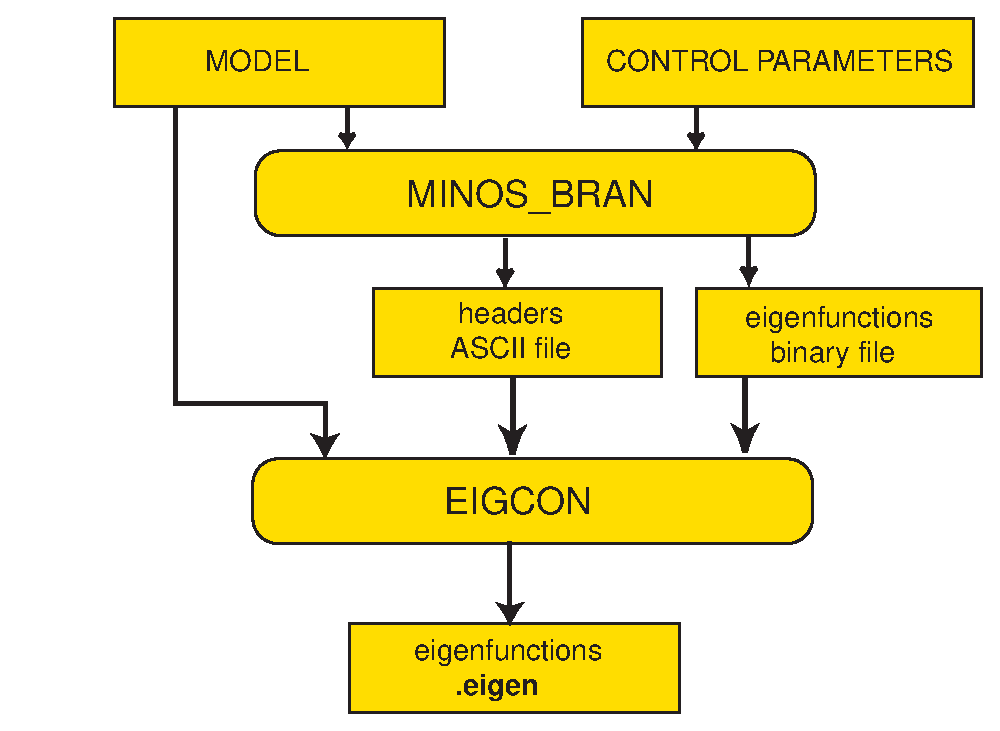
\includegraphics[width=5in]{Figures/Fig1}
\caption{Summary of information flow through the eigenfunction system of
programs comprising {\bf minos\_bran} and {\bf eigcon}.}
\label{fig:1}
\end{center}
\end{figure}

The program {\bf minos\_bran} is the work-horse of the {\bf Mineos} Package.
Given a 1D model of the earth and the normal mode band of interest (defined
in terms of a range of frequencies ({\it fmin, fmax}) and normal mode
indices ({\it nmin, nmax, lmin, lmax})), {\bf minos\_bran} computes and outputs the
eigenfunctions and eigenfrequencies of the model for spheroidal, toroidal,
or radial modes (optionally). The output from {\bf minos\_bran}
is in an informally defined pair of files, one an ascii file containing
the input model and output normal mode parameters and the other a binary file
containing the eigenfunctions from the free surface to the earth's center.
The size of the output depends on {\it fmax}, the highest
desired frequency, and the number of radial knots in the input model
file. If the desired frequencies extend to periods as short as
6 sec, the eigenfunctions and eigenfrequencies of more than 150,000 spheroidal 
and 100,000 toroidal modes will be computed if all dispersion branches
are chosen. 

The eigenfunctions themselves may be interesting to some users if sensitivity
kernels, for examples, are desired. The normalization of the eigenfunctions
that emerge from program {\bf minos\_bran} is discussed in section 3.

The program {\bf eigcon} repackages the eigenfunctions in two principal
ways. It, first, renormalizes the eigenfunctions and, second, truncates
the tabulation to extend only to a cut-off depth which is intended to be
the depth of the deepest earthquake considered. This truncation greatly
reduces the size of the eigenfunction file and speeds computation of the
Green functions. In addition, {\bf eigcon}
reformats the output eigenfunction file into a binary file that is
much more independent of computer architecture than that which emerges from
{\bf minos\_bran}.

The final output is represented more formally than the output from
{\bf minos\_bran}, based on the {\it .eigen} relation, which points
to the eigenfunction file on disk. The {\it .eigen} table is an extension of the CSS
database schema. 



\subsection{Synthetic Seismogram System of Programs}

%Figure 2
\begin{figure}
\begin{center}
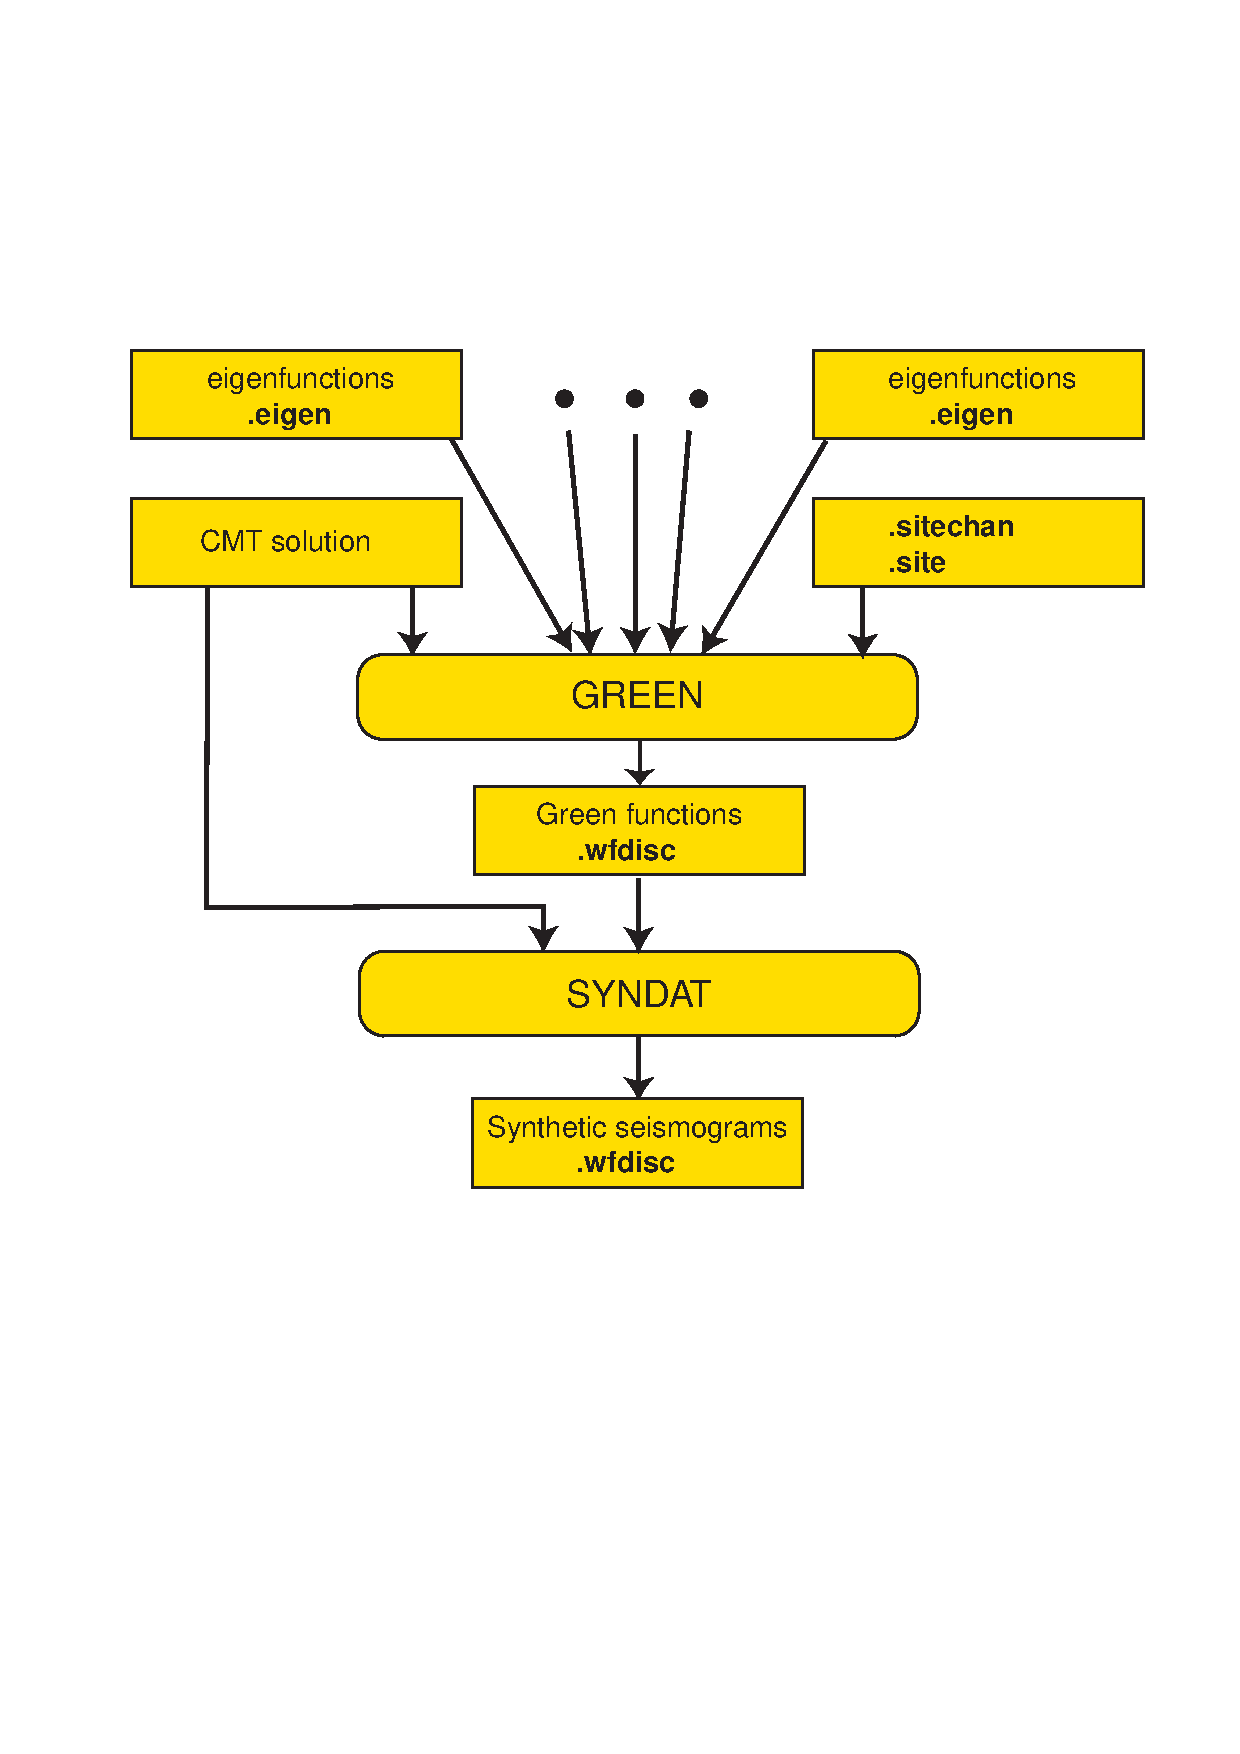
\includegraphics[width=5in]{Figures/Fig2}
\caption{Summary of information flow through the synthetic seismogram system of
programs comprising {\bf green} and {\bf syndat}.}
\label{fig:2}
\end{center}
\end{figure}

Synthetic seismograms are produced in two stages. In the first stage, program {\bf green}
computes Green functions and, in the second stage, program {\bf syndat}
transforms the Green functions to synthetic seismograms by convolving them with
a centroid moment tensor and input event half-rise time.

Program {\bf green} computes the Green function for an event at an input depth.
The primary input is the {\it .eigen} relation(s) output
from {\bf eigcon}. Typically, there may only be two {\it .eigen} files
input, one for spheroidal and another for toroidal modes. Radial modes
could constitute another input file. However, the input is sufficiently
flexible to allow the user to separate the input eigenfunctions into more
files, if desired. It is up to the user to ensure that the files contain
unique normal modes, however.
The stations and channels for which Green functions are produced by
program {\bf green} are driven by the input {\it .sitechan} table. The
{\it .site} table is also needed by {\bf green} to provide
the station coordinates. The {\it .sitechan} table, therefore,
must contain all and only those stations and channels desired by the user.
The user must strictly adhere to the format of these files. A natural way
to do this is to order a dataless (or data-full) SEED volume (for example
from the IRIS DMC) for the stations of interest, and run RDSEED or an Antelope product
(e.g., sd2de, seed2db) to convert to the two CSS tables. Event coordinates and depth
are contained in an unformatted, single lines file that we call {\it cmt\_event}.
This file must be created and input into program {\bf green} and {\bf syndat}.

The output of program {\bf green} is a {\it .wfdisc} file (in the CSS-3.0
data base schema) in which each row corresponds
to a given station:channel pair and points to the Green function on disk. Antelope
products can be used to view the Green functions in which each
station:channel set of six waveforms is multiplexed into
a single waveform.

Program {\bf syndat} convolves the Green functions pointed to
by the {\it .wfdisc} relation that emerges from {\bf green}
with the centroid-moment tensor and half-rise time of the chosen
event that is contained in file {\it cmt\_event}. The output
is a {\it .wfdisc} in which each row corresponds to a single
station:channel pair and points to the associated waveform on disk presented
in velocity ground units (nm/sec). Transfer functions to convert
to instrument counts for direct comparison with data are not part
of the package.




\subsection{Getting Started}

There are examples for running the four programs in section 10.
In addition, to help the user get started, the standard installation comes with several
input files.

\begin{description}
\item {\bf Model files}. Four model files are presented: {\bf prem\_noocean.txt, prem\_ocean.txt,
NRussia.txt, CPacific.txt}. The first two are for PREM, one with an ocean and the other
in which the ocean has been filled with solid crust. The other two model files are
a continental and an ocean point, in N. Russia and the C. Pacific, respectively. The model in the
latter two cases is the CU-Boulder 3-D model in the top 400 km, a 3-D model from Harvard 
through the rest of the mantle, underlain by PREM in the core, presented on a 2x2 deg
grid world-wide.
\item {\bf Eigenfunction files}. Output from {\bf eigcon} is presented for the
1D model PREM without an ocean. There are spheroidal and toroidal files. For
spheroidal modes, there is {\bf prem\_noocean\_S.eigen}
with the associated eigenfunction file that's contained in the directory {\bf
prem\_noocean\_S.eigen.dat},
simply called {\bf eigen}. Similarly, for toroidal modes there is {\bf prem\_noocean\_T.eigen}
and directory {\bf prem\_noocean\_T.eigen.dat}.
Eigenfunctions are computed with the following characteristics:
(fmin, fmax) = (0, 125.0 mHz), (nmin, nmax) = (1, 30), (lmin, lmax) = (1, 1631). This
produces all toroidal and the vast majority of spheroidal modes up to 8 sec period. There
are about 28,000 spheroidal and 28,000 toroidal modes. Truncation depth of the eigenfunctions is 1000 km.
The eigen files for the spheroidal
and toroidal modes are about 52 and 22 Mb,
respectively.
\item {\bf Event files}. There is a single event file called {\bf china\_cmt\_event.txt} 
  that contains Harvard CMT information for an event in Southern China.
\item {\bf Station:Channel files}. Two sets of station:channel files are included: (1) 
{\bf long.site} and {\bf long.sitechan} and (2) {\bf short.site} and {\bf short.sitechan}. 
The ``long" files are a long list of about 150 stations and
the ``short" list is about 15 stations at various distances from the event S. China.
\end{description}


\subsection{Utilities}
Currently we provide four utilities: {\bf cucss2sac}, {\bf eigen2asc},
{\bf endi}, {\bf simpledit}, and {\bf creat\_origin}.
%
\begin{itemize}
\item {\bf cucss2sac} converts synthetic waveforms represented in CSS3.0 
  (i.e., {\it .wfdisc} relation pointing to binary formatted waveforms on disk) 
  into SAC or ASCII formatted waveform files. Note that seismological coommunity provides us
  with another CSS to SAC converters, and you may use them for your own risk. For example,
  for the SUN platform, the distribution set
  {\tt css2sac-3.0.3.tar.z} is 
  available from {\it http://www.iris.edu}. The utility from that
  site, however,  doesn't work under Linux or Windows platforms. 
  The bugs are fixed in the {\tt css2sac\_082006.zip} package which is 
  available from {\it http://www.sunrisear.com/download.html}.
\item{\bf eigen2asc} prints out on a standard output device  requested 
  eigenfunctions from {\it .eigen} relation (CSS3.0 extension). 
  The eigenfunctions might be requested by order numbers, (n, l), or by 
  (n, T). In second case {\bf eigen2asc} matches the
  order number l with the closest period to T. Output might be redirected 
  to file for further usage.
\item  {\bf endi} swaps order of words bytes in binary files. The length
  of word is any integer number, for example, 2, 4, 6, 16, etc. 
  {\bf endi} might be used for BIG\_ENDIAN-LOW\_ENDIAN
  binary data conversation. Note, that this program upgrades files in place.
\item  {\bf simpledit} is a simple filter program. It converts a manually 
  created (text editor) unformatted ascii file with station and
  channel information into CSS3.0 {\it .site} and {\it .sitechan} relation
  tables.
\item {\bf creat\_origin} is a shell script  that converts an event 
  file (e.g., {\bf china\_cmt\_event.txt}) into the CSS3.0 {\it .origin} 
  relation.
\end{itemize}
For more details see Section 7 of this Manual.


\section{{\bf Mineos} system requirements}
\begin{itemize}
\item 32-bit processor (64-bit is recommended).
\item Unix Operating System.
\item 512 MB of RAM.
\item FORTRAN 77 and C compilers. Currently, the {\bf Mineos} package was
tested under SunOS 5.7/f77/cc and under Linux RedHat/f77/g77.
\item At least 1 GB of available hard-disk space.
\item autoconf 2.59 or higher version and automake 1.8.4 or higher version.
This requirement is only for software developers.
\end{itemize}

\section {minos\_bran program}

{\bf minos\_bran} program produces the solution of the seismic normal mode
eigenvalue-eigenfunction problem.
The program evaluates the eigenvalues and eigenfunctions for radial, spheroidal (S) and
toroidal (T) modes. The model of the earth is  self-gravitating, spherically
symmetric, transversely isotropic, and attenuative. \\
\noindent {\bf minos\_bran} is written in the FORTRAN-77 language.
\subsection {Command line}

\noindent {\bf minos\_bran}

\noindent {\bf minos\_bran} $<$ {\it parameter\_file}

\noindent {\bf minos\_bran} $<<$ WORD \\
\noindent ........  \\
\noindent ........  \\
\noindent WORD

\noindent There are three different ways to start the {\bf minos\_bran} program:
\begin{itemize}
\item interactive dialog for setting input parameters;
\item single shell command with redirection of the standard input to the parameter
file {\it parameter\_file} containing exactly the same information and
in the same order as an interactive dialog - one answer per line;
\item direct shell script. In this case, the contents of the parameter file are 
directly included into the shell script between the delimiters ``WORD". See examples.
\end{itemize}

\noindent The parameter file consists of six lines:
\begin{description}
\item[Line 1:] {\it model\_file} \\
{\it model\_file} is the path to the 1-D input model file. Text string up to 
256 characters long.
\item[Line 2:] {\it out\_plain\_file} \\
{\it out\_plain\_file} is the path to the output ASCII file. The file contains a model
listing  and a summary of mode properties. Text string up to 256 
characters long.
\item[Line 3:] {\it out\_bin\_file} \\
{\it out\_bin\_file} is the  path to the output FORTRAN unformatted binary file.
The file is a collection of eigenfunctions in a binary representation. 
The file name ``none" is a special name. ``none" will suppress the calculation 
of eigenfunctions. Text string up to 256 characters long.
\item[Line 4:] {\it eps, wgrav} \\
Parameter {\it eps} controls the accuracy of the 
Runge-Kutta integration scheme. The relative accuracy of an eigenfrequency 
is a factor 2-3 times {\it eps}. {\it eps} also controls the precision with 
which a root is found and the minimum relative separation of two roots 
with the same angular order. It is safe to set $eps = 10^{-7}$ for periods
greater than 10 seconds. For periods between 5 and 10 seconds, it has to be
set to $10^{-12} - 10^{-10}$. {\it wgrav} is the frequency in millihertz (mHz)
above which gravitational terms are neglected - this gives about a factor 
of 3 increase in speed. {\bf Format:} unformatted.
\item[Line 5:] {\it jcom} \\
{\it jcom} is the type of oscillation.  $jcom=1$ for radial modes, $=2$ for
toroidal modes, $=3$ for spheroidal modes, and $=4$ for inner core toroidal
modes. {\bf Format:} unformatted.
\item[Line 6:] {\it lmin, lmax, wmin, wmax, nmin, nmax} \\
$lmin,\; lmax$ define the range 
of angular orders $l$ to be computed. For radial modes, $jcom=1$,
$lmin,\; lmax$ are read in but are not used. $wmin,\;  wmax$
define the frequency range to be computed (in milli-Hertz). $nmin,\;nmax$ 
specify the range of dispersion branch numbers $n$ to be computed. $n = 0$ is the 
fundamental mode. {\bf Format:} unformatted.
\end{description}
%
% Input data
%
\subsection {Input data}

\textbf{\large \emph{model\_file.}} The model file is a plain ASCII file that may be
either given in tabular or polynomial form. The first two lines in the model file 
are common. The rest of the file depends on the setting and file type. 
A more detailed description of the model file is:
\begin{description}
\item[Line 1:] {\it title} \\
Any text up to 80 characters long.
\item[Line 2:] {\it ifanis, tref, ifdeck} \\
$ifanis=1$ for an anisotropic (transversely isotropic)
model, $=0$ for isotropic. $tref$ is the reference period (seconds) of the
model for the physical dispersion correction. If $tref \leq 0$ no correction is made.
The parameter $ifdeck$ defines the type of model.
If $ifdeck=1$, the model is presented in tabular form. If $ifdeck=0$, the
model is presented as a polynomial.
\end{description}
%
% Tabular model
%
{\large\it Tabular Setting,} {\it $ifdeck=1$}.
\begin{description}
\item[Line 3:] {\it N, nic, noc} \\
$N$ is the number of model knots and $N \leq 350$. $nic$ is the 
index of the solid side of the inner core boundary (ICB). $noc$ is the index of the
fluid side of the mantle core boundary (MCB). 
%Note that $n$ must be $\leq 223$. (mhr)
{\bf Format:} unformatted.
\item[Lines 4$\;-\;(N+3)$:] {\it r, rho, vpv, vsv, qkappa, qshear, vph, vsh, eta} \\
Each line describes the model parameter set for a single knot at radius $r$. 
Note that each knot has an integer index starting from 1, where the index is
equal to the line number minus 3. The discontinuity interfaces are
defined by a pair of knots at the same radius. \\
The line fields are:
\begin{itemize}
\item[{\it r}] - radius of the knot in meters (m). {\bf minos\_bran}
truncates the fractional part of radius, so a layer with thickness less that 1 m 
does not make any sense. Introducing thin layers (less than 1 m) leads to 
creating additional interfaces. If the model includes a surface liquid layer,
it must be a single layer without intermediate knots.
Radius starts from zero (index$=1$) and ends at the free surface,
growing from the center of the earth outward.
\item[{\it rho}] - density, ($\rm kg/m^3$)
\item[{\it vpv}] - velocity of vertically polarized P wave, (m/s)
\item[{\it vsv}] - velocity of vertically polarized S wave, (m/s)
\item[{\it qkappa}] - compressional Q
\item[{\it qshear}] - shear Q
\item[{\it vph}] - velocity of horizontally polarized P, (m/s)
\item[{\it vsh}] - velocity of horizontally polarized S, (m/s)
\item[{\it eta}] - transversely isotropic model parameter
\end{itemize}
If the model is isotropic, $ifanis = 1$ and {\bf minos\_bran} reads and changes
the values of {\it vph, vsh} and {\it eta} field in the following way:
$ vph=vpv,\;vsh=vsv$, and $eta=1$.
If both $qkappa$ and $qshear$ are equal to zero, the $Q$ model is not specified for the
knot and no correction for attenuation is made.\\
{\bf Format:} (f8.0, 3f9.2, 2f9.1, 2f9.2, f9.5)
\end{description}
%
% Polynomial model
%
{\large\it Polynomial Setting,} {\it $ifdeck=0$}.
\begin{description}
\item[Line 3:] {\it nreg, nic, noc, rx} \\
$nreg$ is the number of regions in the model, $nic$ and $noc$ have the same meaning
as for the tabular model, $rx$ is the normalizing radius for the polynomials.
$rx$ is given in (km) and it is usually 6371 km. {\bf Format:} unformatted.
\item[Line 4:] {\it nlay,r1,r2} \\
$nlay$ is the number of levels (layers) to be used in the region extending
from radius $r1$ to $r2$, $r1$ to $r2$ are  in (km). {\bf Format:} unformatted.
%
\item[Lines 5-9 or 5-12:] Lines 4-9 or 4-12 must be repeated $nreg$ times.
Lines 4-9 must be repeated for the isotropic model and lines 4-12
for the anisotropic model. Each line consists of five
coefficients $a_0,\;a_1,\;a_2,\;a_3,\;a_4$ for the fourth order polynomial 
$P(x)=a_0+a_{1}x+a_{2}x^2+a_{3}x^3+a_{4}x^4$, where, $x=r/rx$.
A set of 5 or 8 polynomials is used for interpolating the model parameters:
density, velocities, etc.,
as a function of normalized radius inside the region defined by line 4.
{\bf Format:} (5f9.5). More detail:
\item[Line 5:] Coefficients for density $rho$, ($\rm g/cm^3)$
\item[Line 6:] Coefficients for $vpv$, ($\rm km/s)$
\item[Line 7:] Coefficients for $vsv$, ($\rm km/s)$
\item[Line 8:] Coefficients for $qkappa$
\item[Line 9:] Coefficients for $qshear$
\item[] Three next lines must be added for an anisotropic model.
\item[Line 10:] Coefficients for $vph$, ($\rm km/s)$
\item[Line 11:] Coefficients for $vsh$, ($\rm km/s)$
\item[Line 12:] Coefficients for $eta$
\end{description}

\subsection {Output data}
{\bf minos\_bran} outputs an ASCII listing file and a FORTRAN unformatted
binary file. The first file contains the model table and the normal mode properties 
and the second contains the eigenfunctions.

\noindent \textbf{\large \emph{out\_plain\_file.}}
The file consists of two parts:
\begin{description}
\item[Part 1:] Model table. The model output is always in tabular form.
If the input model is in tabular form, the output model is just a 
copy except that knots are given indices and
columns are placed in a different order. For an isotropic model, $vph$ 
will be replaced on $vpv$,  $vsh$ on $vsv$, and $eta=1$.
If the input model is in polynomial form,
the model is converted to tabular form by interpolation across
region layers. For each region, the program constructs $nlay+1$ knots with a
constant step in radius.
The total number of knots $N$ is equal to $nreg \cdot (nlay+1)$.
Lines from the beginning of the file look as follows:
\begin{description}
\item[Lines] 1-5: Contains the model $title$, reference period $tref$,
header for the model table, and empty lines. {\bf Format:} no format.
\item[Lines] $6\;-\; (N+5)$: {\it index, r, rho, vpv, vph, vsv, vsh, 
eta, dshear, qkappa}\\
where $index$ is the knot number, starting from 1. The content of the 
remaining fields is described in section 3.2. {\bf Input data}. \\
{\bf Format:} (3x, i3, f12.1, 5f12.2, f12.5, 2f12.2)
\item[Lines] $N+6 \div \; N+11$: Contains text messages with Runge-Kutta
precision integration, gravity cut off frequency, empty lines, and the header
for the normal mode properties table (totaling 6 lines).\\
{\bf Format:} free.
\end{description}
\item[Part 2:] Mode properties. For a fixed radial order number $n$ and 
angular order $l,$ {\bf minos\_bran} computes the eigenfunctions (stored
separately) and the scalar parameters (properties): eigenvalue (frequency),
phase and group velocities, $Q$ and ratio of kinetic to potential energy.
These scalar parameters are stored in the the normal mode properties table. Each row
(line) in this table gives the properties for the current $n$ and $l$.
Lines following the first part look as follows:
\begin{description}
\item[Lines] $(N+12)\;-$ end: {\it norder, typeo, lorder, phvel, freq, per, grvel, Q, raylquo,} \\
where,
\begin{itemize}
\item[{\it norder}] - mode radial order number $n$
\item[{\it typeo}] - type of oscillation (single character): s - spheroidal, t - toroidal, c - inner
core toroidal
\item[{\it lorder}] - mode angular order number $l$
\item[{\it phvel}] - phase velocity, (km/s)
\item[{\it freq}] - frequency (eigenvalue), (millihertz,mHz)
\item[{\it per}] - period, per = 1000/freq, (sec)
\item[{\it grvel}] - group velocity, (km/s)
\item[{\it Q}] - shear Q
\item[{\it raylquo}] - ratio of kinetic to potential energy
minus 1 which should be small (of order $eps$), if the eigenfunction is
accurate and if there are enough radial knots in the model to allow
quadratures to be done accurately. (You will probably see some degradation
in this parameter for strongly exponential modes such as Stoneley modes ). \\
\end{itemize}
{\bf Format:} (i5, a2, i5, 6g16.7)
\end{description}
\end{description}
\noindent \textbf{\large \emph{out\_bin\_file.}} This is a fixed record length
binary encapsulated file. The file is not portable, which means that the type
of encapsulation strongly depends on the compiler. For example, if the file
was created on a SUN platform by the f77 compiler, it cannot be read by a progam
created by the g77 compiler on the same platform. To avoid this inconvenience,
the program {\bf eigcon} removes encapsulation and creates a binary file
portable between different languages and platforms. \\
{\bf minos\_bran} outputs each  et of the eigenfunctions with a single write 
statement\t:
\begin{quote}
\texttt{real*4 abuf(nvec)} \\
\texttt{.....} \\
\texttt{write(ioeig) (abuf(i),i$=$1,nvec)} 
\end{quote}
where nvec is $5+6*N$ words long for spheroidal modes and $5+2*N$ words long 
for other modes. The first five words of abuf are $n,l,\omega, Q$, and
group velocity $C_g$. The rest of \texttt{abuf} contains eigenfunctions and their
derivatives by radius - 
$U$(1..N), $U^\prime$(1..N), $V$(1..N), $V^\prime$(1..N),
$P$(1..N), $P^\prime$(1..N) for spheroidal modes and
$W$(1..N), $W^\prime$(1..N)
for other modes. Here, $U$ is the eigenfunction for the vertical spheroidal (S) component,
$V$ for the horizontal S component, $P$ is the gravitational potential. $W$ is the
common notation for modes other than S.\\
Eigenfunctions are stored in normalized form.
The normalization of eigenfunctions is given by 
\[       \omega^2 \int_0^{r_n} \rho(r)\; W^{2}(r)r^{2}\;dr = 1 \]
for toroidal modes and
\[       \omega^2 \int_0^{r_n} \rho(r)\; [U^{2}(r)+V^{2}(r)]r^{2}\;dr = 1 \]
for spheroidal modes. \\
Note that $r, \omega, \rho, V, U, W$ in the two formulas above are normalized such 
that a density of $\rho_n=5515$ $\rm kg/m^3$ is 1,
$\pi g$ is 1, where, $G$ is the gravitational constant $G=6.6723\cdot 10^{-11}$
$m^{3}/kg/s^2$, 
and the radius $r_n$ of the free surface is 1. These normalizations result in:
\begin{center}
\begin{tabular}{rl}
acceleration normalization: & $a_n=10^{20}/(\rho_n r_n^4)$; \\
velocity normalization:     & $v_n=r_n\;(\pi G\rho_n)^{-1/2}$; \\
frequency normalization:    & $\omega_n=v_n/r_n$; \\
radius normalization:       & $r_n$. \\
\end{tabular}
\end{center}

\subsection {Messages}
Program {\bf minos\_bran} prints out on the standad output dialog
messages only. See an example in section 10.1 (Interactive dialog).

%1. \texttt{in remedy with start level :   ??}

\section{eigcon program}

{\bf eigcon} program makes postprocessing of the {\bf minos\_bran} results and
creates the {\it .eigen} relation table in {\it dbname.eigen},
where {\it dbname} is the database name. 
The program creates a directory called {\it dbname.eigen.dat} in the same directory
where the file {\it dbname.eigen} is located. Under {\it dbname.eigen.dat}
it creates a binary file with a fixed name, {\it eigen}, for storing
the eigenfunctions. This binary file consists of segments with a
fixed length - one segment per eigenfunction.
The {\it eigen} binary file is a portable file. Unlike
the {\bf minos\_bran} binary file it does not have any encapsulation and
can be
easily treated by programs written in various high level languages 
such as C, C++, Perl, etc.
Access to a segment is provided through the {\it .eigen} relation table, namely,
by referencing the path, length,  byte offset, and by type of data. 
The {\it .eigen}
relation table, Section 8, has the structure of an external database file
and can be easily incorporated into relational databases such as
ORACLE, Postgress, MySql, etc.

\subsection {Command line}

\noindent {\bf eigcon}

\noindent {\bf eigcon} $<$ {\it parameter\_file}

\noindent {\bf eigcon} $<<$ WORD \\
\noindent ........  \\
\noindent ........  \\
\noindent WORD

\noindent There are three different ways to start the {\bf eigcon} program:
\begin{itemize}
\item interactive dialog for setting input parameters;
\item single shell command with redirection of the standard input from a parameter
file {\it parameter\_file} containing exactly the same information and
in the same order as in the interactive dialog - one answer per line;
\item direct shell script. In this case, the contents of the parameter file are
directly included in the shell script between delimiters ``WORD". See examples.
\end{itemize}
\noindent The parameter file consists of six lines:
\begin{description}
\item[Line 1:] {\it jcom} \\
{\it jcom} is the type of oscillation.  $jcom=1$ for radial modes, $=2$ for
  toroidal modes, $=3$ for spheroidal modes, and $=4$ for inner core toroidal
  modes. \\
  {\bf Format:} unformatted.
\item[Line 2:] {\it model\_file} \\
  {\it model\_file} is the path to the 1-D input model file. Text string up to
  256 characters long.
\item[Line 3:] {\it max\_depth}\\
  {\it max\_depth} is the depth to cut all output eigenfunctions (in km). All output
  values exists in the interval $[r_n,r_n - max\_depth]$ only. $r_n$ is the radius
  of the  free surface in km. \\
  {\bf Format:} unformatted.
\item[Line 4:] {\it in\_plain\_file} is the path to the input ASCII file. 
  The file is the output model listing  {\it out\_plain\_file} of the
  program {\bf minos\_bran}. See section 3.3.
  Text string up to 256 characters long.
\item[Line 5:] {\it in\_bin\_file} \\
  {\it in\_bin\_file} is the  path to the input FORTRAN binary unformatted file,
which was produced by the program {\bf minos\_bran}.
 See section 1.3.
\item[Line 6:] {\it dbname} \\
  {\it dbname} is the path to the output database name. The path is a string up to 256
  characters long. The path should not
  end with a backslash, ``/". The part of string after the last ``/" or from the
  beginning of the string, if string does not have ``/" at all, is the
  data base name. The data base name must be at least one character long.
\end{description}
%
% Input data
%
\subsection {Input data}

\textbf{\large \emph{model\_file.}} See description in Section 3.2, 
\textbf{\emph{model\_file}}.

\noindent \textbf{\large \emph{in\_plain\_file.}}
This file has been created by {\bf minos\_bran} as an output file.
See description of the file in Section 3.3, \textbf{\emph{out\_plain\_file}}.
Actually, {\bf eigcon} uses only normal mode properties from this file to create
some part of {\bf .eigen} relation table.

\noindent \textbf{\large \emph{in\_bin\_file.}}
This file has been created by {\bf minos\_bran} as an output file.
See description of the file in Section 3.3, \textbf{\emph{out\_bin\_file}}.

\subsection {Output data}

As mentioned above, {\bf eigcon} creates three objects in the file system:
a relational table \\
{\it dbname.eigen}, a directory {\it dbname.eigen.dat}, and a
binary file {\it dbname.eigen.dat/eigen}.

\textbf{\large \emph{dbname.eigen}} file format is described in Section 8 as
the relation table {\it .eigen}. Each line of this file describes the modal
properties of a single eigenfunction and references the binary data
segment in the {\it dbname.eigen.dat/eigen} file.

\textbf{\large \emph{dbname.eigen.dat/eigen}} binary file consists of segments.
Each segment stores normalized eigenfunctions for a single normal mode ($n,l$). 
It consists of words 4 bytes long containing real*4 or integer*4 variables
in the internal computer
format. The field {\it datatype} in {\it .eigen} describes numeric memory
storage data (byte order). There are two common byte orders
for most of computer architectures:
BIG\_ENDIAN (straight order 1-2-3-4) and LOW\_ENDIAN (reverse order 4-3-2-1).
BIG\_ENDIAN is used by SUNS and RISC-oriented platforms, and LOW\_ENDIAN is 
used by PC, VAX and DEC hardware. {\bf eigcon} automaticaly detects the byte order
and places the text strings ``t4" (BIG\_ENDIAN) or ``f4" (LOW\_ENDIAN) into the
{\it datatype} field in the {\it .eigen} relation.

Each segment is logically divided into two parts -  the header and the body. \\
{\bf \emph{The header.}} This part of the segment stores   scalar 
parameters  and normalization coefficients
for the modal properties.
\begin{quote}
\begin{description}
\item[{\bf word 1:} {\tt integer*4}, $n$] - normal mode radial order number $n$. Must
  be equal to {\it norder} in the referencing {\it .eigen} relation.
\item[{\bf word 2:} {\tt integer*4}, $l$] - normal mode angular order 
(harmonic degree) number $l$. Must
  be equal to {\it lorder} in the referencing {\it .eigen} relation.
\item[{\bf word 3:} {\tt real*4}, $\omega$] Normal mode frequency (eigenvalue) in
  physical units rad/s, \mbox{$\;\omega=2\pi/per$}. $per$ is the period field in the
  {\it .eigen} relation.
\item[{\bf word 4:} {\tt real*4}, $q$] - part of the exponential term in the
  attenuation
  expression, \mbox{$e^{-qt}$}, \mbox{$q=0.5*\omega/Q$}, rad/sec.
\item[{\bf word 5:} {\tt real*4}, $r_n$] - the radius normalization coefficient 
  in meters, equal to the radius of the model's free surface.
\item[{\bf word 6:} {\tt real*4}, $v_n$] - the velocity normalization 
  coefficient, $v_n=r_n\;(\pi G\rho_n)^{-1/2}$, where,
$G$ is the gravitational potential constant 
($G=6.6723\cdot 10^{-11}$ $\rm m^3/kg/s^2$),
$\rho_n$ is the density normalization coefficient ($\rho_n=5515$ $\rm kg/m^3$).
The circular frequency normalization coefficient $\omega_n$ is given by
$\omega_n=v_n/r_n$.
\item[{\bf word 7:} {\tt real*4}, $a_n$] - the acceleration normalization 
  coefficient, \mbox{$a_n=10^{20}/(\rho_n r_n^4)$}.
\end{description}
\end{quote}
%
\noindent {\bf \emph{The body - eigenfunction grid.}}
%
\begin{quote}
\begin{description}
\item[{\bf word 8$\;-\;$end:}] {\tt real*4}, $E(nrow,ncol)$ - matrix 
  of $nrow$ rows and $ncol$ columns to store the normalized eigenfunctions. 
  The first column is radius. The other columns are the
  eigenfunctions.
  The number of eigenfunctions depends on modal type. For spheroidal
  modes, it should be 7 columns ($r,\;U,\;U^\prime,\;V,\; V^\prime,\;P,
  \;P^\prime$), for toroidal and others, it should be 3 columns ($r,\;W,\;W^\prime$).
  The matrix is stored in segments by the second index, by columns.
\end{description}
\end{quote}

\noindent Note that {\bf eigcon} performs an additional eigenfunction
normalization. Eigenfunctions for toroidal and the horizontal  
part of spheroidal modes are divided by $(l(l+1))^{1/2}$.
This is done in accordance with theory developed by
Woodhouse \& Dahlen (1978).
The new normalization of eigenfunctions is given by
\[       \omega^2 \int_0^{r_n} \rho(r)\; l(l+1)\;W^{2}(r)r^{2}\;dr = 1 \]
for toroidal modes and
\[       \omega^2 \int_0^{r_n} \rho(r)\; [U^{2}(r)+l(l+1)\;V^{2}(r)]r^{2}\;dr = 1 \]
for spheroidal modes.
%
\subsection{Messages}
Program {\bf eigcon} prints out on the standad output 
device the following messages:

\noindent \textbf {\emph{Dialog messages}}. Copy of input/output dialog
or parameter file in dialog form. For example,

\noindent \texttt {spheroidals (3) or toroidals (2) or radial (1) or  \\
inner core toroidals (4) modes \\
\emph{3} \\
enter name of model file \\
\emph{model\_PREM.txt} \\
enter max depth [km] : \\
\emph{40.} \\
enter name of minos\_bran output text file \\
\emph{PREM\_S} \\
minos\_bran output binary unformatted file name \\
\emph{ePREM\_S} \\
enter path/dbase\_name or dbase\_name to store eigenfunctions: \\
\emph{test\_S} } 

\noindent \textbf {\emph{Info and error messages}}. 

\noindent 1. \texttt{============= Program eigcon ====================} 
\begin{quote}  
Info message. Shows that program {\bf eigcon} starts.
\end{quote}
\noindent 2. \texttt{eigcon: n,nstart,nrad = nnn, mmm, kkk}
\begin{quote}  
Info message. {\tt nnn} is the total number of nodes  of eigenfunction,
{\tt mmm} is the number of staring node after cutting eigenfunction by depth,
and {\tt kkk} is the rest number of nodes after cutting.
\end{quote}
\noindent 3. \texttt{ERR001: eigcon: Input plane and binary files differ: nn, ll, n, l }
\begin{quote}  
\noindent Order numbers of some eigenfunctions {\tt nn} and {\tt ll} in the text 
file differ from the numbers {\tt n, l} in the binary data segment. 
Program is terminated. Check {\it .eigen} relation or create it again.
\end{quote}
\noindent 4. \texttt{ERR002: eigcon: Unknown jcom nnn}
\begin{quote}  
\noindent Error message. The parameter {\tt jcom} with value {\tt nnn} 
is out of range.  Program is terminated. Provide {\tt jcom} with right value.
\end{quote}
\noindent 5. \texttt{ERR003: eigcon: jcom = nnn does not fit mode sss}
\begin{quote}  
\noindent Error message. Impossible combination of jcom and mode. For example,
jcom=2 (toroidal modes) can not used together with {\bf minos\_bran} 
unformatted file for spheroidal modes.
Program is terminated. Provide right jcom and unformatted file.
\end{quote}
\noindent 6. \texttt{ERR004:eigcon: Wrong minos\_bran output text file}
\begin{quote}  
\noindent Error message. Probably the {\bf minos\_bran} plain file was edited.
Never change this file. Program is terminated. Rerun {\bf minos\_bran} again
to create proper plain file.
\end{quote}

\section{green program}

{\bf green} program computes for a single event and a given
set of stations, the Green functions. For each station,
a station-channel list specifying the orientation of the sensors must
be input.
The program can optionally compute Green functions (a) for
the Z component alone, (b) for 3-components  with the standard ZNE sensor
orientation (see Appendix C), or (c) for 3-components with the Z component 
directed ''up" and two orthogonal horizontal components oriented 
arbitrarily. To set up station information, it is necessary to create 
a flat file database consisting of the two relations
{\it .site}, and {\it .sitechan} in the CSS 3.0 database format.
It is preferable to create the relations by a program, for example, by
IRIS's {\bf rdseed} program or by selection from a global database.
Other input includes the eigenfunctions which are collected from various databases
containing {\it .eigen} relations for spheroidal or toroidal modes. 
For each sensor, {\bf green} computes and stores in an output {\it .wfdisc} relation
six Green functions, one per moment tensor component. 

\subsection {Command line}

\noindent {\bf green}

\noindent {\bf green} $<$ {\it parameter\_file}

\noindent {\bf green} $<<$ WORD \\
\noindent ........  \\
\noindent ........  \\
\noindent WORD

\noindent There are three different ways to start the {\bf green} program:
\begin{itemize}
\item interactive dialog for setting the input parameters;
\item single shell command with redirection of the standard input to a parameter
file {\it parameter\_file} containing exactly the same information and
in the same order as in the interactive dialog - one answer per line;
\item direct shell script. In this case, the contents of the parameter file are
directly included in the shell script between the delimiters ``WORD". See examples.
\end{itemize}
\noindent The input parameter file consists of six lines:
\begin{description}
\item[Line 1:] {\it in\_dbname } \\
{\it in\_dbname } is the input database name for the {\it .site} and {\it .sitechan} relations. \\
  {\bf Format:} Any string up to 256 characters long.
\item[Line 2:] {\it db\_list} \\
  This is the path to the file defining  the list of database names containing
the eigenfunctions - one
  name per line. 
  Each name refers to the database in which the {\it .eigen} relation resides. \\
  {\bf Format:} Any string up to 256 characters long.
\item[Line 3:] {\it cmt\_event}\\
  This is the path to the file with the CMT solution for a single event. It includes 
  the CMT location, the seismic moment tensor components, the scalar moment, the focal 
  planes, the source half duration time, and the output time step of the synthetic 
  seismograms. \\
  {\bf Format:} Any string up to 256 characters long.
\item[Line 4:] {\it fmin, fmax} \\
  {\it fmin, fmax} define the frequency range to be selected from the input
  eigenfunction databases. All modes with frequences out of this range are 
  rejected. \\
  {\bf Format:} Unformatted.
\item[Line 5:] {\it nsamples} \\
  This is the number of samples in the synthetic seismograms. All synthetic 
  seismograms start from the source time. \\
  {\bf Format:} Unformatted.
\item[Line 6:] {\it out\_dbname} \\
  This is the output database name including only the {\it .wfdisc} relation for 
  unit Green functions. Each row of the {\it .wfdisc} relation refers to the binary 
  file with 6 multiplexed Green functions; i.e., one tensor component. \\
  {\bf Format:} Any string up to 256 characters long.
\end{description}
%
% Input data
%
\subsection {Input data}

\textbf{\large \emph{in\_dbname.}} 
  This database must exist and must include
  {\it .site} and {\it .sitechan} relations. 
  The {\it .sitechan} relation provides the station-channel list used
by the program. Using these relations, the
  {\bf green} program defines for each station 
  a certain number of channel groups. Each group consists of the single 
  Z-component channel or a triple of channels (Z-component, and two horizontal 
  components with sensor directions defined by the {\it hang} field in the
sitechan relation).
  Before grouping, the {\bf green} program sorts the {\it .sitechan} file
by its ({\it sta, chan}) fields. After sorting, it also removes all duplicate 
  rows (equal station and channel code). Note that the channel field,
  {\it chan}, in the {\it .sitechan} relation is a
  three-character channel name following the SEED format convention. 
  The first two characters define the type of channel (e.g., BH, LH, etc.)
unique, for each
  station's group.
  The third character must be the component name: Z (upper case, for vertical) 
  and other symbols (any case, for the horizontals). \\
\\
\textbf{\large \emph{db\_list.}} This file allows 
  joining an unlimited number of {\bf eigcon} outputs for spheroidal, toroidal, or
  radial modes. The single requirement is that intersection between these
files is null. Each desired eigenfunction must be present and unique in
  some {\bf eigcon} output. \\
\\
\textbf{\large \emph{cmt\_event.}} This file consists of a single line with the 
  following fields:  \\
\begin{quote}
{\it evid, year, jday, hour, min, sec, lat, lon,
  depth, step, halfd, }\\
  $M_0$, $M_{rr},\;M_{\theta \theta},\;M_{\varphi\varphi},\;
  M_{r \theta},\; M_{r \varphi},\; M_{\theta\varphi},$ \\
  $M_{n},$ {\it strike1, dip1, slip1, strike2, dip2, slip2,}.
\end{quote}
where, 
\begin{quote}
\begin{description}
\item[{\it evid}] is the event identifier, 8 characters long 
\item[{\it year}] is the event year of form {\bf yyyy} 
\item[{\it jday}] is the event day starting from the beginning of the year 
\item[{\it hour}] is the event hour
\item[{\it min}] is the event minutes
\item[{\it sec}] is the event seconds with decimal fraction
\item[{\it lat}] is the event geographical latitude, (degree)
\item[{\it lon}] is the event geographical longitude, (degree)
\item[{\it depth}] is the event depth, (km)
\item[{\it step}] is the time step for Green functions and seismograms, sec
\item[{\it halfd}] is the source half time duration, sec
\item[$M_0$] is the scalar tensor moment, (dyn$\cdot$cm)
\item[$M_{rr},$] $M_{\theta \theta},\;M_{\varphi\varphi},\;
M_{r \theta},\; M_{r \varphi},\; M_{\theta\varphi}$ are moment 
  tensor components normalized by the coefficient $M_n$.
\item[$M_n$] is the normalization coefficient for the tensor components,
(dyn$\cdot$cm)
\item[{\it strike1,}] {\it dip1, slip1} are the first fault plane
  solution, (degree)
\item[{\it strike2,}] {\it dip2, slip2} are the second fault plane
  solution, (degree)
\end{description}
\end{quote}

\subsection {Output data}

\textbf{\large \emph{out\_dbname.}} Program {\bf green} creates a {\it .wfdisc}
relation in database {\it out\_dbname} and a  multiplexed binary file contained
the Green function waveforms.
The binary file contains six Green functions in  an order corresponding to the
tensor components:
$M_{rr},\; M_{\theta \theta},\;M_{\varphi\varphi},\;
M_{r \theta},\; M_{r \varphi},\; M_{\theta\varphi}$. The total length,
$nsamp$, of the file is equal to $6*nsamples$. 

\subsection{Messages}
Program {\bf green} prints out on the standard output
device the following messages:

\noindent \textbf {\emph{Dialog messages}}. Copy of input/output dialog
or parameter file in dialog form. For example,

\noindent \texttt {enter path to db with sta \& stachan: \\
\emph{RDSEED\_rdseed} \\
enter name of file within list of nmodes db: \\
\emph{db\_list} \\
enter input CMT file name: \\
\emph{cmt\_event} \\
min and max frequencies to be considered (mHz) : \\
\emph{0.  260.} \\
enter \# pts in greens fns .le.  30000 : \\
\emph{4000} \\
enter Green functions output db file name: \\
\emph{green}}

\noindent \textbf {\emph{Warning, error, and info messages}}.

\noindent 1. \texttt{ ============= Program green ====================}
\begin{quote}
Info message. Shows that program {\bf green} starts.
\end{quote}
\noindent 2. \texttt{WARNING: green: \# of points in Green functions is stripped to nnn}
\begin{quote}
Warning message. The number of requested points for the Green functions
exceeds the maximum allowed value {\tt mseis}. The number is reduced to {\tt mseis}
and the program continues to run. To increase the maximum value, change  {\tt mseis} to
a new bigger value in the {\tt green.h} header and recompile the {\bf green} program.
By default, {\tt mseis=30000}.
\end{quote}
\noindent 3. \texttt{WARNING: green: \# of channels is stripped to 3}
\begin{quote}
Warning message. Number of sensors (channels, components) in a group cannot 
be greater than 3.
Only the three first sensors are taken into account. 
\end{quote}
\noindent 4. \texttt{WARNING: green: \# of channels is stripped to 1}
\begin{quote}
Warning message. Number of sensors in a group cannot be equal to 2.
Only the first sensor is taken into account. 
\end{quote}
\noindent 5. \texttt{WARNING: green: Channel: \# 1 is not vertical. Sequence ignored}
\begin{quote}
Warning message. Channel with Z component must be the first in the group.
The group of channels is rejected.
\end{quote}
\noindent 6. \texttt{WARNING: green: Channel: \# nnn is not horizontal. Sequence ignored}
\begin{quote}
Warning message. Second and third channels in the group must be horizontal
components. nnn is the channel number in the group. The group of channels is rejected.
\end{quote}
\noindent 7. \texttt{ERR010: green: max l = nnn, must be .le. ml}
\begin{quote}
Error message. The max angular order number {\tt nnn} for some mode {\tt n}
exceeds the parameter {\tt ml} set up in the {\tt green.h} header.
Program is terminated.
To avoid the problem, make {\tt ml} bigger than {\tt nnn} in the {\tt green.h} header
and recompile the program. It is not recommended to make {\tt ml} greater than
10000, which leads to inaccuracy in computing the associated Legendre polynomials.
By default, {\tt ml = 6000}.
\end{quote}
\noindent 8. \texttt{ERR011:eigen: flat and bin indices are different}
\begin{quote}
Error message. Broken input {\it .eigen} relation. Program is
terminated. Check or create {\it .eigen} again.
\end{quote}
\noindent 9. \texttt{ERR012: green: \# sph. modes in band exceed max 
allowed number nnn}
\begin{quote}
Error message. The total number of spheroidal modes in the band exceeds the
maximum allowed
number of {\tt nnn}. Program is terminated. Increase parameter {\tt meig} in the
{\tt green.h} header and recompile the program. By default, {\tt meig = 200000}.
\end{quote}
\noindent 10. \texttt{ERR012: green: \# tor. modes in band exceed max allowed number nnn}
\begin{quote}
Error message. The total number of toroidal modes in the band exceeds 
the maximum allowed
number {\tt nnn}. Program is terminated. Increase parameter {\tt meig} in the
{\tt green.h} header and recompile the program. By default, {\tt meig = 200000}.
\end{quote}
\noindent 11. \texttt{green: \# sph. modes in band = nnn  must be .le. meig}
\begin{quote}
Info message. \texttt{nnn} is the total number of spheroidal modes in all
input databases. \texttt{meig} is the maximum allowed number of spheroidal modes.
\end{quote}
\noindent 12. \texttt{green: \# tor. modes in band = nnn  must be .le. meig}
\begin{quote}
Info message. \texttt{nnn} is the total number of toroidal modes in all
input databases. \texttt{meig} is the maximum allowed number of toroidal modes.
\end{quote}
\begin{description}
\item[13.] \texttt{green: evid date\&time lat = $\pm$dd.ddd, lon = $\pm$ddd.ddd}
\item[$\;\;\;\;\;$] \texttt{green:        source depth = ddd.d km}
\item[$\;\;\;\;\;$] \texttt{green: step =    d.ddd sec, nsamples =  ddddd}
\end{description}
\begin{quote}
Info message. This message outputs part of the {\it cmt\_event} file: 
event information, Green function's time step and number of samples. 
See description of the {\it cmt\_event} file in Section 5.2.
\end{quote}
\noindent 14. \texttt{green: Input dbname : xxxxx}
\begin{quote}
Info message. xxxxx is the name of the input database for the {\it .site} and 
{\it .sitechan} relations.
\end{quote}
\noindent 15. \texttt{green: Station: code     lat   lon , Channels: nnn}
\begin{quote}
Info message. This message specifies the station code, station coordinates, 
and number of components nnn for the selected group of sensors.
\end{quote}
\noindent 16. \texttt{green: Channel: \#  nnn  code   chan  hang vang}
\begin{quote}
Info message. This message specifies a separate sensor (channel) for
the group of sensors. nnn is the current number in the group, code is the
station code, chan is the channel name. hang (horizontal angle) and vang 
(vertical angle) are sensor orientation
in space. See {\it .sitechan} relation in Section 8.
\end{quote}
\noindent 17. \texttt{green: Epicentral Distance :    ddd.ddd}
\begin{quote}
Info message. ddd.ddd is the station-event distance in degrees.
\end{quote}
\noindent 18. \texttt{green: Azimuth of Source :    ddd.ddd}
\begin{quote}
Info message. ddd.ddd is the azimuth of a station to the source point.
in degree.
\end{quote}
\noindent 19. \texttt{green: Azimuth of Source :    ddd.ddd}
\begin{quote}
Info message. ddd.ddd is the azimuth of  the station to the source point
 in degrees.
\end{quote}
\noindent 20. \texttt{green:   nnn code    chan  date\&time  step   mmm}
\begin{quote}
Info message. This message informs about some attributes specifying the
Green functions. nnn is the global number of Green functions set, code is the
station name, chan is the channel name, date\&time is the event origin 
time, step is the Green function sampling step in seconds, and mmm is 
the total number of samples for the block of 6 Green functions. 
\end{quote}

\section{syndat program}

{\bf syndat} program makes synthetic seismograms by convolution
of Green functions ({\bf green} program output) with the
seismic moment tensor of the chosen event.

\subsection {Command line}
                                                                               
\noindent {\bf syndat}

\noindent {\bf syndat} $<$ {\it parameter\_file}

\noindent {\bf syndat} $<<$ WORD \\
\noindent ........  \\
\noindent ........  \\
\noindent WORD

\noindent There are three different ways to start the {\bf syndat} program:
\begin{itemize}
\item interactive dialog for setting input parameters;
\item single shell command with redirection of the standard input from a parameter
file {\it parameter\_file} containing exactly the same information and
in the same order as in the interactive dialog - one answer per line;
\item direct shell script. In this case, the contents of the parameter file are
directly included in the shell script between the delimiters ``WORD". See examples.
\end{itemize}
\noindent The parameter file consists of four lines:
\begin{description}
\item[Line 1:] {\it cmt\_event}\\
  This is the path to the file with the CMT solution for a single event. It must be the same
  {\it cmt\_event} file as used in the construction of the Green functions by the
 {\bf green} program. It uses part of the file
  defining the seismic moment tensor components, scalar moment, and focal planes. \\
  {\bf Format:} Any string up to 256 characters long.
\item[Line 2:] {\it in\_dbname } \\
{\it in\_dbname } is the input database name for the input Green functions. The {\it .wfdisc} relation of the
  {\it in\_dbname } database must be the output {\it .wfdisc} relation of the
  {\bf green} program. \\
  {\bf Format:} Any string up to 256 characters long. 
\item[Line 3:] {\it plane} \\
  This defines the method for introducing the moment tensor components.
  If $plane=0$, the tensor components come in directly from the {\it cmt\_event}
  file as is. If $plane=1$, the program takes the scalar moment and angles from
  focal plane 1 and computes the moment tensor components. For $plane=2$,
  the program computes the tensor components using the scalar moment and
  focal plane 2. \\
  {\bf Format:} Unformatted.
\item[Line 4:] {\it out\_dbname} \\
  This is the output database name for the {\it .wfdisc} relation for 
  synthetic seismograms. Each row of the {\it .wfdisc} relation refers to 
  a binary file with synthetic data in nm/sec. \\
  {\bf Format:} Any string up to 256 characters long.
\item[Line 5:] {\it datatype} \\
  This defines the type of synthetic data. If $datatype=0$ the 
  output synthetic waveforms are accelerograms in $nm/s^2$. This is 
  recommended native {\bf Mineos} output. If $datatype=1$ the
  output is velocity waveform in $nm/s$, and if $datatype=2$ the
  output is displacement in $nm$. This is done by additional
  conversation of accelerograms to velocity or displacement.
\end{description}
%
% Input data
%
\subsection {Input data}

\textbf{\large \emph{cmt\_event.}} See description in section 5.2. \\
\textbf{\large \emph{in\_dbname.}} {\it out\_dbname} database for the {\it .wfdisc}
relation from the  {\bf green} program. 
\subsection {Output data}
\textbf{\large \emph{out\_dbname.}} Database name for the final synthetic seismograms
referenced by the {\it .wfdisc} relation.


\section{The Utilities User's Manual}
\subsection{cucss2sac}
\noindent {\bf NAME}
\vred
\begin{itemize}
\vred
\item[]{\bf cucss2sac} - convert CSS 3.0 waveforms to SAC binary or ASCII files
\vred
\end{itemize}
\vred
\noindent {\bf SYNOPSIS}
\vred
\begin{itemize}
\vred
\item[] {\bf cucss2sac [-a [-n]] db\_name out\_SAC\_dir}
\vred
\end{itemize}
\vred
{\bf OPTIONS}
\vred
\begin{itemize}
\vred
\item[]    {\bf -a} - generate ASCII files
\vred
\item[]    {\bf -n} - suppress header output in ASCII files. Used together with {\bf -a} option.
\vred
\end{itemize}
\vred
{\bf DESCRIPTION}
\vred
\begin{quote}
\vred
{\bf cucss2sac} utility converts a CSS 3.0 {\it .wfdisc} relation into a set 
of SAC binary files or  ASCII files. Output files are stored in 
{\bf out\_SAC\_dir} directory. This program has been designed 
especially for the {\bf Mineos} package due to bugs in the standard IRIS 
{\bf css2sac} utility. {\bf cucss2sac} supports limited capabilities 
and is not a complete substitution of the standard {\bf css2sac} 
utility. For example, {\bf cucss2sac} only supports the CSS3.0 schema 
and two input CSS binary data formats: ``t4" (BIG\_ENDIAN, single 
precision floating point) and ``f4" ( LOW\_ENDIAN, single precision 
floating point). {\bf cucss2sac} converts CSS binary data ``as is" 
without any corrections or modifications. For the {\bf Mineos} package, 
{\bf cucss2sac} may be used for the conversation of Green functions 
or synthetic seismograms to binary SAC or ASCII files.

A CSS database {\bf db\_name} must include at least one file 
db\_name.wfdisc file containing CSS format information about the 
waveforms. It is also desirable to add to the database {\it .origin} and 
{\it .site} relation tables (files db\_name.origin and db\_name.site) 
to get a more complete SAC header.
Note that the {\it .origin} relation keeps information about event location 
and the {\it .site} relation keeps station locations. If {\it .origin} is present 
in the database, {\bf cucss2sac} uses only the first line from this 
file. In the case of ASCII output, all available parameters go to the
ASCII header - three lines in the beginning of the file. 
For example, output file for a synthetic seismogram looks as follows:

\texttt{EVENT:   2000(014)-23:37:10.800 947893030.80000 25.3900 101.4000 33.0000 \\
   STATION: ALE     LHE       82.5033  -62.3500  0.0000 \\
   DATA:    2000(014)-23:37:10.800  947893030.80000  8000 1.000000 \\
     0.0000000E+00   5.7025738E+00 \\
     1.0000000E+00   1.9508668E+00 \\
     2.0000000E+00  -4.1160989E+00 \\
     3.0000000E+00  -4.1094885E+00 \\
          ...... \\
          ...... \\
          ...... \\
     7.9970000E+03   1.5211651E+01 \\
     7.9980000E+03   2.7408613E+01 \\
     7.9990000E+03   3.5795624E+01}

where,
the \texttt{EVENT} line represents event information: origin time 
(human and epoch), latitude (deg), longitude (deg), and depth (km); 
the \texttt{STATION} line represents station information: station code,
channel name, latitude (deg), longitude (deg), and depth = 0; the 
\texttt{DATA} line represents data parameters: waveform 
starting time (human and epoch), number of samples, and sampling step 
(sec). The rest of the lines, the body, is two columns table. The first 
column represents relative time from the beginning of waveform in 
seconds and the second ones waveform samples in nm, nm/s or nm/s$^2$, 
according to the {\bf syndat} output format.

If the presence of the header is not desired, suppress it with option 
{\bf -n} (no header).

The output ASCII file format for the Green functions is different. 
The header is the same, but the body is a 7 column table. The first 
column is relative time, as before, and the other 6 columns are the 6 
unit Green functions ($G_{rr}, G_{\theta\theta}, G_{\varphi\varphi}, 
G_{r\theta}, G_{r\varphi}, G_{\theta\varphi}$) for the chosen 
component - vertical or some horizontal. The order of the components 
is the same as the order of the seismic moment tensor components 
$M_{ij}$ defined in the {\bf syndat} program. So, the corresponding 
synthetic seismogram S (IN ACCELERATION !!!, nm/s$^2$) is given by 
the formula

            \[ S = 10^{-18}\;\sum_{ij} G_{ij}\;M_{ij} \]

where $M_{ij}$ are given in dyne*cm for $ij = rr, \theta\theta,
\varphi\varphi, r\theta, r\varphi, \theta\varphi$.

NOTE: According to SAC complaince, event depth is stored in the SAC 
header in meters.
\end{quote}
\vred
{\bf EXAMPLES}
\vred
\begin{quote}
\vred
\textbf{cucss2sac Syndat Syndat\_SAC  \\
    cucss2sac green  green\_SAC \\
    cucss2sac -a Syndat Syndat\_ASC \\
    cucss2sac -a -n Syndat Syndat\_ASC\_NOHEADER} 
\vred
\end{quote}
\newpage
% EIGEN2ASC
\subsection{eigen2asc}
\noindent {\bf NAME}
\vred
\begin{itemize}
\vred
\item[] {\bf eigen2asc} - convert {\it .eigen} relation table to ASCII files
\vred
\end{itemize}
\vred
\noindent {\bf SYNOPSIS}
\vred
\begin{itemize}
\vred
\item[] {\bf eigen2asc [-n] nmin nmax lmin lmax db\_name out\_dir}
\vred
\end{itemize}
\vred
\noindent {\bf OPTIONS}
\vred
\begin{itemize}
\vred
\item[] {\bf -n} - suppress header output in ASCII files.
\vred
\end{itemize}
\vred
\noindent {\bf DESCRIPTION}
\vred
\begin{quote}
\vred
{\bf eigen2asc} utility converts some part or the whole {\it .eigen} 
relation into a set of ASCII files. Program {\bf eigen2asc} searches 
in the db\_name.eigen file for all eigenfunctions whith mode numbers 
n, l satisfyng the following conditions: {\bf nmin} $\le$ n $\le$ 
{\bf nmax}, {\bf lmin} $\le$ l $\le$ {\bf lmax}, and converts 
eigenfunctions to ASCII files. Output files are stored in 
{\bf out\_dir}. Each output file  consists of the header and the body.
The header is a single line including the first 10 fields of the {\it .eigen}
relation, see  Section 8. The option {\bf -n} excludes the header 
output. The body is a three-column (radial, toroidal modes) or seven 
column (speroidal mode) table. The first body column is radius in 
meters and the others columns contain the eigen functions and their 
derivatives by radius (in the internal, normalized units) - 
U, U', V, V', P, P'   for spheroidal modes and W, W' for other modes. 
For more deails, see Section 3.  The output file name has form of 
{\bf X.nnnnnnn.mmmmmmm.ASC}, where, letter {\bf X} is ``S" for 
spheroidal modes or ``T" for toroidal modes, {\bf nnnnnnn}
is the number n, and {\bf mmmmmmm} is the mode number l.
\end{quote}
\vred
{\bf EXAMPLES}
\vred
\begin{quote}
\vred
{\bf eigen2asc 0 1 2 500 test\_S Eigen\_S\_ASC \\
eigen2asc -n 0 1 2 500 test\_S Eigen\_S\_no\_headers\_ASC }
\end{quote}
% ENDI
\subsection{endi}
\vred
{\bf NAME}
\vred
\begin{itemize}
\vred
\item[] {\bf endi} - in-place file swapping with fixed width
\vred
\end{itemize}
\vred
{\bf SYNOPSIS}
\vred
\begin{itemize}
\vred
\item[] {\bf endi nw file1 [ file2 ... filen]}
\end{itemize}
\vred
{\bf DESCRIPTION}
\vred
\begin{quote}
This utility is used when you transfer binary files of {\it .wfdisc} or
{\it .eigen} relations to a platform with  a different byte order.
The utility changes the bytes order from BIG\_ENDIAN to LOW\_ENDIAN
and vice versa. {\bf endi} sequentionally reads the file from the 
list {\bf file1 [ file2 ... filen] } into memory as an unsigned 
character string , swaps sequential groups of {\bf nw} bytes long 
starting from the beginning of file, and stores the
swapped data into the same place as before (swapping in-place).
If the last group has a length less than {\bf nw} it stays unswapped.
\end{quote}
\vred
{\bf EXAMPLES}
\vred
\begin{quote}
Example 1. Let w.00001 and w.00002 the binary real*4 data files from 
some {\it .wfdisc} relation created on a PC computer. These files have 
internal LOW\_ENDIAN data representation created, for example, by 
a direct access FORTRAN WRITE statement. After applying the command:

  $...>$ {\bf endi} 4 w.00001 w.00002

we change the order of 4 byte words to BIG\_ENDIAN for transfering
these files on a computer with BIG\_ENDIAN byte order, say SUN Ultra
machine,  where we may use a direct access READ statement to read 
data as real*4 variables.
\end{quote}
% SIMPLEDIT
\subsection{simpledit}
\vred
{\bf NAME}
\vred
\begin{itemize}
\vred
\item[] {\bf simpledit} - filter to create {\it .site} and {\it .sitechan} CSS 
relations from an input ASCII file
\vred
\end{itemize}
\vred
{\bf SYNOPSIS}
\vred
\begin{itemize}
\vred
\item[] {\bf simpledit ascii\_file db\_name}
\end{itemize}
\vred
{\bf DESCRIPTION}
\vred
\begin{quote}
\vred
{\bf simpledit} is a simple filter program. It converts a manually created
(text editor) unformatted ASCII file {\bf ascii\_file} with station and
channel information into CSS3.0 {\bf db\_name.site} and 
{\bf db\_name.sitechan} relation tables (files). The prefix {\bf db\_name}, 
coming from the command line, is the database name.
In the case of real data, there is another way to create  these relations. 
Use the IRIS {\bf rdseed} program, which provides  SEED volume conversation
to CSS format. Note, CSS format is strictly defined, so do not
create {\it .site} and {\it .sitechan} tables manually. This leads to numerous
format errors and as a result to crash the {\bf Mineos} programs. 
In case of a lot of station data, a better solution is to write a program,
which creates {\bf ascii\_file} or {\it .site} and {\it .sitechan} files directly.

{\bf \emph{Description of the {\bf ascii\_file} file.}} The {\bf ascii\_file}
file is a set of ASCII text lines. Each line describes a single station or a
single channel. All channel lines, placed after some station line, belong
to that station. 
\newpage
For example, consider the following file: 

\texttt{ANMO 34.9502 -106.4602    1.6890 'Albuquerque, New Mexico, USA' \\
@ LH1  150.0000  280.0   90.0 \\
@ LH2  150.0000   10.0   90.0 \\
@ LHZ   89.3000    0.0    0.0 \\
BJT  40.0183  116.1679    0.1370 'Baijiatuan, Beijing, China' \\
@  LHE   60.0000   90.0   90.0 \\
@  LHN   60.0000    0.0   90.0 \\
@  LHZ   60.0000    0.0    0.0 \\
@  BHE   60.0000   90.0   90.0 \\
@  BHN   60.0000    0.0   90.0 \\
@  BHZ   60.0000    0.0    180.0 \\
BILL  68.0651  166.4524    0.2990 'Bilibino, Russia' \\
@       LHZ   0.0000    0.0    0.0 \\
CCM  38.0557  -91.2446    0.1710 'Cathedral Cave, Missouri, USA' \\
@   LHE   51.0000   90.0   90.0 \\
@   LHN   51.0000    0.0   90.0 \\
@   LHZ   51.0000    0.0    0.0 }
\end{quote}
Each line in the file consists of some number of fields separated with
one or more space characters. If a field has an internal space 
character, like in station full name, it must be surrounded with  
single quotes.  The first field starts with the first position in the 
line. A station line has the fields:
{\it sta, lat, lon, elev, staname}. See description in Section 8, {\it .site}
relation table. A channel line starts with text field ``@". The other
fields are: {\it chan, edepth, hang, vang}. See description in Section 
8, {\it .sitechan} relation. The standard orientation of a sensor ''XX"
is defined as
\begin{quote}
\texttt{@   XXE   dd.dddd   90.0   90.0 \\
@   XXN   dd.dddd    0.0   90.0 \\
@   XXZ   dd.dddd    0.0    0.0 }
\end{quote}
where, \texttt{dd.dddd} is a sensor {\it edepth}.
Note that the order of channels for the given station is not important.
\newpage
% CREATE_ORIG
\subsection{create\_origin}
\vred
{\bf NAME}
\vred
\begin{itemize}
\vred
\item[] {\bf create\_origin} - convert an event text file into the CSS3.0 {\it .origin} relation.
\vred
\end{itemize}
\vred
{\bf SYNOPSIS}
\vred
\begin{itemize}
\vred
\item[] {\bf create\_origin cmt\_event db\_name}
\end{itemize}
\vred
{\bf DESCRIPTION}
\vred
\begin{quote}
\vred
The shell script {\bf create\_origin} reads from the {\bf cmt\_event} ASCII 
file the first line written in format of input cmt\_event file for 
program {\bf green}, converts the source time and location into a single row 
CSS3.0 relation table, and stores it into {\bf db\_name.origin} file.
The script {\bf create\_origin} only fills out in the {\it .origin} relation 
the following fields: {\it lat, lon, depth, time, orid, jdate, auth}, and
{\it lddate}. The other fields are not important for the {\bf Mineos} package
and they are filled with default values. For more details about the {\it .origin}
relation see below, or the complete description see in (Anderson, J,.et al., 1990).
\vred
\begin{center}
\begin{tabular*}{1.0\textwidth}{@{\extracolsep{\fill}}|lccccl|}  \hline
\multicolumn{2}{|l}{{\it Relation:}} & \multicolumn{4}{l|}{{\bf origin}} \\
\multicolumn{2}{|l}{{\it Description:}} & \multicolumn{4}{l|}{Data on event location and confidence bounds} \\ \cline{1-6}
\multicolumn{1}{|l}{attribute \vspace{-0.07 in}} & \multicolumn{1}{c}{field} & \multicolumn{1}{c}{storage} & \multicolumn{1}{c}{external} & \multicolumn{1}{c}{character} & \multicolumn{1}{l|}{attribute} \\
\multicolumn{1}{|l}{name} &  \multicolumn{1}{c}{no.} & \multicolumn{1}{c}{type} & \multicolumn{1}{c}{format} & \multicolumn{1}{c}{position} & \multicolumn{1}{l|}{description} \\ \hline\hline
lat       &  1 & f4  &  f9.4 & 1-9     & estimated latitude \\
lon       &  2 & f4  &  f9.4 & 11-19   & estimated longitude \\
depth     &  3 & f4  &  f9.4 & 21-29   & estimated depth \\
time      &  4 & f8  &  f17.5& 31-47   & epoch time \\
orid      &  5 & i4  &  i8   & 49-56   & origin id \\
evid      &  6 & i4  &  i8   & 58-65   & event id \\
jdate     &  7 & i4  &  i8   & 67-74   & julian date \\
nass      &  8 & i4  &  i4   & 76-79   & number of associated phases \\
ndef      &  9 & i4  &  i4   & 81-84   & number of lacating phases \\
ndp       & 10 & i4  &  i4   & 86-89   & number of depth phases \\
grn       & 11 & i4  &  i8   & 91-98   & geographic region number \\
srn       & 12 & i4  &  i8   & 100-107 & seismic region number \\
etype     & 13 & c7  &  a7   & 109-115 & event type \\
depdp     & 14 & f4  &  f9.4 & 117-125 & estimated depth from depth phases \\
dtype     & 15 & c1  &  a1   & 127-127 & depth method used \\
mb        & 16 & f4  &  f7.2 & 129-135 & body wave magnitude \\
mbid      & 17 & i4  &  i8   & 137-144 & mb magid \\
ms        & 18 & f4  &  f7.2 & 146-152 & surface wave magnitude \\
msid      & 19 & i4  &  i8   & 154-161 & ms magidd latitude \\
ml        & 20 & f4  &  f7.2 & 163-169 & local magnitude \\
mlid      & 21 & i4  &  i8   & 171-178 & ml magid \\
algorithm & 22 & c15 &  a15  & 180-194 & location algorithm used \\
auth      & 23 & c15 &  a15  & 196-210 & source/originator \\
commid    & 24 & i4  &  i8   & 212-219 & comment id \\
lddate    & 25 & date &  a17 & 221-237 &  load date \\ \cline{1-6}
\end{tabular*}
\end{center}
\vspace{20pt}
\end{quote}

\section {fdb and time subroutines/functions}
\subsection {fdb subprograms}
{\bf fdb} (fortran data base) subroutines/functions come from the CU-Boulder {\bf fdb }
FORTRAN 77 library. They
provide a FORTRAN interface to {\it .site, .sitechan, .wfdisc},
and {\it .eigen} relations. Most of {\bf fdb} subroutines/functions have
very short and simple source code. The list of function names with a
brief description are listed below:
\begin{description}
\item{\bf subroutine read\_site}  reads {\it .site} relation from file
\item{\bf subroutine write\_site}  writes {\it .site} relation to file
\item{\bf subroutine default\_site}  sets up default (empty) tuple of 
{\it .site} relation in memory
\item{\bf subroutine read\_sitechan}  reads {\it .sitechan} relation from file
\item{\bf subroutine write\_sitechan}  writes {\it .sitechan} relation to file
\item{\bf subroutine default\_sitechan}  sets up default (empty) tuple of {\it .sitechan} relation in memory
\item{\bf subroutine read\_wfdisc}  reads {\it  .wfdisc} relation from file
\item{\bf subroutine write\_wfdisc}  writes {\it  .wfdisc} relation to file
\item{\bf subroutine put\_wfdisc}  writes for selected {\it .wfdisc} 
tuple associated binary file
\item{\bf subroutine get\_wfdisc}  reads for selected {\it .wfdisc} tuple 
associated binary file
\item{\bf subroutine select\_sitechan} - grouping {\it .sitechan} relation 
by components (single channel or)
\item{\bf subroutine default\_wfdisc}  sets up default (empty) tuple of 
{\it .wfdisc} relation in memory
triple of channels)
\item{\bf subroutine open\_eigen}  opens an {\it .eigen} file and associated 
binary file
\item{\bf subroutine close\_eigen}  closes an {\it .eigen} file and associated 
binary file
\item{\bf subroutine write\_eigen}  writes a single tuple into the 
{\it .eigen} file
\item{\bf subroutine read\_eigen}  reads a single tuple from the 
{\it .eigen} file
\item{\bf subroutine null\_eigen}  sets up default (empty) tuple of 
{\it .eigen} relation in memory
\item{\bf subroutine get\_eigen}  reads current 
{\it .eigen} relation's tuple associated binary file
\item{\bf subroutine put\_eigen}  writes current 
{\it .eigen} relation's tuple associated binary file
\item{\bf integer*4 factor2}  factors an integer number into two factors.
\end{description}
%
%
\subsection {time subprograms}
{\bf time} subroutines/functions perform conversation from human to epoch 
time and vice versa. Function {\bf loctime} returns local system time as 
a text string. A short description is the following:
\begin{description}
\item{\bf subroutine epochtoh(t, year, doy, hour, min, sec)}  converts epoch 
time, {\bf double* t}, into human time , {\bf integer*4 year,doy,hour,min}, 
{\bf real*8 sec}. {\bf doy} is a day starting from the beginning of year
\item{\bf real*8 function  htoepoch (year, doy, hour, min, sec)}  returns 
epoch time. Input arguments are {\bf year, doy, hour}, minutes ({\bf min}), 
{\bf sec}. Here, {\bf integer*4 year,doy,hour,min} and \\
{\bf real*8 sec}
\item{\bf subroutine doytom(year, doy, mon, day)} converts {\bf year}
and  day of year ({\bf doy}) into month ({\bf mon}) and day of 
month({\bf day}). The type of all arguments is {\bf  integer*4}.
\item{\bf integer*4 function mtodoy(year, mon, day)} returns days of year. 
Input arguments are {\bf year}, month ({\bf mon}), and {\bf day}. 
The type of all arguments is {\bf integer*4}.
\item{\bf character*17 function loctime()} returns local system time of form
{\bf mm/dd/yy-hh:mm:ss}
\end{description}

\section {Flat file database tables}

This chapter defines the tables (relations) in the flat file database. 
The name of each relation appears in bold print at the top of each table. 
The format of the flat files specify fixed field
widths and precisions in FORTRAN style. Fields are separated
in these files with exactly one blank space.

% EIGEN relation

\begin{center}
\begin{tabular*}{1.0\textwidth}{@{\extracolsep{\fill}}|lccccl|}  \hline
\multicolumn{2}{|l}{{\it Relation:}} & \multicolumn{4}{l|}{{\bf eigen}} \\
\multicolumn{2}{|l}{{\it Description:}} & \multicolumn{4}{l|}{Eigenfunction and eigenvalue file header} \\ \cline{1-6}
\multicolumn{1}{|l}{attribute \vspace{-0.07 in}} & \multicolumn{1}{c}{field} & \multicolumn{1}{c}{storage} & \multicolumn{1}{c}{external} & \multicolumn{1}{c}{character} & \multicolumn{1}{l|}{attribute} \\
\multicolumn{1}{|l}{name} &  \multicolumn{1}{c}{no.} & \multicolumn{1}{c}{type} & \multicolumn{1}{c}{format} & \multicolumn{1}{c}{position} & \multicolumn{1}{l|}{description} \\ \hline\hline
norder  & 1  &   i4   &  i8    &   1-8    & radial order number n \\
lorder  & 2  &   i4   &  i8    &   10-17  & angular order number l \\
typeo   & 3  &   i4   &  a1    &   19-19  & type of modes \\
eigid   & 4  &   i4   &  i8    &   21-28  & eigen id \\
per     & 5  &   f4   &  f16.5 &   30-45  & eigenvalue, period   \\
phvel   & 6  &   f4   &  f16.5 &   47-62  & phase velocity \\
grvel   & 7  &   f4   &  f16.5 &   64-79  & group velocity \\
attn    & 8  &   f4   &  f16.5 &   81-96  & attenuation \\
nrow    & 9  &   i4   &  i8    &   98-105 & number of rows \\
ncol    &10  &   i4   &  i4    &  107-110 & number of columns \\
npar    &11  &   i4   &  i4    &  112-115 & number of parameters \\
datatype&12  &   c2   &  a2    &  117-118 & numeric storage \\
foff    &13  &   i4   &  i10   &  120-129 & byte offset \\
dir     &14  &   c64  &  a64   &  131-194 & directory \\
dfile   &15  &   c32  &  a32   &  196-227 & file name \\
commid  &16  &   i4   &  i8    &  229-236 & comment id \\
lddate  &17  &  date  &  a17   &  238-254 & load date \\ \cline{1-6}
\end{tabular*}
\end{center}

\newpage

% SITE relation
 
\begin{center}
\begin{tabular*}{1.0\textwidth}{@{\extracolsep{\fill}}|lccccl|}  \hline
\multicolumn{2}{|l}{{\it Relation:}} & \multicolumn{4}{l|}{{\bf site}} \\
\multicolumn{2}{|l}{{\it Description:}} & \multicolumn{4}{l|}{Station location information} \\ \cline{1-6}
\multicolumn{1}{|l}{attribute \vspace{-0.07 in}} & \multicolumn{1}{c}{field} & \multicolumn{1}{c}{storage} & \multicolumn{1}{c}{external} & \multicolumn{1}{c}{character} & \multicolumn{1}{l|}{attribute} \\
\multicolumn{1}{|l}{name} &  \multicolumn{1}{c}{no.} & \multicolumn{1}{c}{type} & \multicolumn{1}{c}{format} & \multicolumn{1}{c}{position} & \multicolumn{1}{l|}{description} \\
 \hline\hline
sta     & 1  &   c6   &  a6    &    1-6   & station identifier \\
ondate  & 2  &   i4   &  i8    &    8-15  & Julian start date \\
offdate & 3  &   i4   &  i8    &   17-24  & Julian off date \\
lat     & 4  &   f4   &  f9.4  &   26-34  & latitude \\
lon     & 5  &   f4   &  f9.4  &   36-44  & longitude \\
elev    & 6  &   f4   &  f9.4  &   46-54  & elevation \\
staname & 7  &   c50  &  a50   &   56-105 & station description \\
statype & 8  &   c4   &  a4    &  107-110 & station type: single station, array, etc. \\
refsta  & 9  &   c6   &  a6    &  112-117 & reference station for array members \\
dnorth  &10  &   f4   &  f9.4  &  119-127 & offset from array reference (km) \\
deast   &11  &   f4   &  f9.4  &  129-137 & offset from array reference (km) \\
lddate  &12  &  date  &  a17   &  139-155 & load date \\ \cline{1-6}
\end{tabular*}
\end{center}
\vspace{20pt}
% SITECHAN relation
%
\begin{center}
\begin{tabular*}{1.0\textwidth}{@{\extracolsep{\fill}}|lccccl|}  \hline
\multicolumn{2}{|l}{{\it Relation:}} & \multicolumn{4}{l|}{{\bf sitechan}} \\
\multicolumn{2}{|l}{{\it Description:}} & \multicolumn{4}{l|}{Station-channel information} \\ \cline{1-6}
\multicolumn{1}{|l}{attribute \vspace{-0.07 in}} & \multicolumn{1}{c}{field} & \multicolumn{1}{c}{storage} & \multicolumn{1}{c}{external} & \multicolumn{1}{c}{character} & \multicolumn{1}{l|}{attribute} \\
\multicolumn{1}{|l}{name} &  \multicolumn{1}{c}{no.} & \multicolumn{1}{c}{type} & \multicolumn{1}{c}{format} & \multicolumn{1}{c}{position} & \multicolumn{1}{l|}{description} \\
 \hline\hline
sta     & 1  &   c6   &  a6    &    1-6   & station identifier \\
chan    & 2  &   c8   &  a8    &    8-15  & channel identifier \\
ondate  & 3  &   i4   &  i8    &   17-24  & Julian start date \\
chanid  & 4  &   i4   &  i8    &   26-33  & channel id \\
offdate & 5  &   i4   &  i8    &   35-42  & Julian off date \\
ctype   & 6  &   c4   &  a4    &   44-47  & channel type \\
cdepth  & 7  &   f4   &  f9.4  &   49-57  & emplacement depth \\
hang    & 8  &   f4   &  f6.1  &   59-64  & horizontal angle \\
vang    & 9  &   f4   &  f6.1  &   66-71  & vertical angle 
$\;\;\;\;\;\;\;\;\;\;\;\;\;\;\;\;\;\;\;
\;\;\;\;\;\;\;\;\;\;\;\;\;\;\;\;\;\;\;$\\
descrip &10  &   c50  &  a50   &   73-122 & channel description \\
lddate  &11  &  date  &  a17   &  124-140 & load date \\ \cline{1-6}
\end{tabular*}
\end{center}

\newpage

% WFDISC relation

\begin{center}
\begin{tabular*}{1.0\textwidth}{@{\extracolsep{\fill}}|lccccl|}  \hline
\multicolumn{2}{|l}{{\it Relation:}} & \multicolumn{4}{l|}{{\bf wfdisc}} \\
\multicolumn{2}{|l}{{\it Description:}} & \multicolumn{4}{l|}{Waveform file header and descriptive information} \\ \cline{1-6}
\multicolumn{1}{|l}{attribute \vspace{-0.07 in}} & \multicolumn{1}{c}{field} & \multicolumn{1}{c}{storage} & \multicolumn{1}{c}{external} & \multicolumn{1}{c}{character} & \multicolumn{1}{l|}{attribute} \\
\multicolumn{1}{|l}{name} &  \multicolumn{1}{c}{no.} & \multicolumn{1}{c}{type} & \multicolumn{1}{c}{format} & \multicolumn{1}{c}{position} & \multicolumn{1}{l|}{description} \\ \hline\hline
sta     & 1  &   c6   &  a6    &    1-6   & station identifier \\
chan    & 2  &   c8   &  a8    &    8-15  & channel identifier \\
time    & 3  &   f8   &  f17.5 &   17-33  & epoch time of the first sample in file \\
wfid    & 4  &   i4   &  i8    &   35-42  & waveform id \\
chanid  & 5  &   i4   &  i8    &   44-51  & channel operation id \\
jdate   & 6  &   i4   &  i8    &   53-60  & Julian date \\
endtime & 7  &   f8   &  f17.5 &   62-78  & time*(nsamp-1)/samprate \\
nsamp   & 8  &   i4   &  i8    &   80-87  & number of samples \\
samprate& 9  &   f4   &  f11.7 &   89-99  & sampling rate in samples/sec \\
calib   &10  &   f4   &  f16.6 &  101-116 & nominal calibration \\
calper  &11  &   f4   &  f16.6 &  118-133 & nominal calibration period \\
instype &12  &   c6   &  a6    &  135-140 & instrument code \\
segtype &13  &   c1   &  a1    &  142-142 & indexing method \\
datatype&14  &   c2   &  a2    &  144-145 & numerical storage \\
clip    &15  &   c1   &  a1    &  147-147 & clipped flag \\
dir     &16  &   c64  &  a64   &  149-212 & directory \\
dfile   &17  &   c32  &  a32   &  214-245 & data file \\
foff    &18  &   i4   &  i10   &  247-256 & byte offset \\
commid  &19  &   i4   &  i8    &  258-265 & comment id \\
lddate  &20  &  date  &  a17   &  267-283 & load date \\ \cline{1-6}
\end{tabular*}
\end{center}

\newpage

\section{Attribute description}

% ATTN
\begin{tabular*}{6.5 in}{ll} \hline
\\
Name: & {\it attn} \\
Relation: & {\bf eigen} \\
Description: & Attenuation coefficient $Q$. \\
NA Value: & $-1$. \\
Range: & $attn > 0$ \\
&\\
\end{tabular*}
% CALIB
\begin{tabular*}{6.5 in}{ll} \hline
\\
Name: & {\it calib} \\
Relation: & {\bf wfdisc} \\
Description: & Calibration factor. This is the conversation factor that maps digital \\
& data to earth displacement. The factor holds true at the oscillation period \\
& specified by the attribute {\it calper}. A positive value means ground \\
& motion increasing in component direction (up, north, east) is indicated by \\
& increasing counts. A negative value means the opposite. {\it Calib} generally \\
& reflects the best calibration information available at time of recording. \\
NA Value: & NOT ALLOWED. A valid entry is required. \\
Units: & Nanometers/digital count \\
Range: & Any nonzero floating point number. \\
& \\
\end{tabular*}
% CLIP
\begin{tabular*}{6.5 in}{ll} \hline
\\
Name: & {\it clip} \\
Relation: & {\bf wfdisc} \\
Description: & Clipped data flag. This is a single-character flag to indicate whether \\
& (c) or not (n) the data were clipped. \\
NA Value: & - (a dash) \\
Range: & \{ c $|$ n\}, lower case \\
&\\
\end{tabular*}
% CALPER
\begin{tabular*}{6.5 in}{ll} \hline
\\
Name: & {\it calper} \\
Relation: & {\bf wfdisc} \\
Description: & Calibration period. This gives the period for which {\it calib} is valid. \\ 
NA Value: & NOT ALLOWED. A valid entry is required. \\
Units: & Seconds \\
Range: & $calper > 0$ \\
\end{tabular*}
% CHAN
\begin{tabular*}{6.5 in}{ll} \hline
\\
Name: & {\it chan} \\
Relation: & {\bf sitechan, wfdisc} \\
Description: & Channel identifier. This is a three-character code, which taken together  \\
& with {\it sta, jdate} and {\it time}, uniquely identifies the source of seismic data, \\
& including the geographic location, spatial orientation, sensor and subsequent \\
& data processing. The first two character are define channel name and the third \\
& channel component. ``Z" character is for vertical component, other characters \\
& are for horizontal components. \\ 
NA Value: & A valid entry is required. \\
Range: & Any sequence of 3 upper case characters. \\
&\\
\end{tabular*}
% CHANID
\begin{tabular*}{6.5 in}{ll} \hline
\\
Name: & {\it chanid } \\
Relation: & {\bf wfdisc} \\
Description: & Channel recording identifier. This is the surrogate key used to uniquely identify  \\
& a specific recording. {\it Chanid }duplicates the information of the compound \\
& key {\it sta, chan, time}. As a single identifier it is often convenient. \\
& {\it Sta, chan, time} is more appropriate to the human interface. \\
NA Value: & $-1$ \\
Range: & $chanid > 0$ \\
&\\
\end{tabular*}
% COMMID
\begin{tabular*}{6.5 in}{ll} \hline
\\
Name: & {\it commid} \\
Relation: & {\bf eigen, wfdisc} \\
Description: & Data file. Comment identification. This is the integer key used to point to \\
& free-form comments in the predefined remark list. Not implemented yet. \\
NA Value: & -1 NO ANY REMARKS. \\
Range: & $ commid \geq 0$ \\
&\\
\end{tabular*}
% CTYPE
\begin{tabular*}{6.5 in}{ll} \hline
\\
Name: & {\it ctype } \\
Relation: & {\bf sitechan} \\
Description: & This attribute specifies thr type of data channel: n (normal , a normal instrument \\
& response), b (beam, a coherent beam firmed with array data), or i (an incoherent \\
& beam of energy stack). \\
NA Value: & - (a dash) \\
Range: & \{ n $|$ b $|$ i \}, lower case \\
&\\
\end{tabular*}
% DATATYPE
\begin{tabular*}{6.5 in}{ll} \hline
\\
Name: & {\it datatype} \\
Relation: & {\bf eigen,wfdisc} \\
Description: & Numeric storage data. This attribute specifies the format of data series in the \\
& file system. Currently only the data type t4 and f4 are supported. \\
 & Attribute is used to make swapping four bytes real numbers if necessary. \\
NA Value: & NOT ALLOWED. A valid entry is required. \\
Range: & The currently recognized types (lover case) are:
\end{tabular*}

\begin{quotation}
\begin{tabular}{|lcl|}  \hline
\multicolumn{3}{|c|}{{\bf legal datatype values}} \\ \cline{1-3}
\multicolumn{1}{|l}{datatype \vspace{-0.07 in}} & \multicolumn{1}{c}{size} & \multicolumn{1}{l|}{description} \\
\multicolumn{1}{|l}{value} &  \multicolumn{1}{c}{(byte)} & \\ \cline{1-3}
t4 & 4 & SUN IEEE single precision real \\
f4 & 4 & PC/DEC/VAX IEEE single precision real \\ \cline{1-3}
\end{tabular}
\end{quotation}
% DESCRIP
\begin{tabular*}{6.5 in}{ll} \hline
\\
Name: & {\it descrip } \\
Relation: & {\bf sitechan} \\
Description: & Channel description. This is a description of the data channel. For \\
& non-instrument channels (e.g. beams) this is the only quantitative description \\
& of channel operations in the core tables. \\
NA Value: & - (a dash) \\
Range: & Any free-format string up to 50 character long. \\
& \\
\end{tabular*}
% DEAST
\begin{tabular*}{6.5 in}{ll} \hline
\\
Name: & {\it deast } \\
Relation: & {\bf site} \\
Description: & Distance east. This attribute gives the ``easting" or relative position of an array \\
&  element, east of the array center specified by the value of {\it refsta}. \\
& See {\it dnorth}. \\
NA Value: & $0.0$ \\
Units: & Kilometers. \\
Range: & $-20,000.00 \leq deast \leq +20,000.00$ \\
&\\
\end{tabular*}
% DFILE
\begin{tabular*}{6.5 in}{ll} \hline
\\
Name: & {\it dfile} \\
Relation: & {\bf eigen, wfdisc} \\
Description: & Data file. In $wfdisc$ this is the file name of a disk waveform or single component \\
& green function. In $eigen$ this is the name of a multiplexed eigenfunction file. \\
NA Value: & NOT ALLOWED. A valid entry is required. \\
Range: & Any string up to 32 character long. \\
&\\
\end{tabular*}
% DIR
\begin{tabular*}{6.5 in}{ll} \hline
\\
Name: & {\it dir} \\
Relation: & {\bf eigen, wfdisc} \\
Description: & Directory. This attribute is the directory-part of a path name. \\
& This is a relative path for the current directory containing the $eigen$ relation. \\
NA Value: & NOT ALLOWED. A valid entry is required. \\
Range: & Any string up to 64 character. \\
&\\
\end{tabular*}
% DNORTH
\begin{tabular*}{6.5 in}{ll} \hline
\\
Name: & {\it dnorth  } \\
Relation: & {\bf site} \\
Description: & Distance north. This attribute gives the ``northing" or relative position of an array \\
& element, north of the array center specified by the value of {\it refsta}. \\
& See {\it deast}. \\
NA Value: & $0.0$ \\
Units: & Kilometers. \\
Range: & $-20,000.00 \leq dnorth \leq +20,000.00$ \\
&\\
\end{tabular*}
% EDEPTH
\begin{tabular*}{6.5 in}{ll} \hline
\\
Name: & {\it edepth } \\
Relation: & {\bf sitechan} \\
Description: & Emplacement depth. This attribute gives the depth at which the instrument \\
& is positioned, relative the value of {\it elev} in the {\bf site} relation. \\
NA Value: & NOT ALLOWED. A valid entry is required. \\
Units: & Kilometers \\
Range: & $edepth \geq 0.0$ \\
&\\
\end{tabular*}
% EIGID
\begin{tabular*}{6.5 in}{ll} \hline
\\
Name: & {\it eigid} \\
Relation: & {\bf eigen} \\
Description: & Eigenfunction identifier. The key field is a unique identifier for an eigenfunction \\
& data defined by mode numbers $n$, $l$ and type of mode. \\
NA Value: & NOT ALLOWED. A valid entry is required. \\
&\\
\end{tabular*}
% ELEV
\begin{tabular*}{6.5 in}{ll} \hline
\\
Name: & {\it elev} \\
Relation: & {\bf site} \\
Description: & Elevation. This attribute is the elevation of a seismic station relative \\
& mean see level. \\
NA Value: & $-999.0$ \\
Units: & Kilometers \\
Range: & $-10.0 \leq elev \leq +10.0$ \\
&\\
\end{tabular*}
% ENDTIME
\begin{tabular*}{6.5 in}{ll} \hline
\\
Name: & {\it endtime} \\
Relation: & {\bf wfdisc} \\
Description: & Time of last datum. This attribute is the time of the last sample in the \\
& in the waveform file. {\it Endtime} is equivalent to $time+(nsamp-1)/samprate$. \\
NA Value: & $+9999999999.999$ \\
Range: & $endtime > time$ \\
&\\
\end{tabular*}
% FOFF
\begin{tabular*}{6.5 in}{ll} \hline
\\
Name: & {\it foff} \\
Relation: & {\bf eigen, wfdisc} \\
Description: & File offset. This is the byte offset of eigenfunctions segments within data file. \\
& See $dir$ and $dfile$. \\
NA Value: & NOT ALLOWED. A valid entry is required. \\
Range: & $foff \geq  0$ \\
&\\
\end{tabular*}
% GRVEL
\begin{tabular*}{6.5 in}{ll} \hline
\\
Name: & {\it grvel} \\
Relation: & {\bf eigen} \\
Description: & Group velocity. This gives the magnitude value of group velocity for attribute \\
& $per$. Evaluated only for S, T, and C modes. See $typeo$. \\
NA Value: & $-1$. \\
Units: & kilometers/seconds \\
Range: & $grvel > 0$ \\
&\\
\end{tabular*}
% HANG
\begin{tabular*}{6.5 in}{ll} \hline
\\
Name: & {\it hang } \\
Relation: & {\bf sitechan} \\
Description: & Horizontal orientation of seismometer. This attribute specifies the \\
& orientation of the seismometer in the horizontal plane, measured clockwise \\
& from North. For a North-South orientation with the seismometer pointing \\
& toward the north, $hang = 0.$; for Easr-West orientation with seismometer \\
& pointing toward the west, $hang=270$. See {\it vang}. \\
NA Value: & NOT ALLOWED. A valid entry is required. \\
Units: & Degrees \\
Range: & $0.0 \leq vang \leq 360.0$ \\
&\\
\end{tabular*}
% INSTYPE
\begin{tabular*}{6.5 in}{ll} \hline
\\
Name: & {\it instype } \\
Relation: & {\bf wfdisc} \\
Description: & Instrument type. This character string is used to indicate the \\
& instrument type. Some examples are: SRO, ASRO, and S-750. \\
NA Value: & - (a dash) \\
Range: & Upper case, and too numerous to mention. For details see "Directory of World \\
& Digital Seismic Station", Ganse \& Hutt, WDC A, Report SE-32, August, 1982. \\
&\\
\end{tabular*}
% JDATE
\begin{tabular*}{6.5 in}{ll} \hline
\\
Name: & {\it jdate} \\
Relation: & {\bf wfdisc} \\
Description: & Julian date. This attribute is the date of seismic recording. The same \\
& information is available in epoch time, but the Julian date format is more \\
& convenient for many type of searches. Dates B.C. are negative. Note: there is no \\
& year = 0000 or day = 000. Where only the year is known, day of the year = 001; \\
& where only year and month are known, day of year = first day of month. \\
& For example, Jan 1 of 10 BC is -0010001. See {\it time}. \\
attribute \\
& $per$. Evaluated only for S, T, and C modes. See $typeo$. \\
NA Value: & $-1$. \\
Range: & Julian dates of the form yyyyddd. Must be consistent with the accompanying \\
& {\it time} attribute. \\
&\\
\end{tabular*}
% LAT
\begin{tabular*}{6.5 in}{ll} \hline
\\
Name: & {\it lat} \\
Relation: & {\bf site} \\
Description: & Latitude. This attribute is the geographic latitude. Locations \\
& north of the equator have positive latitudes. \\
NA Value: & NOT ALLOWED. A valid entry is required. \\
Units: & Degrees \\
Range: & $-90.0 \leq lat \leq +90.0$ \\
&\\
\end{tabular*}
% LDDATE
\begin{tabular*}{6.5 in}{ll} \hline
\\
Name: & {\it lddate} \\
Relation: & {\bf all} \\
Description: & Load date. This is the date and time the record was created. \\
& Not implemented yet. \\
Range: & Any value. \\
&\\
\end{tabular*}
% LON
\begin{tabular*}{6.5 in}{ll} \hline
\\
Name: & {\it lon} \\
Relation: & {\bf site} \\
Description: & Longitude. This attribute is the geographic longitude. Longitudes \\
& are measured positive east of Greenwich meridian. \\
NA Value: & NOT ALLOWED. A valid entry is required. \\
Units: & Degrees \\
Range: & $-180.0 \leq lon \leq +180.0$ \\
&\\
\end{tabular*}
% LORDER
\begin{tabular*}{6.5 in}{ll} \hline
\\
Name: & {\it lorder} \\
Relation: & {\bf eigen} \\
Description: & Angular order number (harmonic degree) $l$ of a normal mode. \\
NA Value: & $-1$. \\
&\\
\end{tabular*}
% NCOL
\begin{tabular*}{6.5 in}{ll} \hline
\\
Name: & {\it ncol} \\
Relation: & {\bf eigen} \\
Description: & This attribute is the number of columns in the eigenfunction grid stored in binary data. \\
FORTRAN: & i4 \\
NA Value: & NOT ALLOWED. A valid entry is required. \\
Range: & \{ $2\; |\; 4\; |\;6$ \} \\
&\\
\end{tabular*}
% NORDER
\begin{tabular*}{6.5 in}{ll} \hline
\\
Name: & {\it norder} \\
Relation: & {\bf eigen} \\
Description: & Radial order number $n$ of a normal mode. \\
NA Value: & $-1$. \\
&\\
\end{tabular*}
% NPAR
\begin{tabular*}{6.5 in}{ll} \hline
\\
Name: & {\it npar} \\
Relation: & {\bf eigen} \\
Description: & This attribute is the number of parameters stored in the binary data. \\
NA Value: & $0$ \\
Range: & $npar > 0$  \\
&\\
\end{tabular*}
% NRAW
\begin{tabular*}{6.5 in}{ll} \hline
\\
Name: & {\it nrow} \\
Relation: & {\bf eigen} \\
Description: & This attribute is the number of rows in the eigenfunction grid stored in the binary data. \\
NA Value: & NOT ALLOWED. A valid entry is required. \\
Range: & $nrow > 0$ \\
&\\
\end{tabular*}
% NSAMP
\begin{tabular*}{6.5 in}{ll} \hline
\\
Name: & {\it nsamp} \\
Relation: & {\bf wfdisc} \\
Description: & Number of samples. This quantity is the number of samples in waveform segment. \\
NA Value: & NOT ALLOWED. A valid entry is required. \\
Range: & $nsamp > 0$ \\
&\\
\end{tabular*}
% OFFDATE
\begin{tabular*}{6.5 in}{ll} \hline
\\
Name: & {\it offdate} \\
Relation: & {\bf site, sitechan} \\
Description: & Turn off date. This attribute is the Julian Date on which the \\
& station or sensor indicated was turned off, dismantled, or removed. \\
& {\it See ondate.} \\
NA Value: & $-1$ \\
Range: & Julian date of the form yyyyddd \\
& \\
\end{tabular*}
% ONDATE
\begin{tabular*}{6.5 in}{ll} \hline
\\
Name: & {\it ondate} \\
Relation: & {\bf site, sitechan} \\
Description: & Turn on date. This attribute is the Julian Date on which the \\
& station or sensor indicated was began operated. {\it Offdate} or {\it ondate} \\
& are not intended to accommodate temporary downtimes, but rather to \\
& indicate the time period for which the attributes of the station \\
& {\it lat, lon, elev} are valid for the given station code, Station \\
& are often moved, but  with the station code remaining unchanged. \\
NA Value: & NOT ALLOWED, A valid entry is required. \\
Range: & Julian date of the form yyyyddd \\
&\\
\end{tabular*}
% PER
\begin{tabular*}{6.5 in}{ll} \hline
\\
Name: & {\it per} \\
Relation: & {\bf eigen} \\
Description: & Eigenvalue - period. The frequency is $\omega=2*\pi/per$. The normalized \\
& value of $\omega$ is located in associated binary data.\\
NA Value & $-1$. \\
Units: & seconds \\
Range: & $per > 0$ \\
&\\
\end{tabular*}
% PHVEL
\begin{tabular*}{6.5 in}{ll} \hline
\\
Name: & {\it phvel} \\
Relation: & {\bf eigen} \\
Description: & Phase velocity. This gives the magnitude value of phase velocity for attribute \\
& $per$. Evaluated only for S, T, and C modes. See $typeo$. \\
NA Value: & $-1$. \\
Units: & kilometers/seconds \\
Range: & $phvel > 0$ \\
&\\
\end{tabular*}
% SAMPRATE
\begin{tabular*}{6.5 in}{ll} \hline
\\
Name: & {\it samprate} \\
Relation: & {\bf wfdisc} \\
Description: & Sampling rate. The attribute is the sample rate in samples/second. \\
& This value may vary slightly from the nominal to reflect clock drift. \\
NA Value: & NOT ALLOWED, Avalid entry is required. \\
Units: & 1/seconds \\
Range: & $samprate > 0$ \\
&\\
\end{tabular*}
% SEGTYPE
\begin{tabular*}{6.5 in}{ll} \hline
\\
Name: & {\it segtype} \\
Relation: & {\bf wfdisc} \\
Description: & Segment type. The attribute indicates if a waveform is o (original), \\
& v (virtual), s (segmented), d (duplicate), g (green function), and  \\
& w (synthetic waveform). \\
NA Value: & - (a dash) \\
Range: & \{ o $|$ v $|$ s $|$ d $|$ g $|$ w \}  \\
&\\
\end{tabular*}
% STA
\begin{tabular*}{6.5 in}{ll} \hline
\\
Name: & {\it sta} \\
Relation: & {\bf site, sitechan, wfdisc} \\
Description: & Station code. This is common code-name of seismic observatory. \\
& Generally only three or four characters are used. \\
NA Value: & A valid entry is required. \\
Range: & Any upper case string up to 6 character long. \\
&\\
\end{tabular*}
% STANAME
\begin{tabular*}{6.5 in}{ll} \hline
\\
Name: & {\it staname} \\
Relation: & {\bf site} \\
Description: & Station name/description. This is the full name of the station whose \\
& code-name is in {\it sta}. \\
NA Value: & - (a dash) \\
Range: & Any upper-case string up to 50 characters long. \\
&\\
\end{tabular*}
% STATYPE
\begin{tabular*}{6.5 in}{ll} \hline
\\
Name: & {\it statype} \\
Relation: & {\bf site} \\
Description: & Station type. This character string specifies the station type. Recommended \\
& type are ss (single stations) or ar (array). \\
NA Value: & - (a dash) \\
Range: & \{ ss $|$ ar \}, lower case \\
&\\
\end{tabular*}
% TIME
\begin{tabular*}{6.5 in}{ll} \hline
\\
Name: & {\it time} \\
Relation: & {\bf wfdisc} \\
Description: & Epoch time. Epochal time given as seconds and fraction of second since \\
& hour $0$ January 1, 1970, and stored in a double precision floating number. \\
& Refers to start time data. The double precision floating number allows 15 decimal \\
& digits. At 1 millisecond accuracy this is range of $3 \times 10^4$ years. \\
& Generally only three or four characters are used. \\
NA Value: & NOT ALLOWED. A valid entry is required. \\
Units: & Seconds \\
&\\
\end{tabular*}
% TYPEO
\begin{tabular*}{6.5 in}{ll} \hline
\\
Name: & {\it typeo} \\
Relation: & {\bf eigen} \\
Description: & Type of binary data. This  single character indicates the type of data. \\
& The values are R (radial), S (spheroidal), T (toroidal) or C (inner core \\
& toroidal) modes. The character P indicates that data includes constants, \\
& normalization  parameters, and radius samples. \\
NA Value: & NOT ALLOWED. A valid entry is required. \\
&\\
\end{tabular*}
% REFSTA
\begin{tabular*}{6.5 in}{ll} \hline
\\
Name: & {\it refsta  } \\
Relation: & {\bf site} \\
Description: & Reference station. This string specifies the reference station with respect \\
& to which array member are located. See {\it deast, dnorth}. \\
NA Value: & - (a dash) \\
Range: & Any {\it sta} from {\bf site}. \\
&\\
\end{tabular*}
% VANG
\begin{tabular*}{6.5 in}{ll} \hline
\\
Name: & {\it vang } \\
Relation: & {\bf sitechan} \\
Description: & Vertical orientation of seismometer. This attribute measures the \\
& angle between the sensitive axis of a seismometer and the outward-pointing \\
& vertical direction. For a vertically oriented seismometer, $vang =0$. For a \\
& horizontally oriented seismometer, $vang=90$. See {\it hang}. \\
NA Value: & NOT ALLOWED. A valid entry is required. \\
Units: & Degrees \\
Range: & $0.0 \leq vang \leq 90.0$ \\
&\\
\end{tabular*}

%
% MINOS\_BRAN
%
\section{Examples}

This section contains examples of the interaction with each of the
four programs of the {\bf Mineos} package. Each program can be
run in three different ways: by interactive dialog, redirection from 
an input file, or direct use of a shell script. In each subsection,
examples of running the program in each way are presented. The output
from each approach should be the same. The programs are run in order:
{\bf minos\_bran}, {\bf eigcon}, {\bf green}, {\bf syndat}.

All of the input files named here are included in the standard distribution
of the {\bf Mineos} package.

\subsection{minos\_bran}

In the example given here, {\bf minos\_bran} reads in a model file
called {\it prem\_noocean.txt}, which is a tabular listing of the
PREM model with the ocean filled in with solid crust. The program 
outputs two files: {\it prem\_noocean\_S} and {\it eprem\_noocean\_S}.
The first file contains a listing of some normal mode properties (n, $l$,
frequency, period, phase and group speed, etc) and the second file
contains the eigenfunctions. Both files are needed to be read into 
the eigenfunction renormalization program, {\bf eigcon}. In this example,
the numerical tolerance parameter eps is set to $10^{-10}$ and gravity is taken
into consideration in computing the eigenfunctions only if the frequency
is less than 10 mHz. The  output normal mode properties will be
for spheroidal modes with angular order $l$ values ranging between 1 and 6000, frequencies
ranging between 0 and 166 mHz (i.e., 6 sec), and  radial orders $n$ ranging from 0
to 0 -- that is, only fundamental modes will be computed in this example.

{\bf\emph{Example 1.}} Interactive dialog
\begin{quote}
\texttt{ mathis\% minos\_bran \\ 
input model file: \\
{\bf \emph{prem\_noocean.txt}} \\
output file: \\
{\bf \emph{prem\_noocean\_S}} \\
eigenfunction file (output): \\
{\bf \emph{eprem\_noocean\_S}} \\
enter eps and wgrav \\
{\bf \emph{1e-10 10}} \\
enter jcom (1=rad;2=tor;3=sph;4=ictor) \\
{\bf \emph{3}} \\
enter lmin,lmax,wmin,wmax,nmin,nmax \\
{\bf \emph{1 6000 0.0 166.0 0 0}} \\
mathis\%  }
\end{quote}

\newpage
{\bf\emph{Example 2.}} Redirection of input file \\
Create in the working directory a parameter file named {\tt Param} with
the following contents:
\begin{quote}
\texttt{prem\_noocean.txt \\
prem\_noocean\_S \\
eprem\_noocean\_S \\
1e-10 10 \\
3 \\
1 6000 0.0 166.0 0 0 }
\end{quote}
and start the following command:

\texttt{...\% minos\_bran $<$ Param}


\noindent {\bf\emph{Example 3.}} Direct shell script \\
Include in your sh/csh script the following lines:
\begin{quote}
\texttt{............. \\
minos\_bran $<<$ EOF \\
prem\_noocean.txt \\
prem\_noocean\_S \\
eprem\_noocean\_S \\
1e-10 10 \\
3 \\
1 6000 0.0 166.0 0 0 \\
EOF \\
............. }
\end{quote}

\newpage
%
% EIGCON
%

\subsection{eigcon}

In this example, the two files computed by {\bf minos\_bran} are read in as input,
{\it prem\_noocean\_S} and {\it eprem\_noocean\_S},
together with the input model file {\it prem\_noocean.txt}. {\bf eigcon} renormalizes
the eigenfunctions and outputs them to a depth of 1000 km, in this example. The
renormalized eigenfunctions are placed in an extension of the CSS3.0 data base,
using the relation {\it test\_S.eigen}. This relation points to a file called {\it eigen}
located in a subdirectory called {\it test\_S.dat}. The file {\it eigen} is non-encapsulated,
which allows greater flexibility in access from different platforms and code  from
different compilers. Information about the eigenfunction's byte order is contained
in the {\it .eigen} relation, which is used in subsequent programs to swap bytes appropriately.
Eigenfunctions are computed here to 1000 km for plotting purposes, but for runs
in which earthquakes are no deeper than say 40 km, then 40 would be input here.


{\bf\emph{Example 1.}} Interactive dialog
\begin{quote}
\texttt{mathis\% eigcon \\
spheroidals (3) or toroidals (2) or radial (1) or \\
inner core toroidals (4) modes \\
{\bf \emph{3}} \\
enter name of model file \\
{\bf \emph{prem\_noocean.txt}} \\
enter max depth [km] : \\
{\bf \emph{1000}} \\
enter name of minos\_bran output text file \\
{\bf \emph{prem\_noocean\_S}} \\
minos\_bran output binary unformatted file name \\
{\bf \emph{eprem\_noocean\_S}} \\
enter path\/dbase\_name or dbase\_name to store eigenfunctions: \\
{\bf \emph{test\_S}} \\
mathis\%  }
\end{quote}

{\bf\emph{Example 2.}} Redirection of input file \\
Create in the working directory a parameter file named {\tt Param} with
the following contents:
\begin{quote}
\texttt{3 \\
prem\_noocean.txt \\
1000 \\
prem\_noocean\_S \\
eprem\_noocean\_S \\
test\_S }
\end{quote}
and start the following command:

\texttt{...\% eigcon $<$ Param}

\noindent {\bf\emph{Example 3.}} Direct shell script \\
Include in your sh/csh script the following lines:
\begin{quote}
\texttt{............. \\
eigcon $<<$ EOF \\
3 \\
prem\_noocean.txt \\
1000 \\
prem\_noocean\_S \\
eprem\_noocean\_S \\
test\_S \\
EOF \\
............. }
\end{quote}
\newpage
%
% GREEN
%
\subsection{green}

In this example, there are three principal input files. 

(1) The first input file is the data base name of the {\it .site} and {\it .sitechan}
relations. The entries of the {\it .sitechan} file determine which stations and
channels are used for constructing the Green functions. Channel orientations are
in the {\it .sitechan} file, by station coordinates are in the {\it .site} file.
The data base name for these relations in this example is {\it short}.
There must be, therefore, two pre-constructed files: {\it short.site} and {\it short.sitechan}.

(2) The second input file is the file {\it dblist}.
This file contains the listing of all data base names for the eigenfunction files.
In the previous subsection, the {\it .eigen} relation {\it prem\_noocean\_S.eigen}
was created. So, if that file contains the only normal modes to be used in the
construction of the Green functions, then the file {\it db\_list} would have a 
single entry: prem\_noocean\_S. Note, that only the data base name is included and
not the relation name suffix {\it .eigen}. If other modes are desired, then the file
{\it db\_list} would include the data base names of the other modes. For example,
toroidal modes are usually included in synthetic or SH motions will be ignored. In
this simple example, {\it db\_list} can be considered to have a single entry.

(3) The third input file is the file {\it china\_cmt\_evt}, which is a single-lined listing
containing the coordinates and event parameters of an earthquake in China. The moment tensor
is not used by this program, but by the program {\bf syndat} which follows.

This example will choose modes only between frequencies of 0 and 166 mHz
(i.e., periods greater than 6 sec). It will produce Green functions that are 8000 samples
long. The time sampling specified in the {\it china\_cmt\_evt} file is 1 sec, so this
is a time series length of a little over 2 hours. In many cases, both the minor and
major arc arrivals can be seen.

The program will output a {\it .wfdisc} relation in the data base called {\it green};
that is, a file called {\it green.wfdisc} which points to the waveforms on disk in a default
location.


{\bf\emph{Example 1.}} Interactive dialog
\begin{quote}
\texttt{mathis\% green \\
enter path to db with sta \& stachan: \\
{\bf \emph{short}} \\
enter name of file within list of nmodes db: \\
{\bf \emph{db\_list}} \\
enter input CMT file name: \\
{\bf \emph{china\_cmt\_event}} \\
min and max frequencies to be considered (mHz) : \\
{\bf \emph{ 0 166.}} \\
enter \# pts in greens fns .le.  30000 : \\
{\bf \emph{8000}} \\
enter Green functions output db file name: \\
{\bf \emph{green}} \\
mathis\%  }
\end{quote}
{\bf\emph{Example 2.}} Redirection of input file \\
Create in the working directory a parameter file with the name {\tt Param} with
the following contents:
\begin{quote}
\texttt{short \\
db\_list \\
china\_cmt\_event \\
 0.  166. \\
8000 \\
green }
\end{quote}
and start the following command:

\texttt{...\% green $<$ Param}
\noindent {\bf\emph{Example 3.}} Direct shell script \\
Include in your sh/csh script the following lines:
\begin{quote}
\texttt{............. \\
green $<<$ EOF \\
short \\
db\_list \\
china\_cmt\_event \\
 0.  166. \\
8000 \\
green \\
EOF \\
............. }
\end{quote}
%
% SYNDAT
%
\newpage

\subsection{syndat}

In this example, {\bf syndat} reads in two files. First, there is the event file that
contains the CMT: {\it china\_cmt\_event}. Second, there is the output from the program
{\bf green}: {\it green.wfdisc}. Only the data base name, {\it green}, is input rather
than the whole file name. The output data base name is also specified, which in this
example is {\it Syndat}. The program will output a {\it .wfdisc} relation, {\it Syndat.wfdisc}
in this example, pointing to the waveforms on disk.


{\bf\emph{Example 1.}} Interactive dialog
\begin{quote}
\texttt{mathis\% syndat \\
enter input CMT file name: \\
{\bf \emph{china\_cmt\_event}} \\
enter tensor type: 0 - moment, 1 - nodal plane 1, 2 - nodal plane 2 \\
{\bf \emph{0}} \\
enter input dbname \\
{\bf \emph{green}} \\
enter output dbname \\
{\bf \emph{Syndat}} \\
enter output datatype: 0 -accn, 1 -vel, 2 -displ \\
{\bf \emph{0}} \\
mathis\%  }
\end{quote}
{\bf\emph{Example 2.}} Redirection of input file \\
Create in working directory parameter file with the name {\tt Param} with
the following contents:
\begin{quote}
\texttt{china\_cmt\_event \\
0 \\
green \\
Syndat \\
0}
\end{quote}
and start the following command:

\texttt{...\% syndat $<$ Param}
\newpage
\noindent {\bf\emph{Example 3.}} Direct shell script \\
Include in your sh/csh script the following lines:
\begin{quote}
\texttt{............. \\
syndat $<<$ EOF \\
china\_cmt\_event \\
0 \\
green \\
Syndat \\
0 \\
EOF \\
............. }
\end{quote}

\section* {References}
\addcontentsline{toc}{section}{References} 

\begin{description}
\item[] Anderson, J., Farrell, W.E., at all. Center for Seismic
Studies version 3 database: Schema reference manual. Technical Report
C90-01, DARPA, September 1990.
\item[] Biswas, N.N., Knopoff L., 1970. Exact earth-flattening calculations
for Love wave. {\it Bull. Seismol. Soc. Amer.}, {\bf 60}, 1123-1127.
\item[] Biswas, N.N., 1972. Earth-flattening procedure for propagation of
Rayleigh wave. {\it PAGEOPH}, {\bf 96}, 61-74.
\item[] Gilbert, F., Dziewonski, A.M., 1975. An application of normal
mode theory to the retrieval of structural parameters and source mechanisms
from seismic spectra. {\it Phil. Trans. R. Soc}., {\bf A278}, 187-269.
\item[] Herrmann, R.B., 1978. {\it Computer programs in earthquake seismology.}
Vol. {\bf 2}, St. Louis: St. Louis University.
\item[] Woodhouse, J.H., Dahlen, F.A., 1978. The effect of  a general aspherical
perturbation on the free oscillation of the Earth. {\it Geophys. J.R.
astr Soc.}, {\bf 53}, 335-354.
\item[] SPECFEM3D\_GLOBE, Version 3.6. User Manual. CIG/CIT, October 24, 2006
\end{description}
%
% MAKE APPENDIX
\appendix
\makeatletter
\def\@seccntformat#1{\csname Pref@#1\endcsname \csname the#1\endcsname\quad}
\def\Pref@section{Appendix~}
\makeatother

\section {Model example}
1D aniziotropic {\bf PREM} noocean model. The {\bf PREM} water layer is
filled with solid crust. The columns in the model table have the 
following names: \\
\texttt{
\begin{tabular}{rrrrrrrrr} \\
radius   &      rho&       vpv&       vsv&     qkappa&qshear&      vph&      vsh& eta \\ \hline
\multicolumn{9}{l}{} \\
\multicolumn{9}{l}{ PREM MODEL: (    0.0000    0.000) anisotropic case} \\
\multicolumn{9}{l}{   1    1.00000  1} \\
\multicolumn{9}{l}{   185  33  66} \\
       0.& 13088.50& 11262.20 & 3667.80  & 1327.7    & 84.6& 11262.20 & 3667.80 & 1.00000 \\
   38172.& 13088.18& 11261.97 & 3667.64  & 1327.7    & 84.6& 11261.97 & 3667.64 & 1.00000 \\
   76344.& 13087.23& 11261.29 & 3667.16  & 1327.7    & 84.6& 11261.29 & 3667.16 & 1.00000 \\
  114516.& 13085.64& 11260.14 & 3666.36  & 1327.7    & 84.6& 11260.14 & 3666.36 & 1.00000 \\
  152688.& 13083.42& 11258.54 & 3665.25  & 1327.7    & 84.6& 11258.54 & 3665.25 & 1.00000 \\
  190859.& 13080.57& 11256.49 & 3663.81  & 1327.7    & 84.6& 11256.49 & 3663.81 & 1.00000 \\
  229031.& 13077.08& 11253.98 & 3662.05  & 1327.7    & 84.6& 11253.98 & 3662.05 & 1.00000 \\
  267203.& 13072.95& 11251.01 & 3659.98  & 1327.7    & 84.6& 11251.01 & 3659.98 & 1.00000 \\
  305375.& 13068.19& 11247.58 & 3657.58  & 1327.7    & 84.6& 11247.58 & 3657.58 & 1.00000 \\
  343547.& 13062.80& 11243.70 & 3654.87  & 1327.7    & 84.6& 11243.70 & 3654.87 & 1.00000 \\
  381719.& 13056.77& 11239.35 & 3651.83  & 1327.7    & 84.6& 11239.35 & 3651.83 & 1.00000 \\
  419891.& 13050.11& 11234.56 & 3648.48  & 1327.7    & 84.6& 11234.56 & 3648.48 & 1.00000 \\
  458062.& 13042.81& 11229.30 & 3644.81  & 1327.7    & 84.6& 11229.30 & 3644.81 & 1.00000 \\
  496234.& 13034.88& 11223.59 & 3640.82  & 1327.7    & 84.6& 11223.59 & 3640.82 & 1.00000 \\
  534406.& 13026.31& 11217.42 & 3636.51  & 1327.7    & 84.6& 11217.42 & 3636.51 & 1.00000 \\
  572578.& 13017.11& 11210.80 & 3631.88  & 1327.7    & 84.6& 11210.80 & 3631.88 & 1.00000 \\
  610750.& 13007.28& 11203.72 & 3626.93  & 1327.7    & 84.6& 11203.72 & 3626.93 & 1.00000 \\
  648922.& 12996.81& 11196.18 & 3621.66  & 1327.7    & 84.6& 11196.18 & 3621.66 & 1.00000 \\
  687094.& 12985.70& 11188.18 & 3616.07  & 1327.7    & 84.6& 11188.18 & 3616.07 & 1.00000 \\
  725266.& 12973.97& 11179.73 & 3610.16  & 1327.7    & 84.6& 11179.73 & 3610.16 & 1.00000 \\
  763438.& 12961.59& 11170.82 & 3603.94  & 1327.7    & 84.6& 11170.82 & 3603.94 & 1.00000 \\
  801609.& 12948.58& 11161.45 & 3597.39  & 1327.7    & 84.6& 11161.45 & 3597.39 & 1.00000 \\
  839781.& 12934.94& 11151.63 & 3590.53  & 1327.7    & 84.6& 11151.63 & 3590.53 & 1.00000 \\
  877953.& 12920.66& 11141.35 & 3583.34  & 1327.7    & 84.6& 11141.35 & 3583.34 & 1.00000 \\
  916125.& 12905.75& 11130.61 & 3575.84  & 1327.7    & 84.6& 11130.61 & 3575.84 & 1.00000 \\
  954297.& 12890.21& 11119.42 & 3568.01  & 1327.7    & 84.6& 11119.42 & 3568.01 & 1.00000 \\
  992469.& 12874.02& 11107.76 & 3559.87  & 1327.7    & 84.6& 11107.76 & 3559.87 & 1.00000 \\
1030641.& 12857.21& 11095.66 & 3551.41  & 1327.7    & 84.6& 11095.66 & 3551.41 & 1.00000 \\
1068812.& 12839.76& 11083.09 & 3542.63  & 1327.7    & 84.6& 11083.09 & 3542.63 & 1.00000 \\
\end{tabular}
\newpage
\begin{tabular}{rrrrrrrrr} \\
1106984.& 12821.67& 11070.07 & 3533.53  & 1327.7    & 84.6& 11070.07 & 3533.53 & 1.00000 \\
1145156.& 12802.96& 11056.59 & 3524.11  & 1327.7    & 84.6& 11056.59 & 3524.11 & 1.00000 \\
1183328.& 12783.60& 11042.65 & 3514.37  & 1327.7    & 84.6& 11042.65 & 3514.37 & 1.00000 \\
1221500.& 12763.61& 11028.26 & 3504.31  & 1327.7    & 84.6& 11028.26 & 3504.31 & 1.00000 \\
1221500.& 12166.33& 10355.72    & 0.00 & 57823.0     & 0.0& 10355.72    & 0.00 & 1.00000 \\
1292078.& 12129.26& 10314.43    & 0.00 & 57823.0     & 0.0& 10314.43    & 0.00 & 1.00000 \\
1362656.& 12090.47& 10272.30    & 0.00 & 57823.0     & 0.0& 10272.30    & 0.00 & 1.00000 \\
1433234.& 12049.91& 10229.21    & 0.00 & 57823.0     & 0.0& 10229.21    & 0.00 & 1.00000 \\
1503812.& 12007.54& 10185.05    & 0.00 & 57823.0     & 0.0& 10185.05    & 0.00 & 1.00000 \\
1574391.& 11963.32& 10139.71    & 0.00 & 57823.0     & 0.0& 10139.71    & 0.00 & 1.00000 \\
1644969.& 11917.20& 10093.08    & 0.00 & 57823.0     & 0.0& 10093.08    & 0.00 & 1.00000 \\
1715547.& 11869.14& 10045.05    & 0.00 & 57823.0     & 0.0& 10045.05    & 0.00 & 1.00000 \\
1786125.& 11819.08 & 9995.51    & 0.00 & 57823.0     & 0.0 & 9995.51    & 0.00 & 1.00000 \\
1856703.& 11766.99 & 9944.34    & 0.00 & 57823.0     & 0.0 & 9944.34    & 0.00 & 1.00000 \\
1927281.& 11712.82 & 9891.43    & 0.00 & 57823.0     & 0.0 & 9891.43    & 0.00 & 1.00000 \\
1997859.& 11656.52 & 9836.69    & 0.00 & 57823.0     & 0.0 & 9836.69    & 0.00 & 1.00000 \\
2068438.& 11598.05 & 9779.98    & 0.00 & 57823.0     & 0.0 & 9779.98    & 0.00 & 1.00000 \\
2139016.& 11537.37 & 9721.22    & 0.00 & 57823.0     & 0.0 & 9721.22    & 0.00 & 1.00000 \\
2209594.& 11474.42 & 9660.27    & 0.00 & 57823.0     & 0.0 & 9660.27    & 0.00 & 1.00000 \\
2280172.& 11409.17 & 9597.04    & 0.00 & 57823.0     & 0.0 & 9597.04    & 0.00 & 1.00000 \\
2350750.& 11341.57 & 9531.41    & 0.00 & 57823.0     & 0.0 & 9531.41    & 0.00 & 1.00000 \\
2421328.& 11271.58 & 9463.27    & 0.00 & 57823.0     & 0.0 & 9463.27    & 0.00 & 1.00000 \\
2491906.& 11199.14 & 9392.50    & 0.00 & 57823.0     & 0.0 & 9392.50    & 0.00 & 1.00000 \\
2562484.& 11124.21 & 9319.01    & 0.00 & 57823.0     & 0.0 & 9319.01    & 0.00 & 1.00000 \\
2633062.& 11046.76 & 9242.68    & 0.00 & 57823.0     & 0.0 & 9242.68    & 0.00 & 1.00000 \\
2703641.& 10966.73 & 9163.40    & 0.00 & 57823.0     & 0.0 & 9163.40    & 0.00 & 1.00000 \\
2774219.& 10884.07 & 9081.05    & 0.00 & 57823.0     & 0.0 & 9081.05    & 0.00 & 1.00000 \\
2844797.& 10798.75 & 8995.53    & 0.00 & 57823.0     & 0.0 & 8995.53    & 0.00 & 1.00000 \\
2915375.& 10710.72 & 8906.73    & 0.00 & 57823.0     & 0.0 & 8906.73    & 0.00 & 1.00000 \\
2985953.& 10619.93 & 8814.53    & 0.00 & 57823.0     & 0.0 & 8814.53    & 0.00 & 1.00000 \\
3056531.& 10526.34 & 8718.83    & 0.00 & 57823.0     & 0.0 & 8718.83    & 0.00 & 1.00000 \\
3127109.& 10429.91 & 8619.51    & 0.00 & 57823.0     & 0.0 & 8619.51    & 0.00 & 1.00000 \\
3197688.& 10330.58 & 8516.46    & 0.00 & 57823.0     & 0.0 & 8516.46    & 0.00 & 1.00000 \\
3268266.& 10228.31 & 8409.58    & 0.00 & 57823.0     & 0.0 & 8409.58    & 0.00 & 1.00000 \\
3338844.& 10123.06 & 8298.74    & 0.00 & 57823.0     & 0.0 & 8298.74    & 0.00 & 1.00000 \\
3409422.& 10014.79 & 8183.85    & 0.00 & 57823.0     & 0.0 & 8183.85    & 0.00 & 1.00000 \\
3480000. & 9903.44 & 8064.79    & 0.00 & 57823.0     & 0.0 & 8064.79    & 0.00 & 1.00000 \\
3480000. & 5566.46& 13716.62 & 7264.65 & 57823.0   & 312.0& 13716.62 & 7264.65 & 1.00000 \\
\end{tabular}
\newpage
\begin{tabular}{rrrrrrrrr} \\
3517500. & 5547.67& 13707.45 & 7265.03 & 57823.0   & 312.0& 13707.45 & 7265.03 & 1.00000 \\
3555000. & 5528.91& 13698.36 & 7265.37 & 57823.0   & 312.0& 13698.36 & 7265.37 & 1.00000 \\
3592500. & 5510.18& 13689.36 & 7265.69 & 57823.0   & 312.0& 13689.36 & 7265.69 & 1.00000 \\
3630000. & 5491.48& 13680.44 & 7265.97 & 57823.0   & 312.0& 13680.44 & 7265.97 & 1.00000 \\
3630000. & 5491.48& 13680.42 & 7265.93 & 57823.0   & 312.0& 13680.42 & 7265.93 & 1.00000 \\
3666482. & 5473.29& 13636.25 & 7249.23 & 57823.0   & 312.0& 13636.25 & 7249.23 & 1.00000 \\
3702963. & 5455.13& 13592.44 & 7232.63 & 57823.0   & 312.0& 13592.44 & 7232.63 & 1.00000 \\
3739444. & 5436.97& 13548.96 & 7216.12 & 57823.0   & 312.0& 13548.96 & 7216.12 & 1.00000 \\
3775926. & 5418.82& 13505.78 & 7199.68 & 57823.0   & 312.0& 13505.78 & 7199.68 & 1.00000 \\
3812407. & 5400.67& 13462.87 & 7183.30 & 57823.0   & 312.0& 13462.87 & 7183.30 & 1.00000 \\
3848889. & 5382.52& 13420.19 & 7166.98 & 57823.0   & 312.0& 13420.19 & 7166.98 & 1.00000 \\
3885370. & 5364.37& 13377.73 & 7150.70 & 57823.0   & 312.0& 13377.73 & 7150.70 & 1.00000 \\
3921852. & 5346.21& 13335.45 & 7134.44 & 57823.0   & 312.0& 13335.45 & 7134.44 & 1.00000 \\
3958333. & 5328.04& 13293.32 & 7118.21 & 57823.0   & 312.0& 13293.32 & 7118.21 & 1.00000 \\
3994815. & 5309.85& 13251.30 & 7102.00 & 57823.0   & 312.0& 13251.30 & 7102.00 & 1.00000 \\
4031296. & 5291.65& 13209.38 & 7085.78 & 57823.0   & 312.0& 13209.38 & 7085.78 & 1.00000 \\
4067778. & 5273.43& 13167.51 & 7069.55 & 57823.0   & 312.0& 13167.51 & 7069.55 & 1.00000 \\
4104259. & 5255.18& 13125.68 & 7053.30 & 57823.0   & 312.0& 13125.68 & 7053.30 & 1.00000 \\
4140741. & 5236.91& 13083.84 & 7037.02 & 57823.0   & 312.0& 13083.84 & 7037.02 & 1.00000 \\
4177222. & 5218.60& 13041.98 & 7020.70 & 57823.0   & 312.0& 13041.98 & 7020.70 & 1.00000 \\
4213704. & 5200.26& 13000.05 & 7004.32 & 57823.0   & 312.0& 13000.05 & 7004.32 & 1.00000 \\
4250185. & 5181.88& 12958.04 & 6987.89 & 57823.0   & 312.0& 12958.04 & 6987.89 & 1.00000 \\
4286667. & 5163.46& 12915.90 & 6971.38 & 57823.0   & 312.0& 12915.90 & 6971.38 & 1.00000 \\
4323148. & 5145.00& 12873.61 & 6954.79 & 57823.0   & 312.0& 12873.61 & 6954.79 & 1.00000 \\
4359630. & 5126.48& 12831.15 & 6938.10 & 57823.0   & 312.0& 12831.15 & 6938.10 & 1.00000 \\
4396111. & 5107.92& 12788.47 & 6921.31 & 57823.0   & 312.0& 12788.47 & 6921.31 & 1.00000 \\
4432593. & 5089.29& 12745.55 & 6904.41 & 57823.0   & 312.0& 12745.55 & 6904.41 & 1.00000 \\
4469074. & 5070.61& 12702.36 & 6887.38 & 57823.0   & 312.0& 12702.36 & 6887.38 & 1.00000 \\
4505556. & 5051.87& 12658.87 & 6870.21 & 57823.0   & 312.0& 12658.87 & 6870.21 & 1.00000 \\
4542037. & 5033.06& 12615.05 & 6852.90 & 57823.0   & 312.0& 12615.05 & 6852.90 & 1.00000 \\
4578518. & 5014.18& 12570.87 & 6835.43 & 57823.0   & 312.0& 12570.87 & 6835.43 & 1.00000 \\
4615000. & 4995.22& 12526.30 & 6817.80 & 57823.0   & 312.0& 12526.30 & 6817.80 & 1.00000 \\
4651482. & 4976.19& 12481.31 & 6799.99 & 57823.0   & 312.0& 12481.31 & 6799.99 & 1.00000 \\
4687963. & 4957.08& 12435.87 & 6781.99 & 57823.0   & 312.0& 12435.87 & 6781.99 & 1.00000 \\
4724444. & 4937.89& 12389.94 & 6763.79 & 57823.0   & 312.0& 12389.94 & 6763.79 & 1.00000 \\
4760926. & 4918.61& 12343.51 & 6745.38 & 57823.0   & 312.0& 12343.51 & 6745.38 & 1.00000 \\
4797407. & 4899.24& 12296.54 & 6726.76 & 57823.0   & 312.0& 12296.54 & 6726.76 & 1.00000 \\
4833889. & 4879.78& 12248.99 & 6707.90 & 57823.0   & 312.0& 12248.99 & 6707.90 & 1.00000 \\
4870370. & 4860.21& 12200.85 & 6688.80 & 57823.0   & 312.0& 12200.85 & 6688.80 & 1.00000 \\
\end{tabular}
\newpage
\begin{tabular}{rrrrrrrrr} \\
4906852. & 4840.55& 12152.07 & 6669.46 & 57823.0   & 312.0& 12152.07 & 6669.46 & 1.00000 \\
4943333. & 4820.79& 12102.63 & 6649.85 & 57823.0   & 312.0& 12102.63 & 6649.85 & 1.00000 \\
4979815. & 4800.91& 12052.51 & 6629.97 & 57823.0   & 312.0& 12052.51 & 6629.97 & 1.00000 \\
5016296. & 4780.93& 12001.66 & 6609.81 & 57823.0   & 312.0& 12001.66 & 6609.81 & 1.00000 \\
5052778. & 4760.83& 11950.06 & 6589.36 & 57823.0   & 312.0& 11950.06 & 6589.36 & 1.00000 \\
5089259. & 4740.61& 11897.68 & 6568.61 & 57823.0   & 312.0& 11897.68 & 6568.61 & 1.00000 \\
5125741. & 4720.27& 11844.49 & 6547.54 & 57823.0   & 312.0& 11844.49 & 6547.54 & 1.00000 \\
5162222. & 4699.80& 11790.46 & 6526.15 & 57823.0   & 312.0& 11790.46 & 6526.15 & 1.00000 \\
5198704. & 4679.21& 11735.56 & 6504.42 & 57823.0   & 312.0& 11735.56 & 6504.42 & 1.00000 \\
5235185. & 4658.48& 11679.76 & 6482.35 & 57823.0   & 312.0& 11679.76 & 6482.35 & 1.00000 \\
5271667. & 4637.62& 11623.02 & 6459.92 & 57823.0   & 312.0& 11623.02 & 6459.92 & 1.00000 \\
5308148. & 4616.62& 11565.33 & 6437.13 & 57823.0   & 312.0& 11565.33 & 6437.13 & 1.00000 \\
5344630. & 4595.48& 11506.65 & 6413.97 & 57823.0   & 312.0& 11506.65 & 6413.97 & 1.00000 \\
5381111. & 4574.19& 11446.94 & 6390.41 & 57823.0   & 312.0& 11446.94 & 6390.41 & 1.00000 \\
5417593. & 4552.75& 11386.18 & 6366.46 & 57823.0   & 312.0& 11386.18 & 6366.46 & 1.00000 \\
5454074. & 4531.16& 11324.35 & 6342.10 & 57823.0   & 312.0& 11324.35 & 6342.10 & 1.00000 \\
5490556. & 4509.42& 11261.40 & 6317.33 & 57823.0   & 312.0& 11261.40 & 6317.33 & 1.00000 \\
5527037. & 4487.51& 11197.31 & 6292.13 & 57823.0   & 312.0& 11197.31 & 6292.13 & 1.00000 \\
5563518. & 4465.44& 11132.05 & 6266.48 & 57823.0   & 312.0& 11132.05 & 6266.48 & 1.00000 \\
5600000. & 4443.20& 11065.59 & 6240.39 & 57823.0   & 312.0& 11065.59 & 6240.39 & 1.00000 \\
5600000. & 4443.20& 11065.60 & 6240.54 & 57823.0   & 312.0& 11065.60 & 6240.54 & 1.00000 \\
5633667. & 4422.53& 10960.91 & 6142.04 & 57823.0   & 312.0& 10960.91 & 6142.04 & 1.00000 \\
5667333. & 4401.71& 10856.15 & 6043.57 & 57823.0   & 312.0& 10856.15 & 6043.57 & 1.00000 \\
5701000. & 4380.74& 10751.32 & 5945.13 & 57823.0   & 312.0& 10751.32 & 5945.13 & 1.00000 \\
5701000. & 3992.12& 10266.17 & 5570.21 & 57823.0   & 143.0& 10266.17 & 5570.21 & 1.00000 \\
5771000. & 3975.82& 10157.76 & 5516.02 & 57823.0   & 143.0& 10157.76 & 5516.02 & 1.00000 \\
5771000. & 3975.82& 10157.83 & 5515.93 & 57823.0   & 143.0& 10157.43 & 5515.93 & 1.00000 \\
5804333. & 3933.81 & 9987.17 & 5418.69 & 57823.0   & 143.0 & 9986.77 & 5418.69 & 1.00000 \\
5837667. & 3891.80 & 9816.52 & 5321.45 & 57823.0   & 143.0 & 9816.12 & 5321.45 & 1.00000 \\
5871000. & 3849.78 & 9645.87 & 5224.21 & 57823.0   & 143.0 & 9645.47 & 5224.21 & 1.00000 \\
5904333. & 3807.77 & 9475.22 & 5126.97 & 57823.0   & 143.0 & 9474.82 & 5126.97 & 1.00000 \\
5937667. & 3765.76 & 9304.57 & 5029.73 & 57823.0   & 143.0 & 9304.17 & 5029.73 & 1.00000 \\
5971000. & 3723.75 & 9133.92 & 4932.49 & 57823.0   & 143.0 & 9133.52 & 4932.49 & 1.00000 \\
5971000. & 3543.26 & 8905.24 & 4769.90 & 57823.0   & 143.0 & 8905.24 & 4769.90 & 1.00000 \\
5993500. & 3529.83 & 8861.96 & 4754.15 & 57823.0   & 143.0 & 8861.96 & 4754.15 & 1.00000 \\
6016000. & 3516.39 & 8818.67 & 4738.40 & 57823.0   & 143.0 & 8818.67 & 4738.40 & 1.00000 \\
6038500. & 3502.96 & 8775.38 & 4722.65 & 57823.0   & 143.0 & 8775.38 & 4722.65 & 1.00000 \\
6061000. & 3489.52 & 8732.10 & 4706.90 & 57823.0   & 143.0 & 8732.10 & 4706.90 & 1.00000 \\
6083500. & 3476.08 & 8688.81 & 4691.15 & 57823.0   & 143.0 & 8688.81 & 4691.15 & 1.00000 \\
\end{tabular}
\newpage
\begin{tabular}{rrrrrrrrr} \\
6106000. & 3462.65 & 8645.52 & 4675.40 & 57823.0   & 143.0 & 8645.52 & 4675.40 & 1.00000 \\
6128500. & 3449.21 & 8602.24 & 4659.65 & 57823.0   & 143.0 & 8602.24 & 4659.65 & 1.00000 \\
6151000. & 3435.77 & 8558.95 & 4643.90 & 57823.0   & 143.0 & 8558.95 & 4643.90 & 1.00000 \\
6151000. & 3359.49 & 7800.45 & 4441.09 & 57823.0    & 80.0 & 8048.56 & 4436.26 & 0.97646 \\
6179000. & 3362.53 & 7832.17 & 4434.63 & 57823.0    & 80.0 & 8068.85 & 4461.39 & 0.96557 \\
6207000. & 3365.58 & 7863.90 & 4428.18 & 57823.0    & 80.0 & 8089.15 & 4486.52 & 0.95468 \\
6235000. & 3368.62 & 7895.62 & 4421.73 & 57823.0    & 80.0 & 8109.44 & 4511.65 & 0.94379 \\
6263000. & 3371.66 & 7927.34 & 4415.28 & 57823.0    & 80.0 & 8129.73 & 4536.78 & 0.93290 \\
6291000. & 3374.71 & 7959.06 & 4408.83 & 57823.0    & 80.0 & 8150.02 & 4561.90 & 0.92201 \\
6291000. & 3374.71 & 7959.06 & 4408.83 & 57823.0   & 600.0 & 8150.02 & 4561.99 & 0.92201 \\
6318800. & 3377.73 & 7990.56 & 4402.43 & 57823.0   & 600.0 & 8170.17 & 4586.94 & 0.91120 \\
6346600. & 3380.75 & 8022.06 & 4396.02 & 57823.0   & 600.0 & 8190.32 & 4611.89 & 0.90039 \\
6346600. & 2900.00 & 6800.00 & 3900.00 & 57823.0   & 600.0 & 6800.00 & 3900.00 & 1.00000 \\
6347000. & 2900.00 & 6800.00 & 3900.00 & 57823.0   & 600.0 & 6800.00 & 3900.00 & 1.00000 \\
6348000. & 2900.00 & 6800.00 & 3900.00 & 57823.0   & 600.0 & 6800.00 & 3900.00 & 1.00000 \\
6349000. & 2900.00 & 6800.00 & 3900.00 & 57823.0   & 600.0 & 6800.00 & 3900.00 & 1.00000 \\
6350000. & 2900.00 & 6800.00 & 3900.00 & 57823.0   & 600.0 & 6800.00 & 3900.00 & 1.00000 \\
6351000. & 2900.00 & 6800.00 & 3900.00 & 57823.0   & 600.0 & 6800.00 & 3900.00 & 1.00000 \\
6352000. & 2900.00 & 6800.00 & 3900.00 & 57823.0   & 600.0 & 6800.00 & 3900.00 & 1.00000 \\
6353000. & 2900.00 & 6800.00 & 3900.00 & 57823.0   & 600.0 & 6800.00 & 3900.00 & 1.00000 \\
6354000. & 2900.00 & 6800.00 & 3900.00 & 57823.0   & 600.0 & 6800.00 & 3900.00 & 1.00000 \\
6355000. & 2900.00 & 6800.00 & 3900.00 & 57823.0   & 600.0 & 6800.00 & 3900.00 & 1.00000 \\
6356000. & 2900.00 & 6800.00 & 3900.00 & 57823.0   & 600.0 & 6800.00 & 3900.00 & 1.00000 \\
6356000. & 2600.00 & 5800.00 & 3200.00 & 57823.0   & 600.0 & 5800.00 & 3200.00 & 1.00000 \\
6357000. & 2600.00 & 5800.00 & 3200.00 & 57823.0   & 600.0 & 5800.00 & 3200.00 & 1.00000 \\
6358000. & 2600.00 & 5800.00 & 3200.00 & 57823.0   & 600.0 & 5800.00 & 3200.00 & 1.00000 \\
6359000. & 2600.00 & 5800.00 & 3200.00 & 57823.0   & 600.0 & 5800.00 & 3200.00 & 1.00000 \\
6360000. & 2600.00 & 5800.00 & 3200.00 & 57823.0   & 600.0 & 5800.00 & 3200.00 & 1.00000 \\
6361000. & 2600.00 & 5800.00 & 3200.00 & 57823.0   & 600.0 & 5800.00 & 3200.00 & 1.00000 \\
6362000. & 2600.00 & 5800.00 & 3200.00 & 57823.0   & 600.0 & 5800.00 & 3200.00 & 1.00000 \\
6363000. & 2600.00 & 5800.00 & 3200.00 & 57823.0   & 600.0 & 5800.00 & 3200.00 & 1.00000 \\
6364000. & 2600.00 & 5800.00 & 3200.00 & 57823.0   & 600.0 & 5800.00 & 3200.00 & 1.00000 \\
6365000. & 2600.00 & 5800.00 & 3200.00 & 57823.0   & 600.0 & 5800.00 & 3200.00 & 1.00000 \\
6366000. & 2600.00 & 5800.00 & 3200.00 & 57823.0   & 600.0 & 5800.00 & 3200.00 & 1.00000 \\
6367000. & 2600.00 & 5800.00 & 3200.00 & 57823.0   & 600.0 & 5800.00 & 3200.00 & 1.00000 \\
6368000. & 2600.00 & 5800.00 & 3200.00 & 57823.0   & 600.0 & 5800.00 & 3200.00 & 1.00000 \\
6368000. & 2600.00 & 5800.00 & 3200.00 & 57823.0   & 600.0 & 5800.00 & 3200.00 & 1.00000 \\
6369000. & 2600.00 & 5800.00 & 3200.00 & 57823.0   & 600.0 & 5800.00 & 3200.00 & 1.00000 \\
6370000. & 2600.00 & 5800.00 & 3200.00 & 57823.0   & 600.0 & 5800.00 & 3200.00 & 1.00000 \\
6371000. & 2600.00 & 5800.00 & 3200.00 & 57823.0   & 600.0 & 5800.00 & 3200.00 & 1.00000 \\
\end{tabular}
}

% BENCHMARKING
\section{Benchmarking}

Due to modification of the {\bf Mineos} codes, the revised version has been
benchmarked again. Three benchmark tests were performed:
test against the original code at UCSD, test against Bob Hermann's
eigenfunction and synthetic seismogram code for fundamental modes, 
and test against SPECFEM3D\_GLOBE v3.6 code designed for
simulation of three-dimensional global seismic wave propagation
based upon the spectral-element method (SEM).

\subsection{Benchmark test \#1. Revised version vs UCSD version.}

This test consists of computation  by both codes of eigenvalues and 
eigenfunctions for all types of oscillation (spheroidal, toroidal, 
inner core toroidal, and radial), and, finally, synthetic seismograms for 
spheroidal, toroidal and radial oscillations.
Eigenvalues and eigenfunctions  were computed for the first four branches
($n=0,1,2,3$) in the frequency range from zero to 0.25 Hz. 
The test showed a perfect matching of the eigenvalues, eigenfunctions and 
synthetic seismograms for both codes. Differences did not exceed the last 
significant digit. The most important difference of the revised version against
the UCSD code is that the revised code uses sensor orientation ``Up" instead 
of ``Down". The revised code uses  the coordinate system ``Up", ``South", and
``East", so we need to reverse the sign of all Green functions and synthetic
seismograms of the UCSD code to get the revised code results.
Also note that the revised {\bf Mineos} version uses geographic coordinates 
for the input data; i.e, station and event locations, instead of geocentric 
ones as in the old version. {\bf Mineos} automatically converts geographic 
coordinates to geocentric for internal computations.

\subsection{Benchmark test \#2. Mineos code vs plane Herrmann's code
for fundamental modes}
The {\bf Mineos} synthetic seismograms were benchmarked against Herrmann's plane
code seismograms for the fundamental spheroidal and toroidal modes in the period range 
6 - 100 seconds. For testing purposes, there were taken 8 1D models: 
6 vertical profiles of the global 3D CUB2.0 CU Earth model, PREM
model with 3 km water layer, and PREM model with water layer filled with
upper crust. The chosen 6 points are located at
places characterized by different tectonics, namely:
\begin{itemize}
\item Korean Peninsula, (36N, 128E);
\item Uta, USA, seismo-tectonic region, (40N, 112W);
\item near Hudson bay, Cananda, craton, (56N, 90W);
\item center of Hudson Bay, Canada, craton, (58N, 86N);
\item young Pacific Ocean, (0N, 100W);
\item old Pacific Ocean, (40N, 160E).
\end{itemize}
To take into account the Earth's sphericity, the original version of the 
Herrmann's plane code (Herrmann, 1978) had been modified using the Earth 
flattening exact formulas for Love waves (Biswas \& Knopoff, 1970) and Earth 
flattening approximation for Rayleigh waves (Biswas, 1972). All input
information in Herrmann's code is in geocentric coordinates.

\noindent As an example, Figures \ref{fig:1a} - \ref{fig:3a} illustrate plane 
(blue) and spherical (red) 
three-component synthetic seismogram for the three different seismic stations: 
BJT, TLY, and BILL.
The event location (CMT solution) is (25.39N, 101.40E), depth is 33 km.
The station coordinates (geographic),  epicentral distances (geocentric), 
and source azimuths (geocentric) are shown in the Table 1;  units are degrees.

\begin{center}
\begin{tabular}{|c|c|r|r|r|r|}
\multicolumn{5}{c}{{\bf Table 1.}}  \\ \hline
Cod & Station name & Latitude & Longitude & Distance & Azimuth \\ \cline{1-6}
BJT & \multicolumn{1}{l|}{{Beijing, China}} & 40.0183N & 116.1679E & 19.123 & -135.267 \\
TLY & \multicolumn{1}{l|}{{Talaya, Russia}} & 51.6807N & 103.6438E & 26.308 & -175.417 \\
BILL & \multicolumn{1}{l|}{{Bilibino, Russia}} & 68.0651N & 166.4524E & 57.417 & -103.266 \\ \hline
\end{tabular}
\end{center}

Moment tensor components are:
\begin{quote}
$M_{rr}=-0.60e24,\;M_{\theta\theta}= -6.29e24,\;M_{\varphi\varphi}=6.89e24,$ \\
$M_{r\theta}= -1.85e24,\;M_{r\varphi}=0.12e24,\;M_{\theta\varphi}=-4.73e24$.
\end{quote}
The input model is isotropic double-layered crust PREM in which the water layer 
is filled with the upper crust's velocities.

\noindent Computations for the both codes were performed without attenuation
 and gravity effects. Srtictly speaking, plane code does not support
gravity computation at all, so, gravity was turned off for the {\bf Mineos} code.
The {\bf Mineos} synthetic accelerograms were converted to displacement.
All seismograms were computed in the period range 5 - 200 seconds.
The spectral range was tapered with half-cosine windows with corner
frequencies: (1/200, 1/100) Hz and (1/6, 1/5) Hz.

\noindent The dispersion curves of the phase and group velocities obtained 
from the two codes (Figure \ref{fig:4a}) are practically indentical, the maximum
absolute difference of velocities doesn't exceed 0.8 m/s.
Synthetic seismograms are very close, except the long period earlier part
of the records. This difference is due to the significant increasing noise level
after acceleration-displacement transformation (proportional to $1/\omega^2$) and
due to differences in the deeper parts of the input models.
%Figure 1
\begin{figure}
\begin{center}
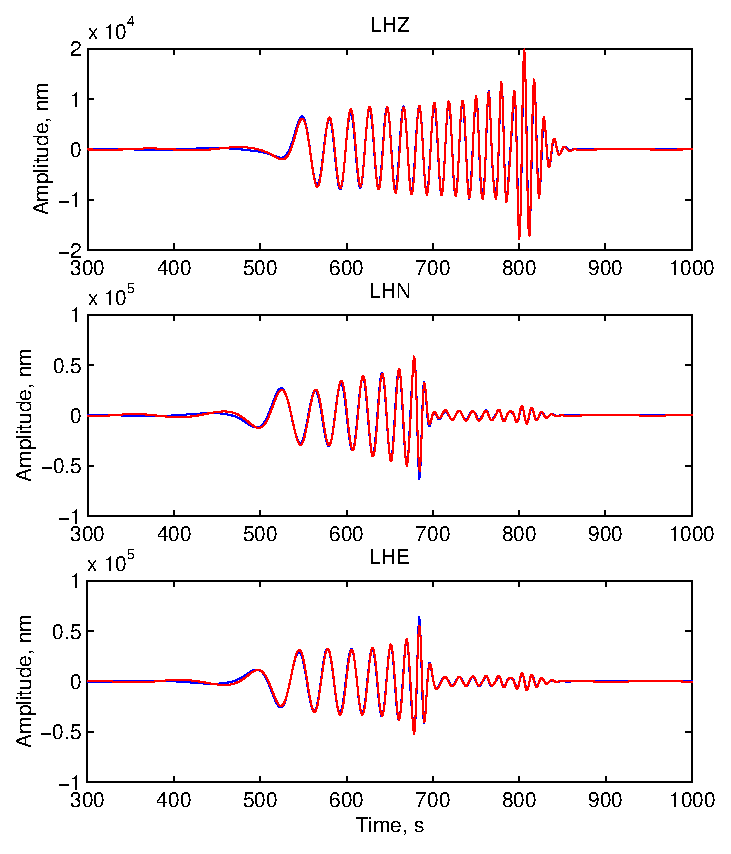
\includegraphics[width=5 in]{Figures/Fig1a}
\caption{Station BJT. Comparison with Herrmann's plane code. 
Three-component synthetic seismogram for the fundamental spheroidal and toroidal modes. 
{\bf Mineos} seismogram is plotted in red, Herrmann's in blue. Earthquake is 
25.39N, 101.40E (Southern China), depth is 33 km. Model is 
PREM, in which the water layer is filled with the upper crust's velocities.
The crust has only two layers.
}
\label{fig:1a}
\end{center}
\end{figure}
%Figure 2
\begin{figure}
\begin{center}
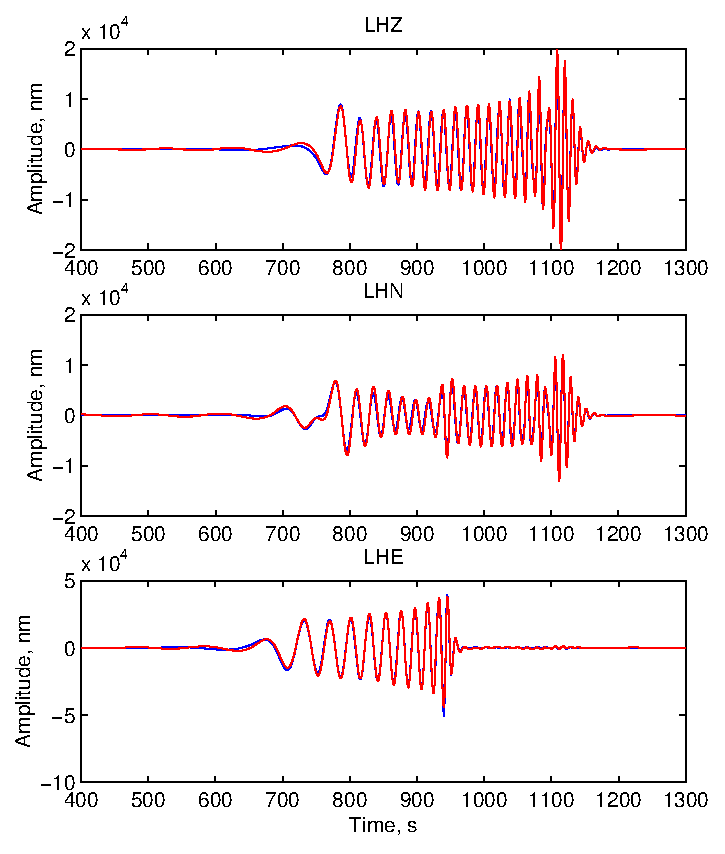
\includegraphics[width=5 in]{Figures/Fig2a}
\caption{Comparison with Herrmann's plane code, as in Figure \ref{fig:1a}, but for 
station TLY.} 
\label{fig:2a}
\end{center}
\end{figure}
%Figure 3
\begin{figure}
\begin{center}
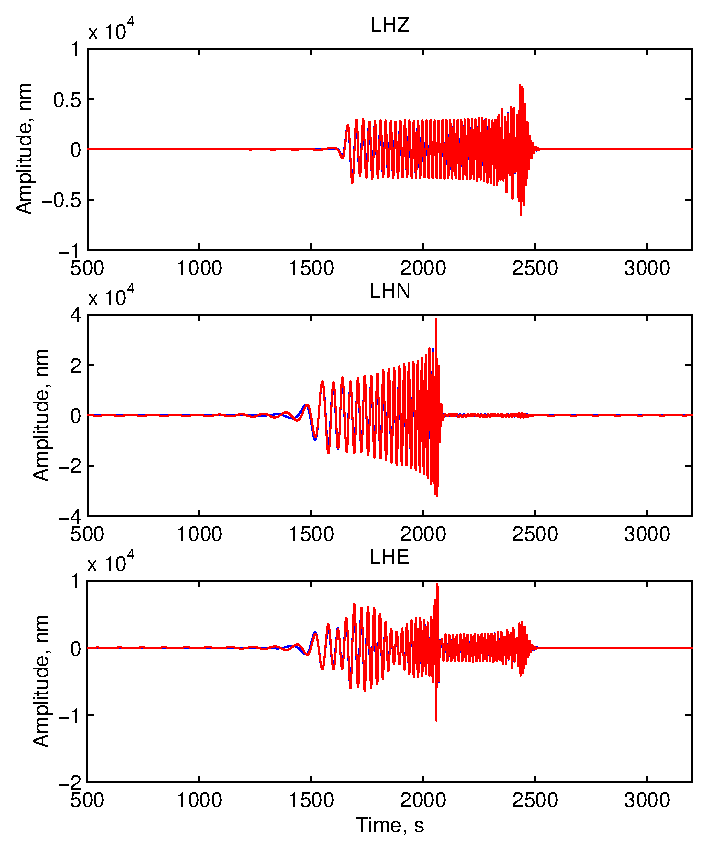
\includegraphics[width=5 in]{Figures/Fig3a}
\caption{Comparison with Herrmann's plane code, as in Figure \ref{fig:1a}, but for 
station BILL.} 
\label{fig:3a}
\end{center}
\end{figure}
%Figure 4
\begin{figure}
\begin{center}
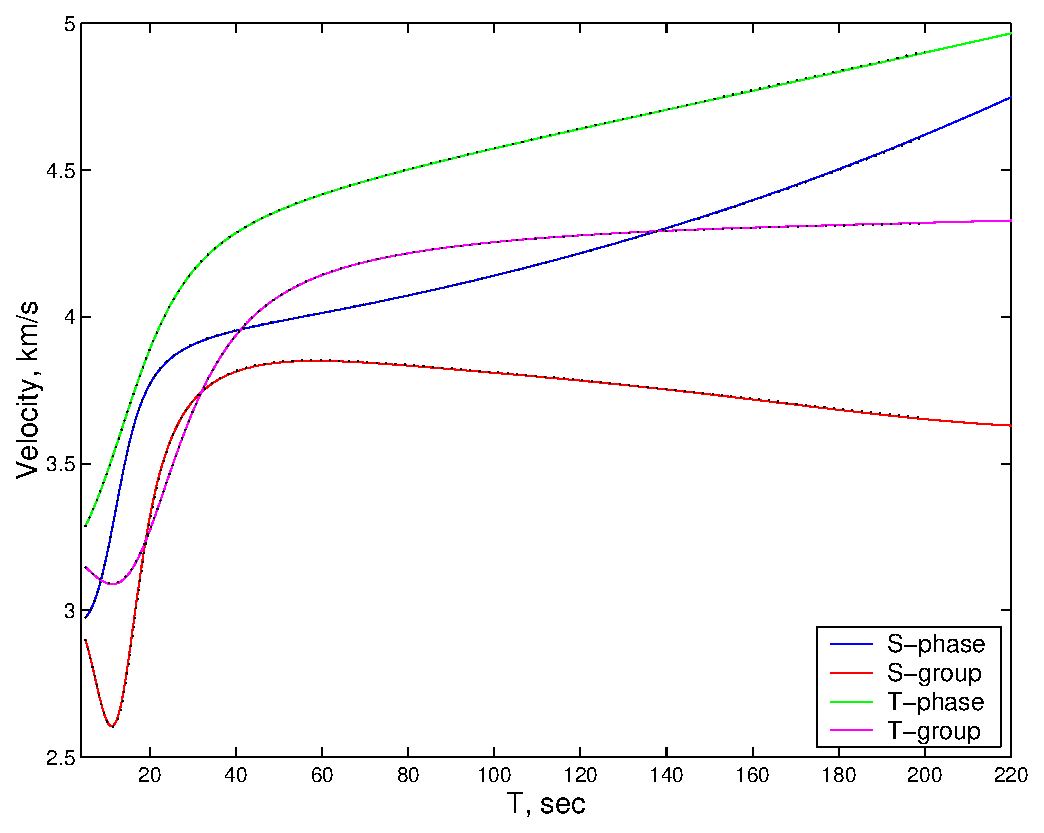
\includegraphics[width=5 in]{Figures/Fig4a}
\caption{Dispersion curves of phase and group velocities for spheroidal and totoidal
fundamental modes. The solid color lines are the {\bf Mineos} results, the 
black dotted lines are for the Herrmann's plane code. The solid lines 
color are: blue for Rayleigh phase velocity, red for Rayleigh group 
velocity, green for Love phase velocity, and magneta for group Love velocity. }
\label{fig:4a}
\end{center}
\end{figure}
% MINEOS VS SPECFM
%
\newpage
\subsection{Benchmark test \#3. Mineos vs SPECFEM3D\_GLOBE}

The  {\bf Mineos} synthetic seismograms were tested against SPECFEM3D\_GLOBE
synthetic seismograms for the same event and station set as described in 
the previous section.

\noindent \textbf{\emph{Input 1D model.}} The input model is an anisotropic, 
single-layered crust
PREM with attenuation. The 3 km water layer is filled with crustal properties.
SPECFEM3D\_GLOBE has a special subroutine for evaluation of the model parameters by 
polynomial interpolation across a fixed number of layers from the center of
the Earth up to the free surface at radius 6371 km. This polynomial 
representation was converted by a special program to a plain input file in
{\bf Mineos} format. The total number of vertical nodes is 237. The tabulated
step by depth in the crust and upper mantle is close to 1 km.

\noindent \textbf{\emph{SPECFEM3D\_GLOBE run notes.}} SPECFEM3D\_GLOBE  was configured to make
the synthetic seismogram (displacement, nm) 1 hour long. The Earth was split
into 6 chunks. Each chunk consisted of ~480x480 elements.
So, the average lateral size of the elements near to the surface was ~20x20 km.
The state of some important run parameters were: ELLIPTICITY - off,
TOPOGRAPHY - off, ROTATION - off, and GRAVITY - on. As with {\bf Mineos}, input
coordinates are geographic and geocentric coordinates are used internally.

\noindent \textbf{\emph{Mineos run notes.}} {\bf Mineos} was configured to compute all normal modes
in the frequency range $0 - 0.2$ Hz and the radial mode range $0 \le n \le 400$. 
In total, the program computed 247565 spheroidal normal modes, 162154 toroidal modes, and 
240 radial modes. Synthetic seismograms (acceleration, nm/s$^2$) 1 hour long 
were simulated. All seismograms were converted from acceleration to 
displacement in nm.

\noindent \textbf{\emph{Tapering, results discussion.}} To reduce noise at 
spectral edges, all seismograms  were half cosine tapered with corner 
frequencies $(1/200,\; 1/100)$ Hz and $(1/12, \;1/10)$ Hz.
Figures \ref{fig:5a} - \ref{fig:16a} illustrate three-component seismograms and amplitude spectra
for the BJT, TLY, and BILL stations. SPECFEM3D\_GLOBE results are plotted 
in red, {\bf Mineos} in blue.

\noindent The test shows that synthetic seismograms and spectra 
for both methods are close. Attempts to increase the high cut
frequency, say to 5 sec, lead to differences in some places with periods 
close to 8 sec. This probably resulted because the SPECFEM3D\_GLOBE spectral 
elements were not small enough.

% Station BJT

%Figure 5
\begin{figure}
\begin{center}
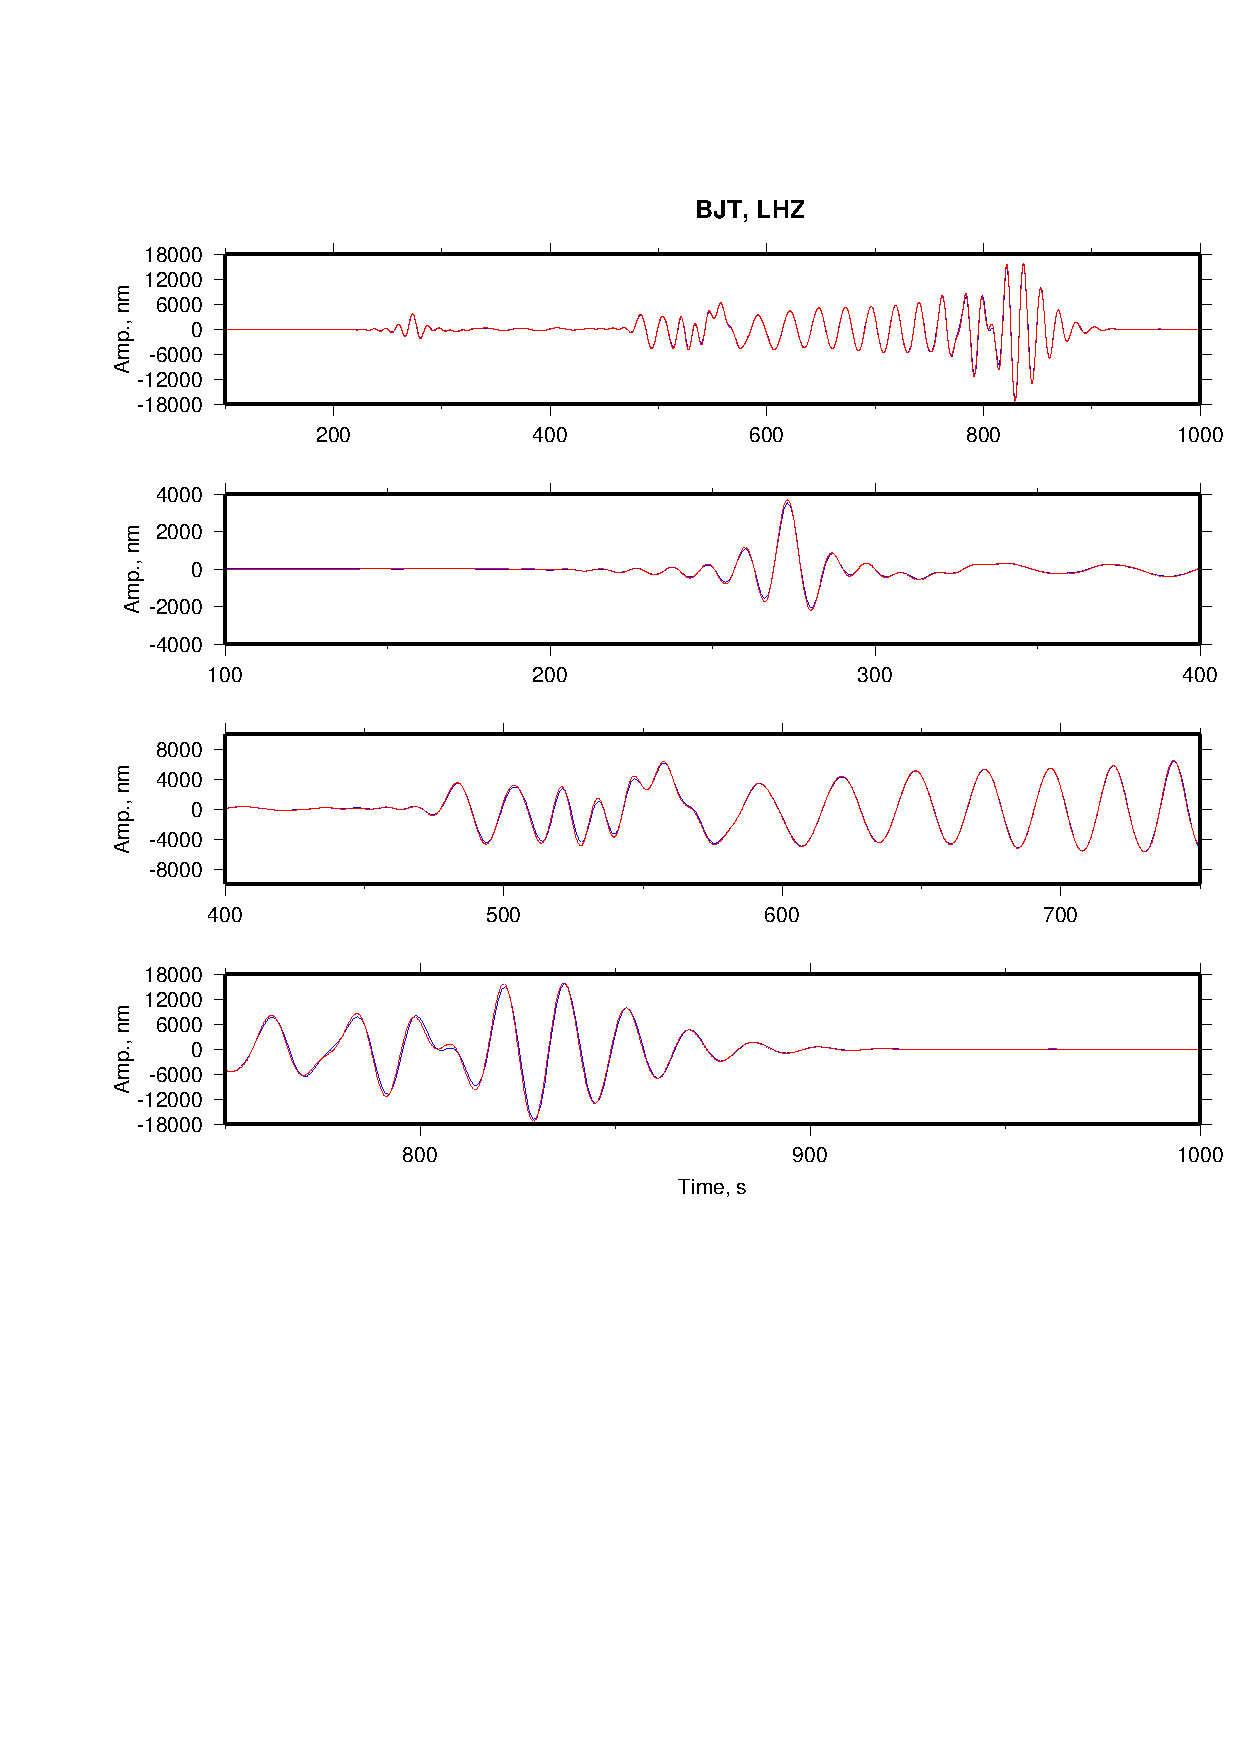
\includegraphics[width=7 in]{Figures/FigsBJTLHZ}
\caption{Synthetic seismograms for SPECFEM3D\_GLOBE (red) and {\bf Mineos} (blue). Station BJT, chan LHZ. 
Distance = $19.123^o$, Az = $-135.267^o$.
The top plot shows the whole record, the others plot separate fragments. }
\label{fig:5a}
\end{center}
\end{figure}

%Figure 6
\begin{figure}
\begin{center}
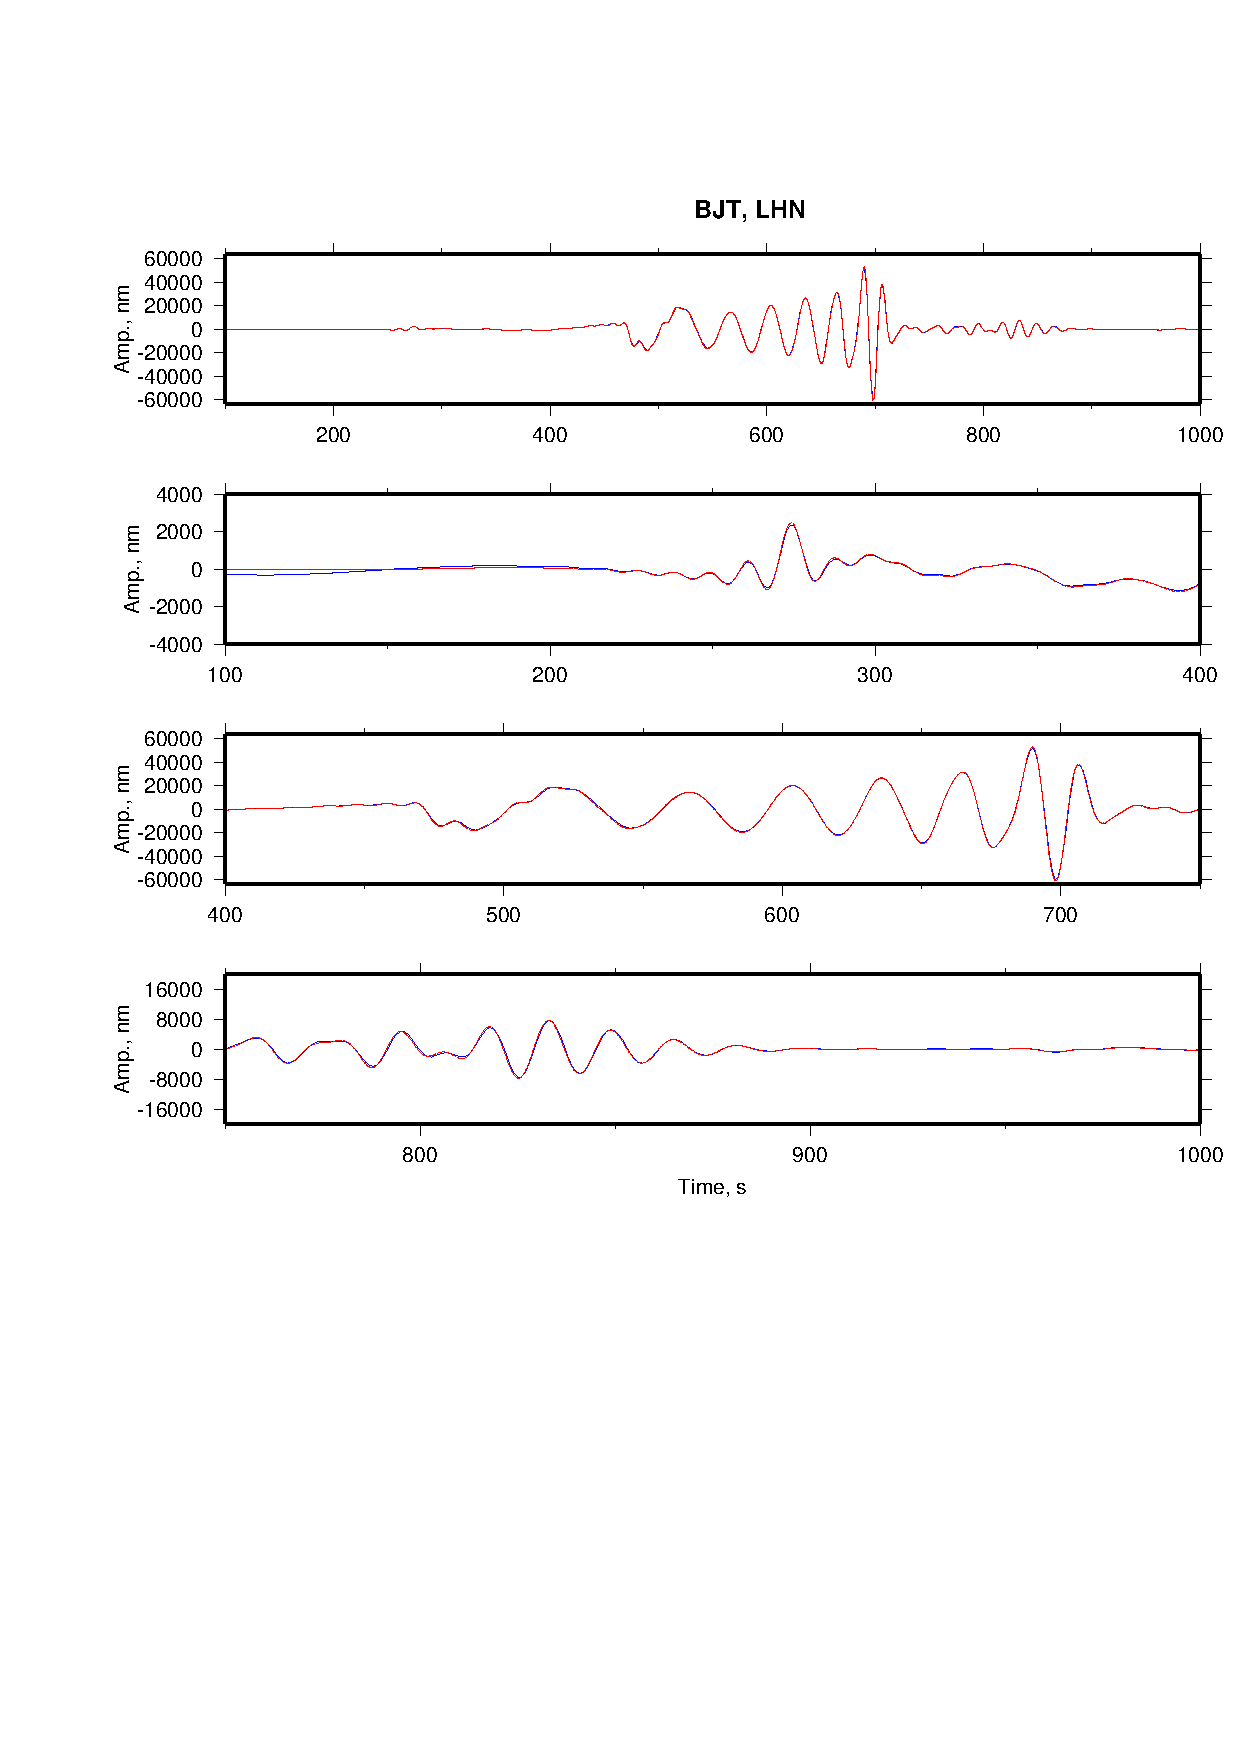
\includegraphics[width=7 in]{Figures/FigsBJTLHN}
\caption{ The same as Figure \ref{fig:5a}, but for LHN channel.}
\label{fig:6a}
\end{center}
\end{figure}

%Figure 7
\begin{figure}
\begin{center}
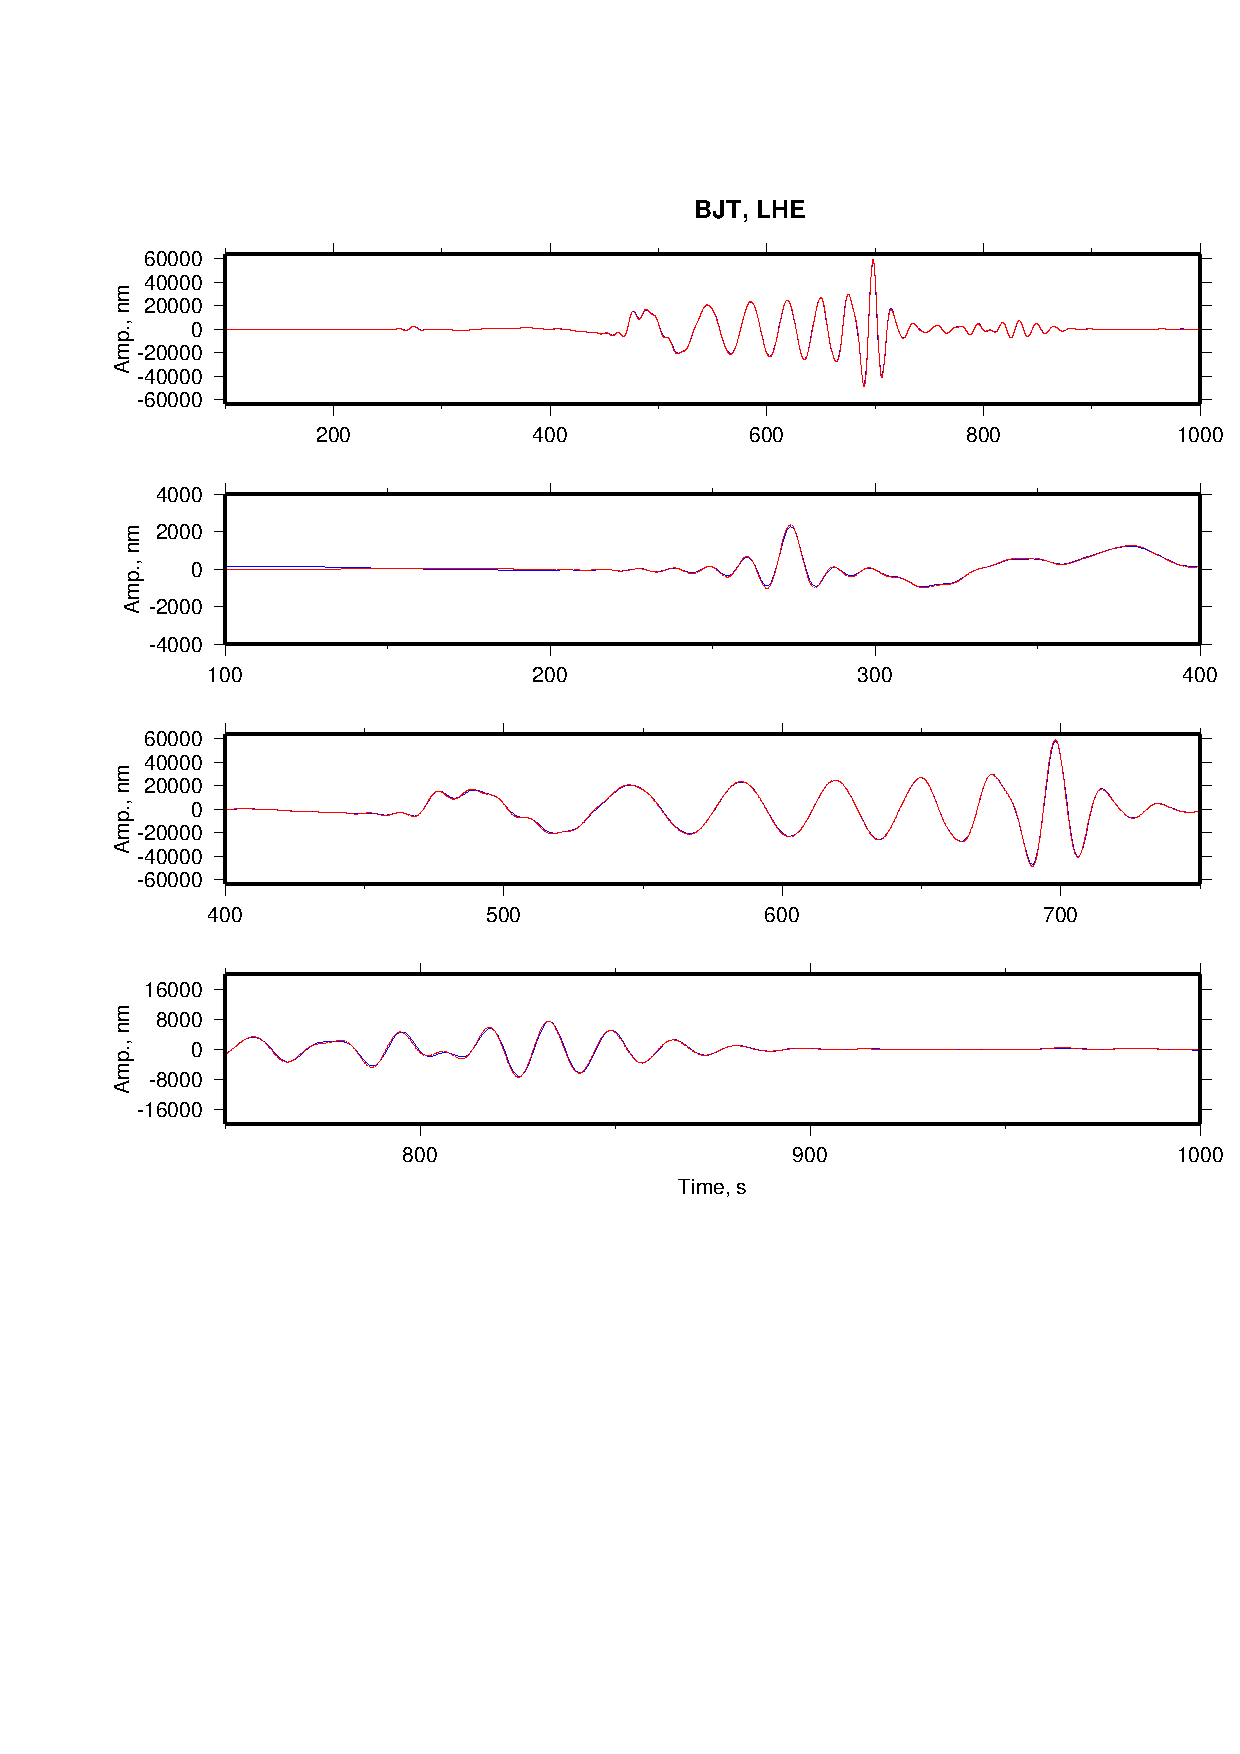
\includegraphics[width=7 in]{Figures/FigsBJTLHE}
\caption{The same as Figure \ref{fig:5a}, but for LHE channel.}
\label{fig:7a}
\end{center}
\end{figure}

%Figure 8
\begin{figure}
\begin{center}
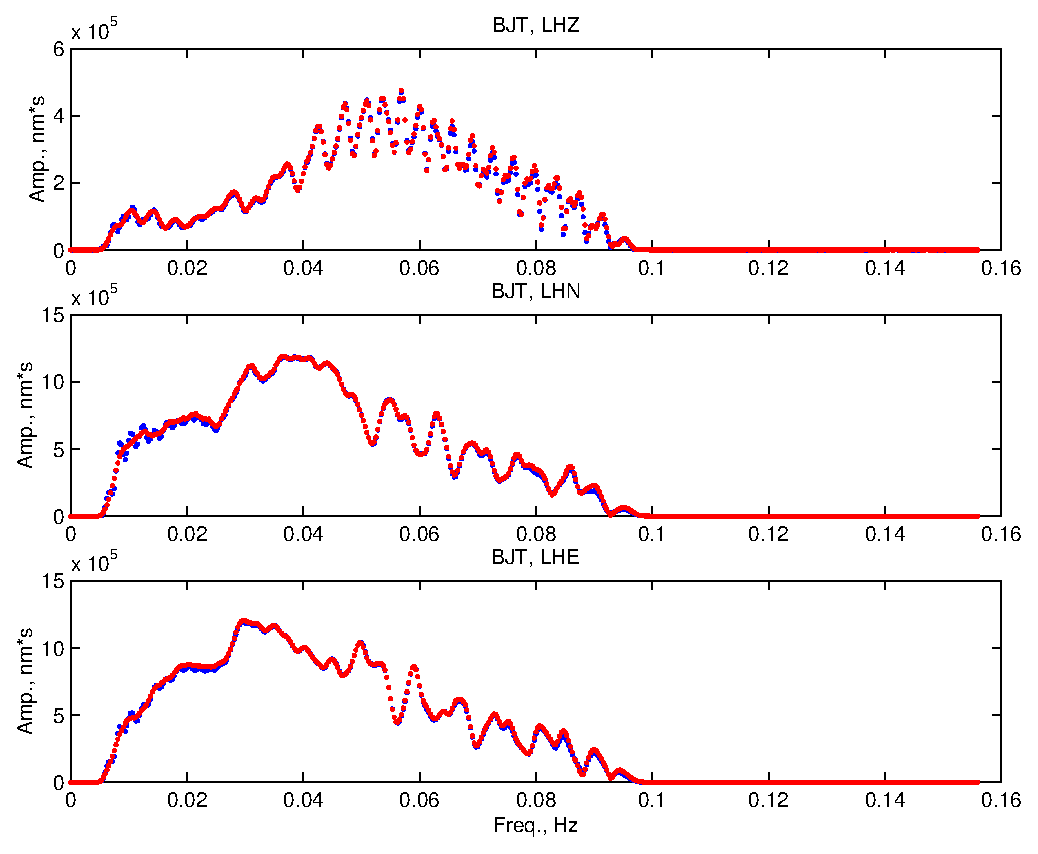
\includegraphics[width=7 in]{Figures/FspBJT}
\caption{Amplitude spectra for the station BJT. Red color - SPECFEM3D\_GLOBE spectra, blue - {\bf Mineos}.}
\label{fig:8a}
\end{center}
\end{figure}

% Station TLY 

%Figure 9
\begin{figure}
\begin{center}
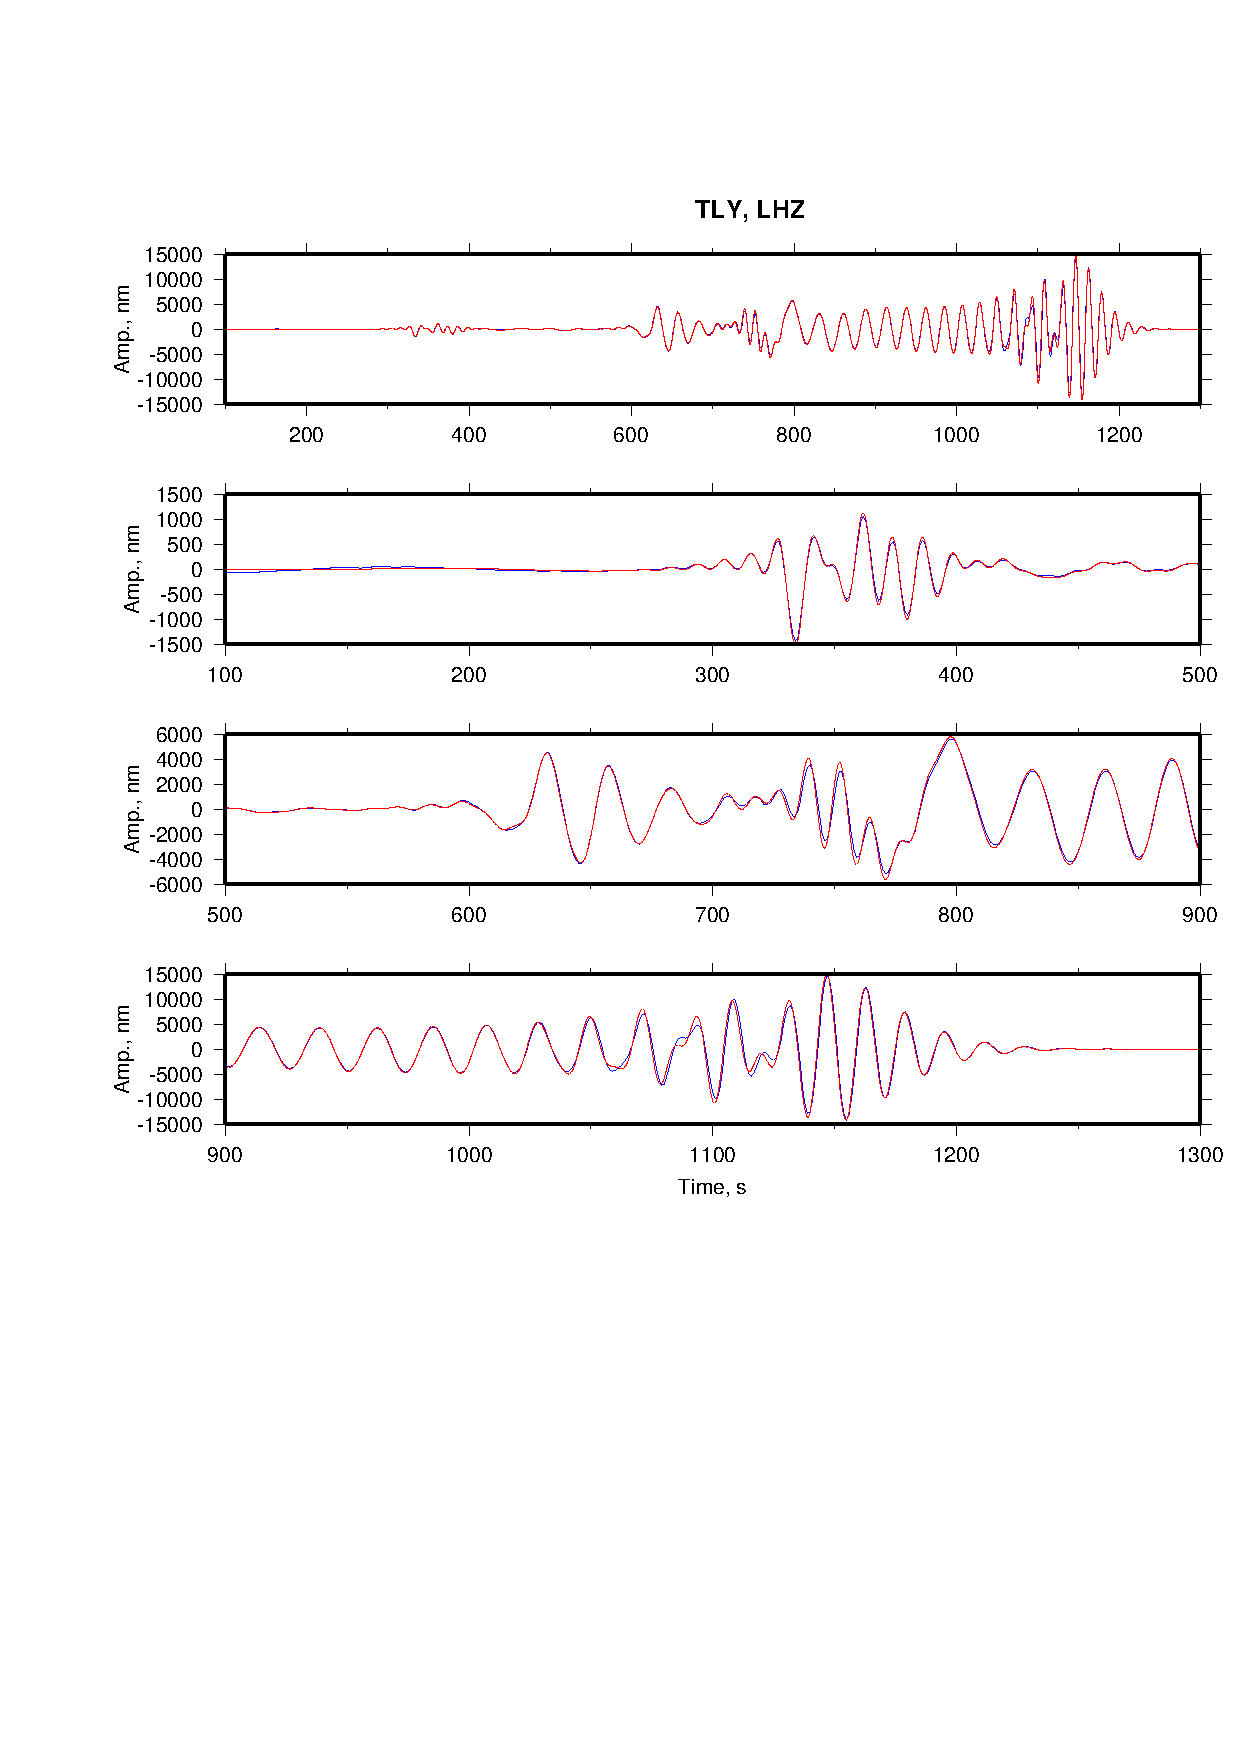
\includegraphics[width=7 in]{Figures/FigsTLYLHZ}
\caption{Synthetic seismograms for SPECFEM3D\_GLOBE (red) and {\bf Mineos} (blue). Station TLY, chan LHZ. 
Distance = $26.308^o$, Az = $-175,417^o$.
The top plot shows the whole record, the others plot separate fragments. }
\label{fig:9a}
\end{center}
\end{figure}

%Figure 10
\begin{figure}
\begin{center}
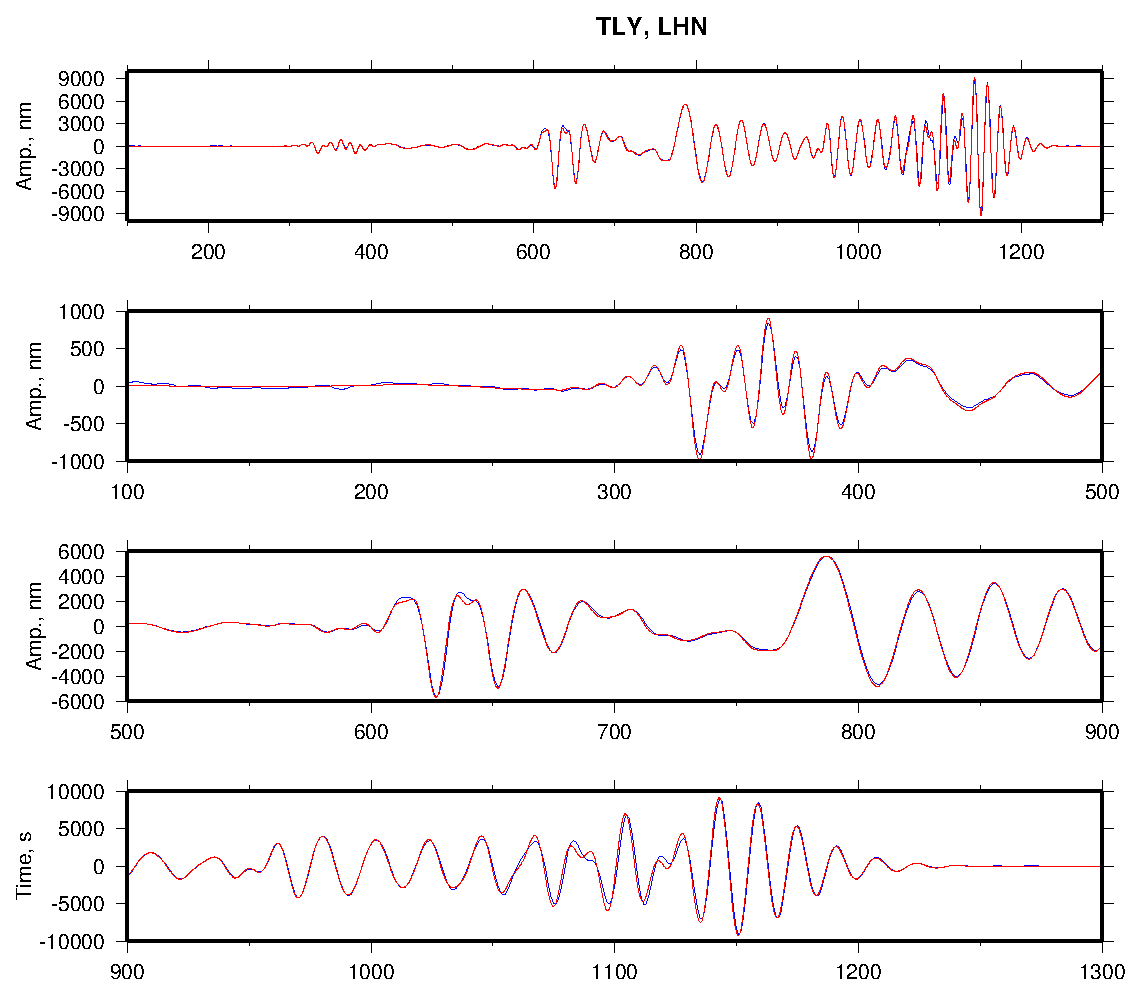
\includegraphics[width=7 in]{Figures/FigsTLYLHN}
\caption{ The same as Figure \ref{fig:9a}, but for LHN channel.}
\label{fig:10a}
\end{center}
\end{figure}

%Figure 11
\begin{figure}
\begin{center}
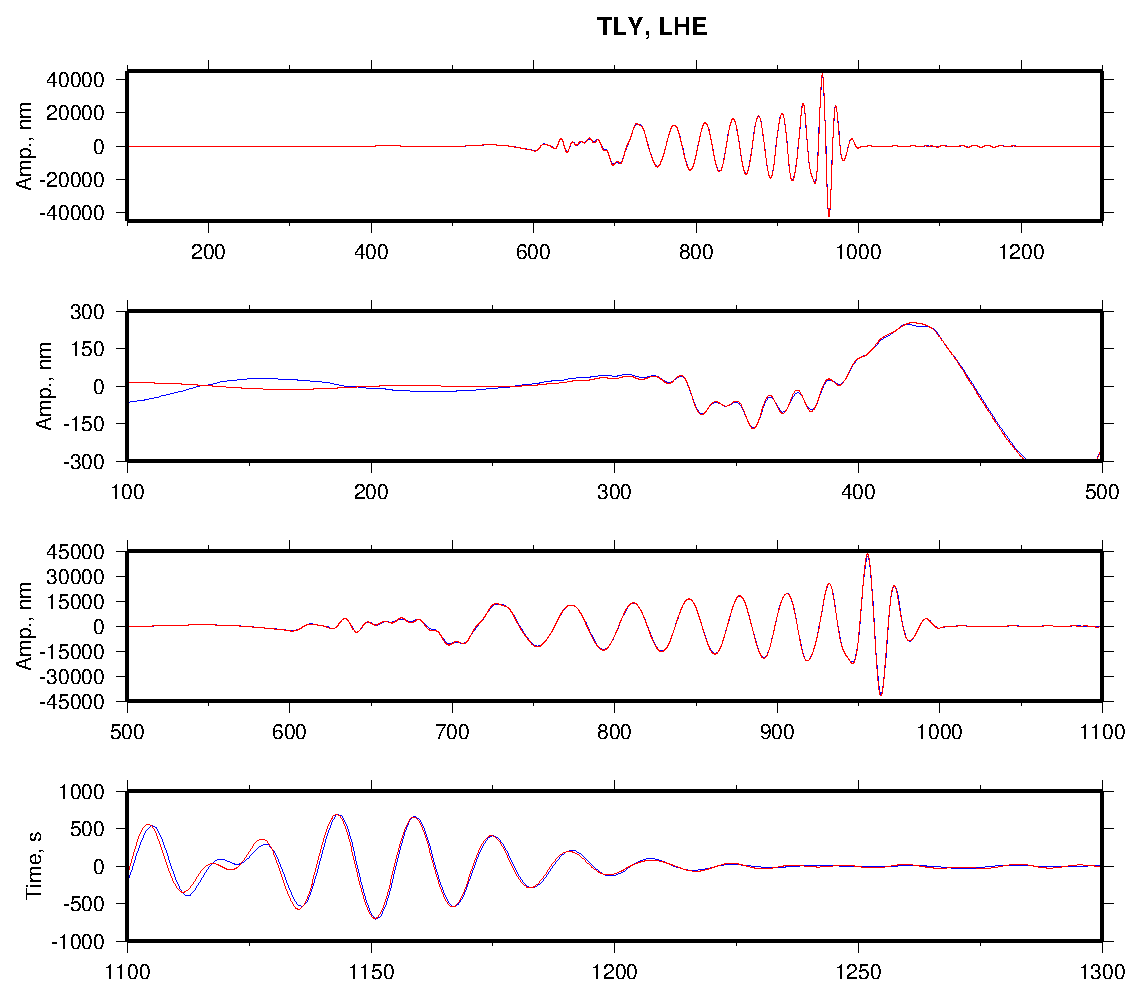
\includegraphics[width=7 in]{Figures/FigsTLYLHE}
\caption{ The same as Figure \ref{fig:9a}, but for LHE channel.}
\label{fig:11a}
\end{center}
\end{figure}

%Figure 12
\begin{figure}
\begin{center}
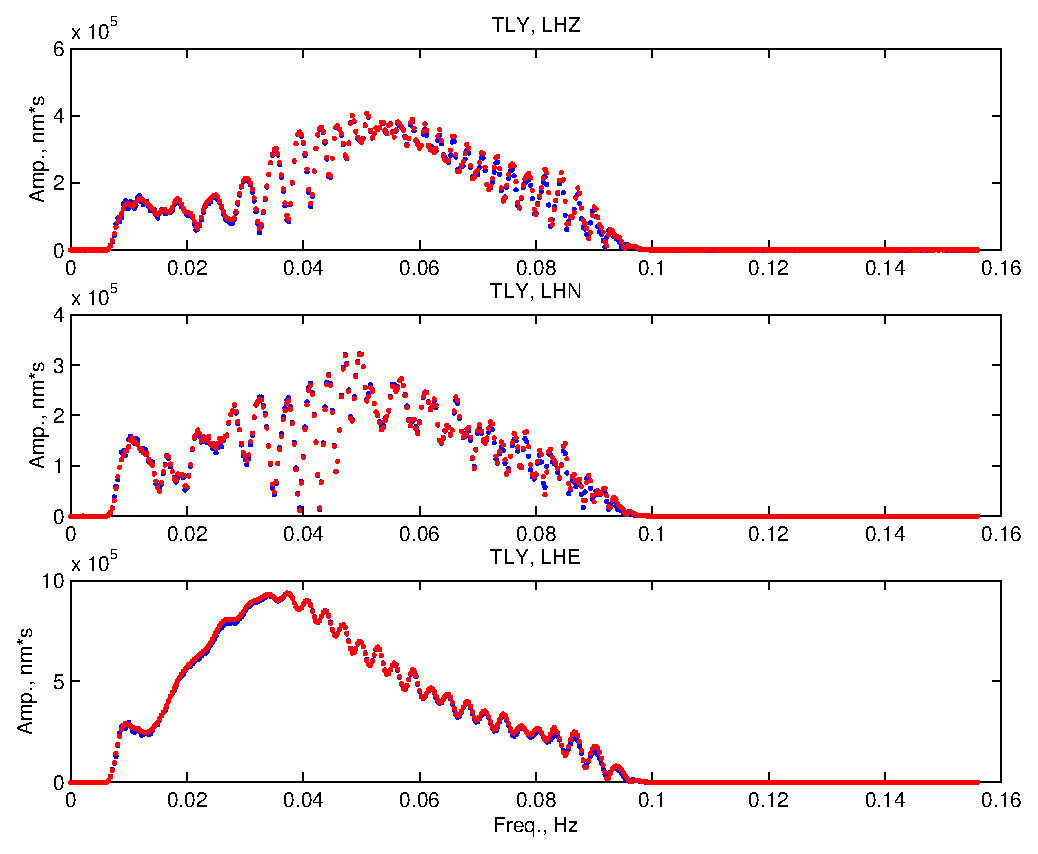
\includegraphics[width=7 in]{Figures/FspTLY}
\caption{Amplitude spectra for the station TLY. Red color - SPECFEM3D\_GLOBE spectra, blue - {\bf Mineos}.}
\label{fig:12a}
\end{center}
\end{figure}

% Station BILL

%Figure 13
\begin{figure}
\begin{center}
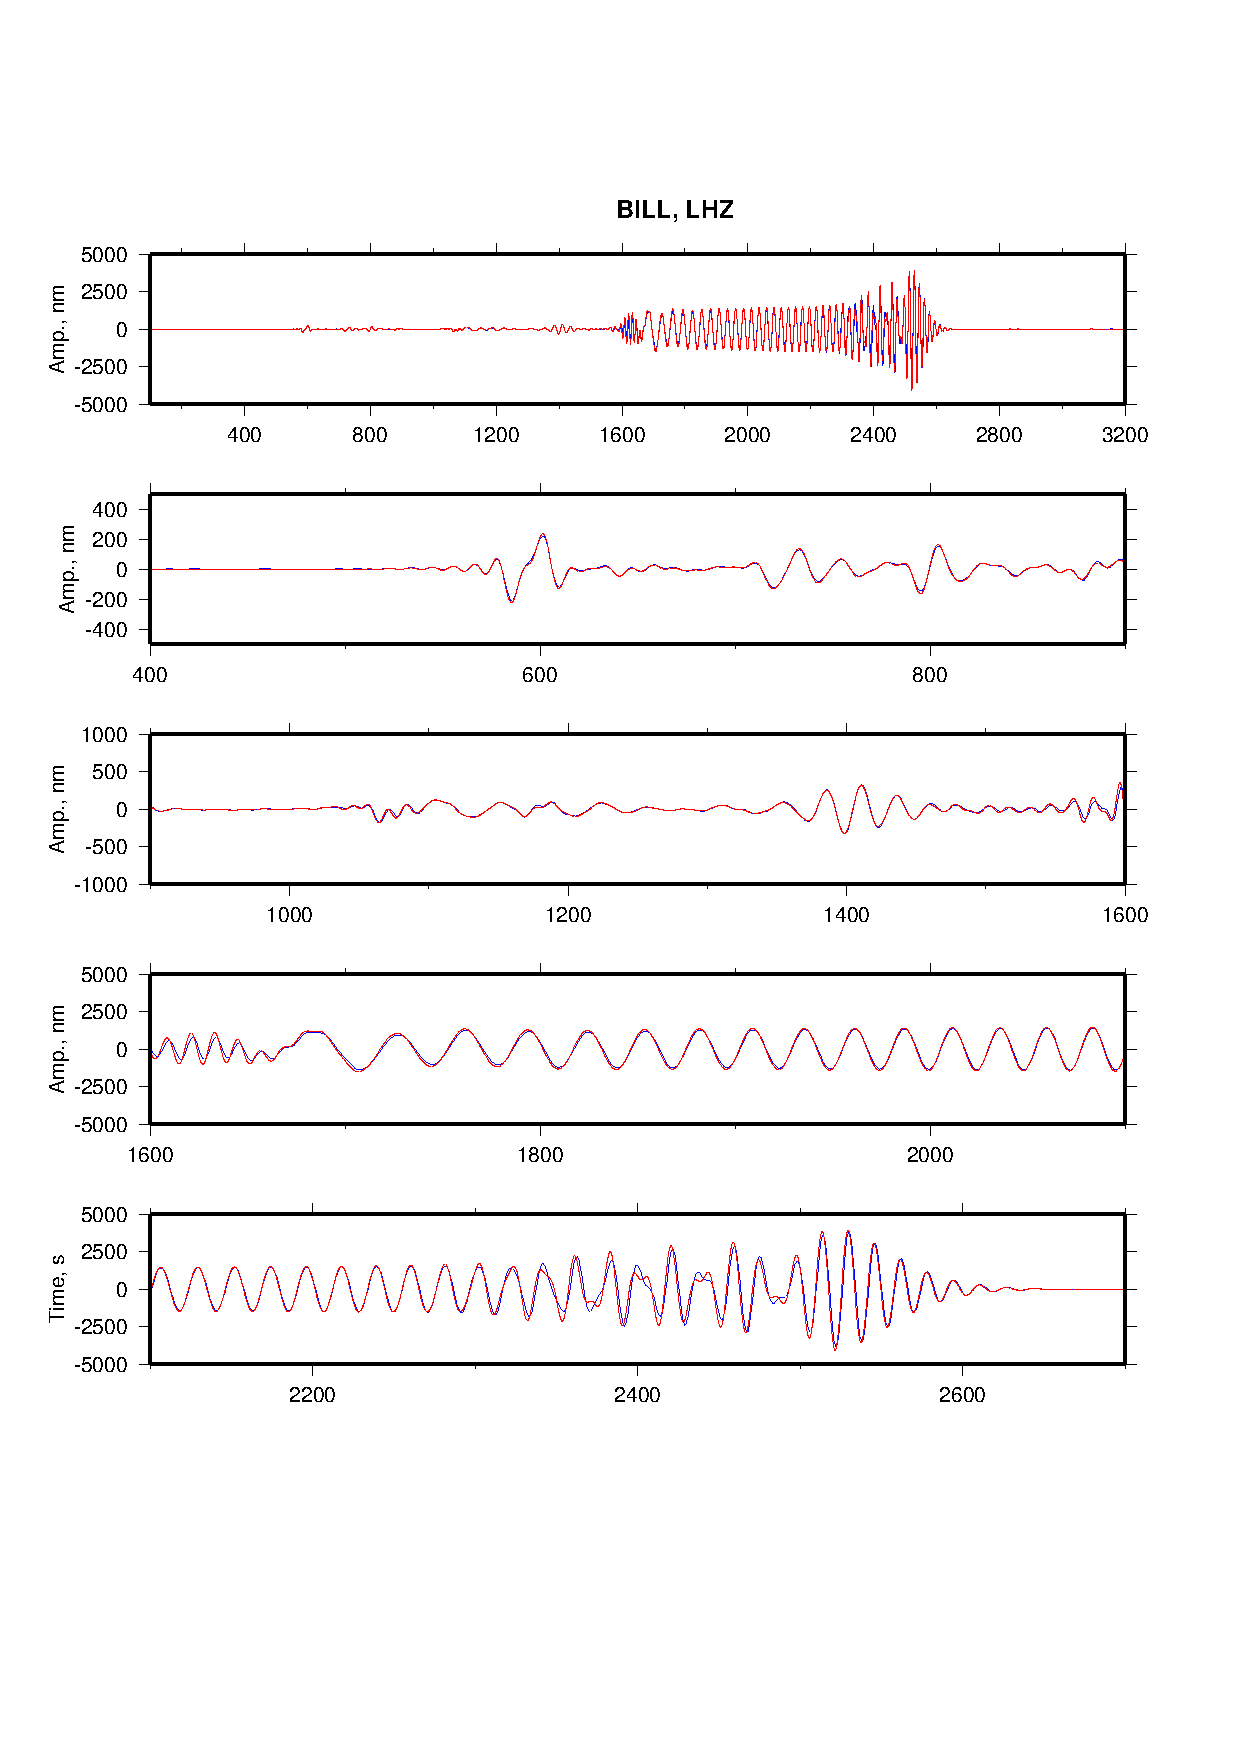
\includegraphics[width=7 in]{Figures/FigsBILLLHZ}
\caption{Synthetic seismograms for SPECFEM3D\_GLOBE (red) and {\bf Mineos} (blue). Station BILL, chan LHZ. 
Distance = $57.417^o$, Az = $-103.266^o$.
The top plot shows the whole record, the others plot separate fragments. }
\label{fig:13a}
\end{center}
\end{figure}

%Figure 14
\begin{figure}
\begin{center}
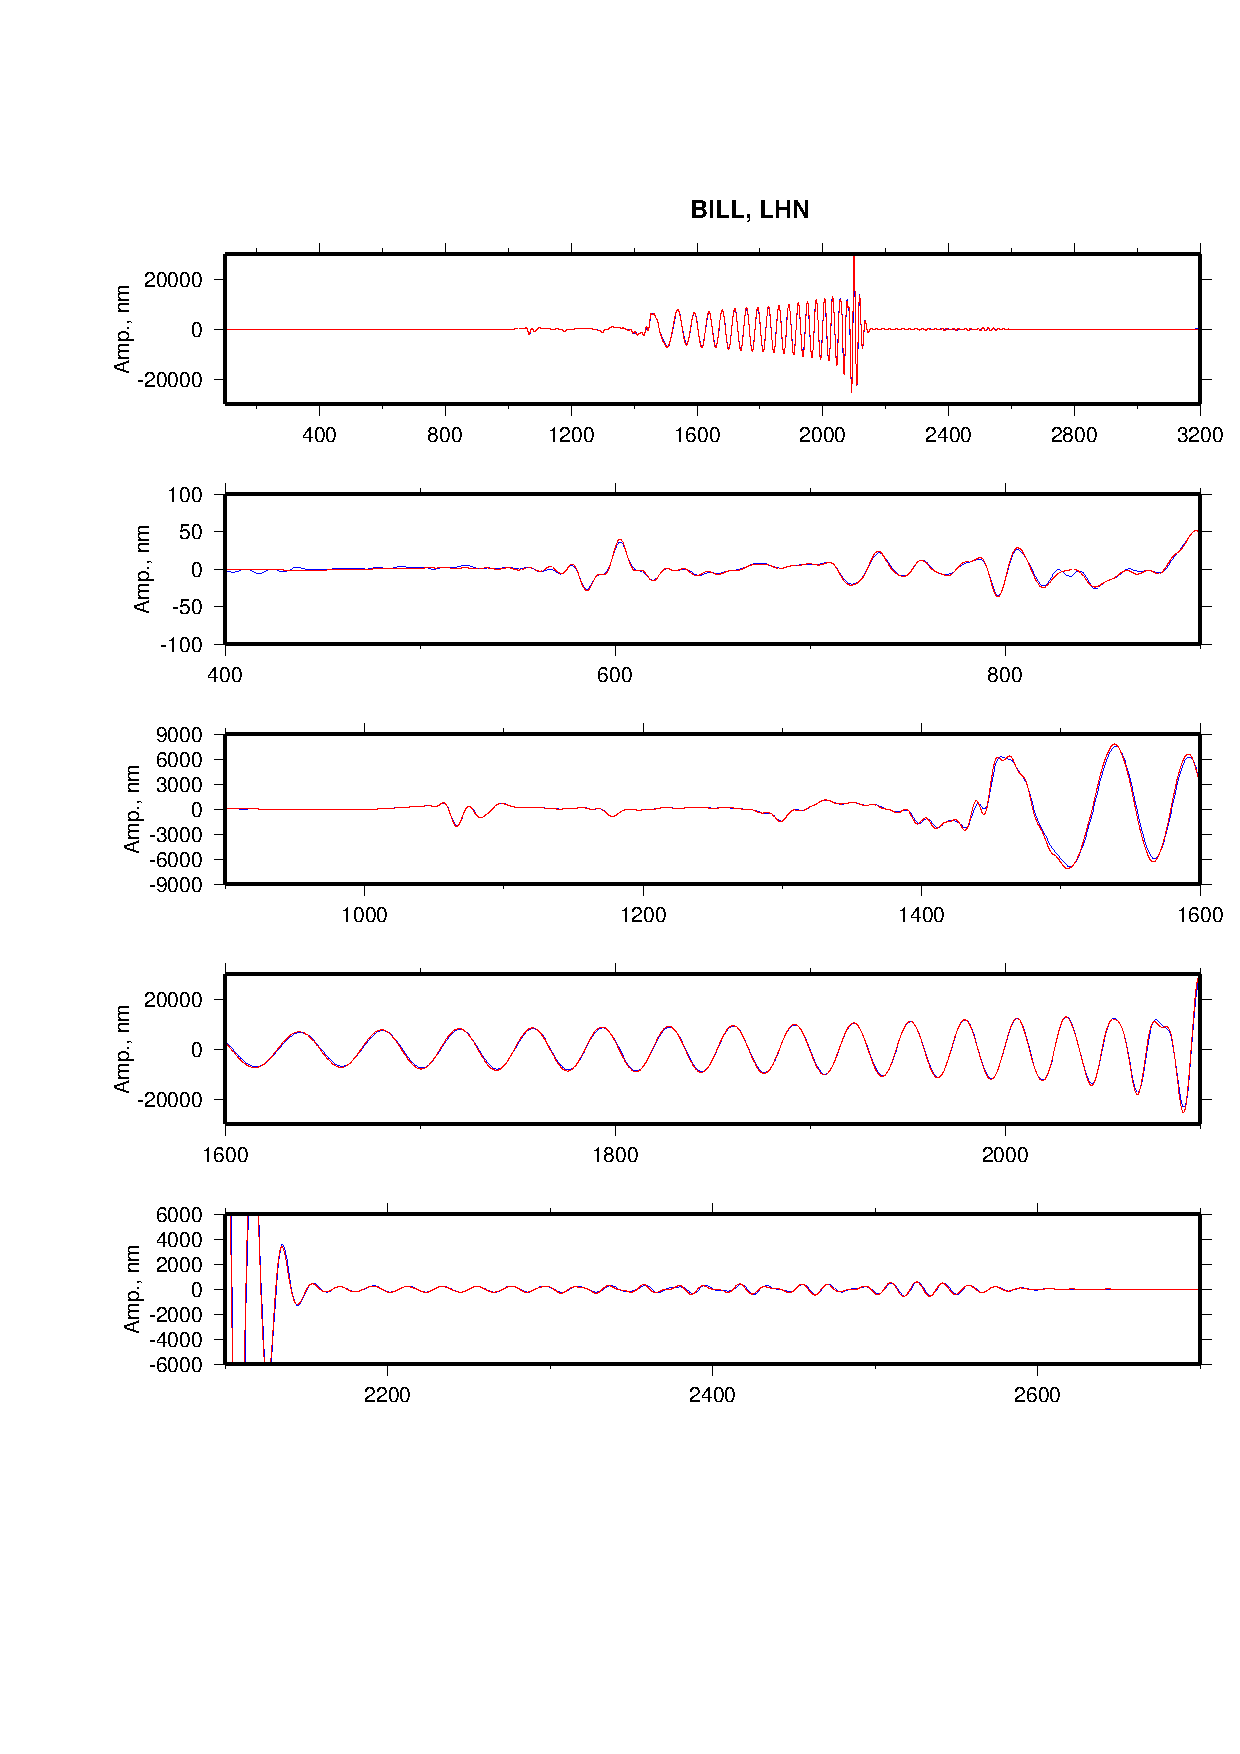
\includegraphics[width=7 in]{Figures/FigsBILLLHN}
\caption{ The same as Figure \ref{fig:13a}, but for LHN channel.}
\label{fig:14a}
\end{center}
\end{figure}

%Figure 15
\begin{figure}
\begin{center}
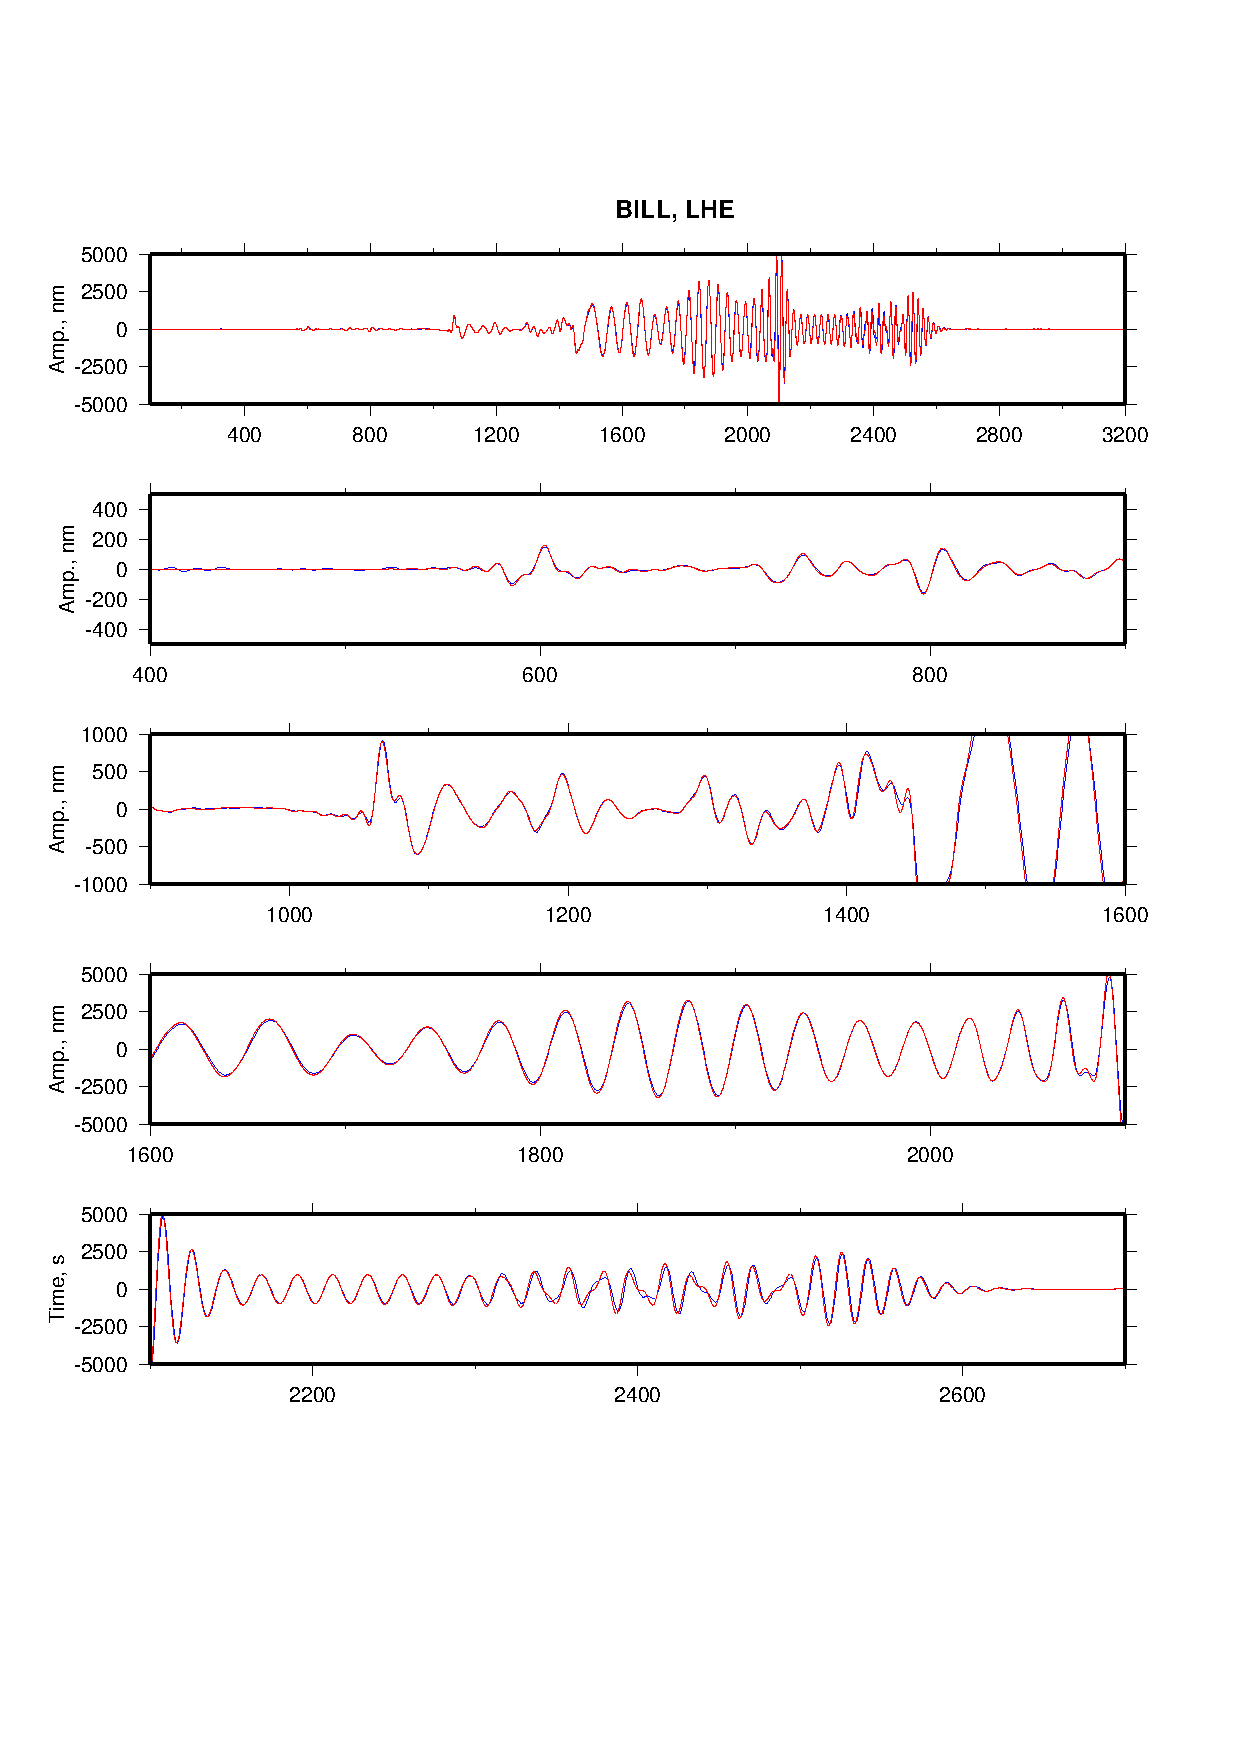
\includegraphics[width=7 in]{Figures/FigsBILLLHE}
\caption{ The same as Figure \ref{fig:13a}, but for LHE channel.}
\label{fig:15a}
\end{center}
\end{figure}

%Figure 16
\begin{figure}
\begin{center}
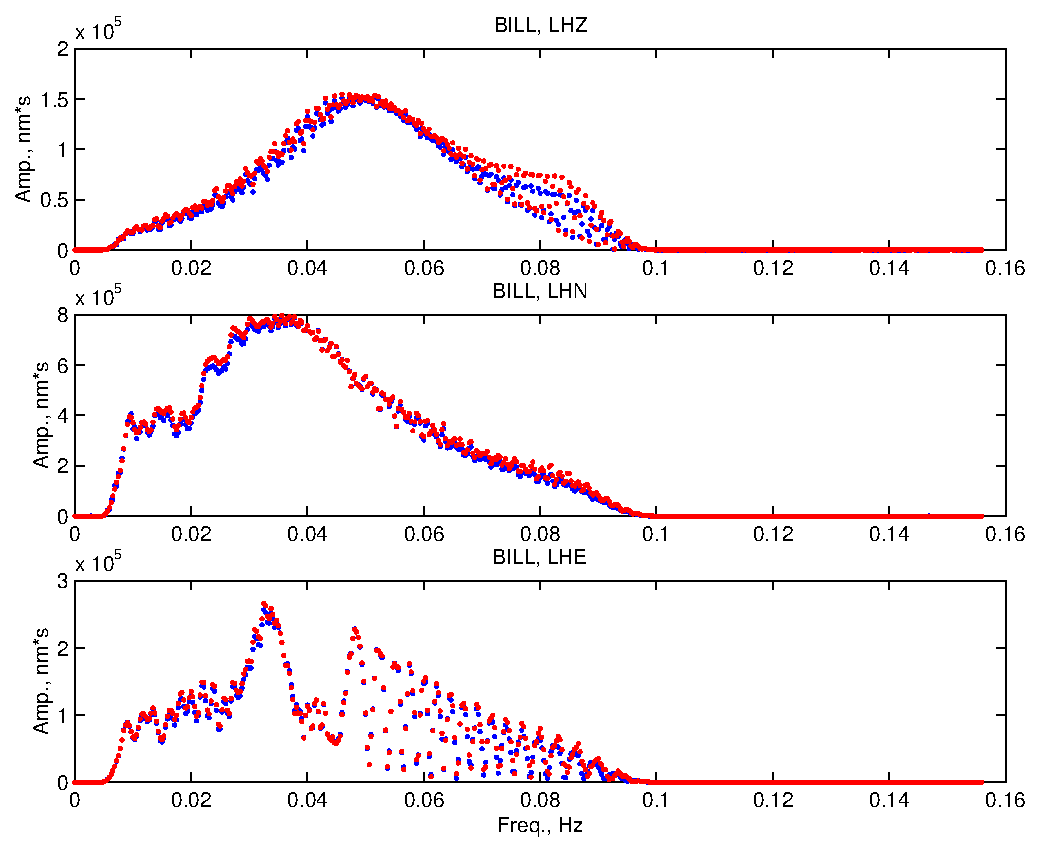
\includegraphics[width=7 in]{Figures/FspBILL}
\caption{Amplitude spectra for the station BILL. Red color - SPECFEM3D\_GLOBE spectra, blue - {\bf Mineos}.}
\label{fig:16a}
\end{center}
\end{figure}


\section {Reference Frame Convention}
The {\bf Mineos} code uses the following convention for the Cartesian reference frame defining the standard sensor orientation:
\begin{itemize}
\item the $x$ axis points East
\item the $y$ axis points North
\item the $z$ axis points up
\end{itemize}
Note that this convention is the same as for {\bf SPECFEM3D\_GLOBE} code, and it is
different from the Harvard Centroid-Moment Tensor 
(CMT) convention. The Harvard CMT convention is
\begin{itemize}
\item the $x$ axis points South
\item the $y$ axis points East
\item the $z$ axis points up
\end{itemize}

\end{document}
